% =====================================================================
% Nanograph -- Nature Methods-style manuscript.
% All run-dependent numbers come from numbers.tex and tables/*.tex, which
% paper/make_numbers.py regenerates from the evaluation outputs.
% =====================================================================
\documentclass[10pt,a4paper]{article}

\usepackage[T1]{fontenc}
\usepackage{lmodern}
\usepackage[margin=2.5cm]{geometry}
\usepackage{graphicx}
\usepackage{booktabs}
\usepackage{amsmath}
\usepackage{amssymb}
\usepackage{xcolor}
\usepackage{xspace}
\usepackage{microtype}
\usepackage[numbers,sort&compress]{natbib}
\usepackage{authblk}
\usepackage{lineno}
\usepackage{titlesec}
\usepackage{adjustbox}
\usepackage[font=small,labelfont=bf]{caption}
\usepackage[hidelinks]{hyperref}

\newcommand{\method}{\textnormal{\textsc{Nanograph}}\xspace}
\providecommand{\tbd}{\textcolor{red}{[TBD]}}
% AUTO-GENERATED by paper/make_numbers.py -- do not edit by hand.
\providecommand{\tbd}{\textcolor{red}{[TBD]}}
\newcommand{\RunCommit}{39a8c5d}
\newcommand{\DBytes}{2200\pm319}
\newcommand{\DBytesm}{2200}
\newcommand{\DNodes}{158\pm36}
\newcommand{\DNodesm}{158}
\newcommand{\DEdges}{158\pm37}
\newcommand{\DEdgesm}{158}
\newcommand{\DTime}{1154\pm209}
\newcommand{\DTimem}{1154}
\newcommand{\DFGPSNR}{28.09\pm0.56}
\newcommand{\DFGPSNRm}{28.09}
\newcommand{\DFGSSIM}{0.9992\pm0.0003}
\newcommand{\DFGSSIMm}{0.9992}
\newcommand{\DGTFGPSNR}{27.30\pm2.04}
\newcommand{\DGTFGPSNRm}{27.30}
\newcommand{\DGTFGSSIM}{0.9988\pm0.0015}
\newcommand{\DGTFGSSIMm}{0.9988}
\newcommand{\DFullPSNR}{30.76\pm0.62}
\newcommand{\DFullPSNRm}{30.76}
\newcommand{\DFullSSIM}{0.562\pm0.027}
\newcommand{\DFullSSIMm}{0.562}
\newcommand{\DSegIoU}{0.870\pm0.106}
\newcommand{\DSegIoUm}{0.870}
\newcommand{\DSegPrec}{0.932\pm0.027}
\newcommand{\DSegPrecm}{0.932}
\newcommand{\DSegRec}{0.928\pm0.112}
\newcommand{\DSegRecm}{0.928}
\newcommand{\DGTIoU}{0.646\pm0.104}
\newcommand{\DGTIoUm}{0.646}
\newcommand{\DBetaZero}{4.41\pm0.73}
\newcommand{\DBetaZerom}{4.41}
\newcommand{\DBetaOne}{0.32\pm0.61}
\newcommand{\DBetaOnem}{0.32}
\newcommand{\DCycles}{3.66\pm3.16}
\newcommand{\DCyclesm}{3.66}
\newcommand{\DWidth}{2.98\pm0.44}
\newcommand{\DWidthm}{2.98}
\newcommand{\DVsRaw}{30.6\pm6.1}
\newcommand{\DVsRawm}{30.6}
\newcommand{\DVsPNG}{21.2\pm4.2}
\newcommand{\DVsPNGm}{21.2}
\newcommand{\DJpegBytes}{2150\pm291}
\newcommand{\DJpegBytesm}{2150}
\newcommand{\DJpegFullPSNR}{31.16\pm0.51}
\newcommand{\DJpegFullPSNRm}{31.16}
\newcommand{\DJpegFullSSIM}{0.609\pm0.026}
\newcommand{\DJpegFullSSIMm}{0.609}
\newcommand{\DJpegFGPSNR}{27.90\pm0.74}
\newcommand{\DJpegFGPSNRm}{27.90}
\newcommand{\DJpegGTFGPSNR}{27.90\pm0.72}
\newcommand{\DJpegGTFGPSNRm}{27.90}
\newcommand{\DJpegGTIoU}{0.652\pm0.082}
\newcommand{\DJpegGTIoUm}{0.652}
\newcommand{\DJpegBetti}{0.105\pm0.232}
\newcommand{\DJpegBettim}{0.105}
\newcommand{\DJpegBetaZero}{9.29\pm3.65}
\newcommand{\DJpegBetaZerom}{9.29}
\newcommand{\DJpegBetaOne}{3.97\pm3.66}
\newcommand{\DJpegBetaOnem}{3.97}
\newcommand{\DWebpBytes}{2096\pm322}
\newcommand{\DWebpBytesm}{2096}
\newcommand{\DWebpFullPSNR}{31.43\pm0.49}
\newcommand{\DWebpFullPSNRm}{31.43}
\newcommand{\DWebpFullSSIM}{0.650\pm0.026}
\newcommand{\DWebpFullSSIMm}{0.650}
\newcommand{\DWebpFGPSNR}{27.58\pm0.67}
\newcommand{\DWebpFGPSNRm}{27.58}
\newcommand{\DJtwoBytes}{4177\pm565}
\newcommand{\DJtwoBytesm}{4177}
\newcommand{\DJtwoFullPSNR}{31.91\pm0.50}
\newcommand{\DJtwoFullPSNRm}{31.91}
\newcommand{\DJtwoFullSSIM}{0.700\pm0.026}
\newcommand{\DJtwoFullSSIMm}{0.700}
\newcommand{\DJtwoFGPSNR}{30.90\pm0.76}
\newcommand{\DJtwoFGPSNRm}{30.90}
\newcommand{\DSelfIoU}{0.675\pm0.104}
\newcommand{\DSelfIoUm}{0.675}
\newcommand{\DN}{726}
\newcommand{\DGTIoUWins}{385/715}
\newcommand{\DGTIoUWinsPct}{53.8}
\newcommand{\DGTIoUWinsP}{0.04}
\newcommand{\DGTIoUWinsCI}{[-0.0043,+0.0026]}
\newcommand{\DGTFGPSNRWins}{154/715}
\newcommand{\DGTFGPSNRWinsPct}{21.5}
\newcommand{\DGTFGPSNRWinsP}{3.5\times10^{-55}}
\newcommand{\DGTFGPSNRWinsCI}{\tbd}
\newcommand{\DFGPSNRWins}{526/715}
\newcommand{\DFGPSNRWinsPct}{73.6}
\newcommand{\DFGPSNRWinsP}{1.3\times10^{-37}}
\newcommand{\DFGPSNRWinsCI}{\tbd}
\newcommand{\DSelfIoUWinsJpeg}{526/715}
\newcommand{\DSelfIoUWinsJpegPct}{73.6}
\newcommand{\DSelfIoUWinsJpegP}{1.3\times10^{-37}}
\newcommand{\DSelfIoUWinsJpegCI}{[+0.0167,+0.0239]}
\newcommand{\DSelfIoUWinsWebp}{652/726}
\newcommand{\DSelfIoUWinsWebpPct}{89.8}
\newcommand{\DSelfIoUWinsWebpP}{2.1\times10^{-116}}
\newcommand{\DSelfIoUWinsWebpCI}{\tbd}
\newcommand{\DSelfIoUWinsJtwo}{605/706}
\newcommand{\DSelfIoUWinsJtwoPct}{85.7}
\newcommand{\DSelfIoUWinsJtwoP}{2.2\times10^{-88}}
\newcommand{\DSelfIoUWinsJtwoCI}{\tbd}
\newcommand{\DHeldN}{108}
\newcommand{\DHeldSegIoU}{0.863\pm0.119}
\newcommand{\DHeldSegIoUm}{0.863}
\newcommand{\DHeldGTIoUWins}{54/105}
\newcommand{\DHeldGTIoUWinsPct}{51.4}
\newcommand{\DHeldGTIoUWinsP}{0.85}
\newcommand{\DHeldGTIoUWinsCI}{\tbd}
\newcommand{\DAPRR}{0.00242}
\newcommand{\DBRR}{0.0336}
\newcommand{\DBPP}{13.9}
\newcommand{\DFewerX}{7.6}
\newcommand{\DRicherX}{6.9}
\newcommand{\DBRRvsGU}{-8}
\newcommand{\CBytes}{2871\pm1243}
\newcommand{\CBytesm}{2871}
\newcommand{\CNodes}{157\pm82}
\newcommand{\CNodesm}{157}
\newcommand{\CEdges}{156\pm83}
\newcommand{\CEdgesm}{156}
\newcommand{\CTime}{2406\pm1302}
\newcommand{\CTimem}{2406}
\newcommand{\CFGPSNR}{29.04\pm0.71}
\newcommand{\CFGPSNRm}{29.04}
\newcommand{\CFGSSIM}{0.9955\pm0.0032}
\newcommand{\CFGSSIMm}{0.9955}
\newcommand{\CGTFGPSNR}{24.91\pm4.12}
\newcommand{\CGTFGPSNRm}{24.91}
\newcommand{\CGTFGSSIM}{0.9974\pm0.0029}
\newcommand{\CGTFGSSIMm}{0.9974}
\newcommand{\CFullPSNR}{30.06\pm1.09}
\newcommand{\CFullPSNRm}{30.06}
\newcommand{\CFullSSIM}{0.556\pm0.030}
\newcommand{\CFullSSIMm}{0.556}
\newcommand{\CSegIoU}{0.366\pm0.122}
\newcommand{\CSegIoUm}{0.366}
\newcommand{\CSegPrec}{0.437\pm0.178}
\newcommand{\CSegPrecm}{0.437}
\newcommand{\CSegRec}{0.849\pm0.226}
\newcommand{\CSegRecm}{0.849}
\newcommand{\CGTIoU}{0.564\pm0.122}
\newcommand{\CGTIoUm}{0.564}
\newcommand{\CBetaZero}{10.78\pm7.54}
\newcommand{\CBetaZerom}{10.78}
\newcommand{\CBetaOne}{0.39\pm0.77}
\newcommand{\CBetaOnem}{0.39}
\newcommand{\CCycles}{7.65\pm8.32}
\newcommand{\CCyclesm}{7.65}
\newcommand{\CWidth}{5.55\pm0.89}
\newcommand{\CWidthm}{5.55}
\newcommand{\CVsRaw}{27.2\pm12.4}
\newcommand{\CVsRawm}{27.2}
\newcommand{\CVsPNG}{18.8\pm8.5}
\newcommand{\CVsPNGm}{18.8}
\newcommand{\CJpegBytes}{2898\pm1198}
\newcommand{\CJpegBytesm}{2898}
\newcommand{\CJpegFullPSNR}{31.30\pm0.68}
\newcommand{\CJpegFullPSNRm}{31.30}
\newcommand{\CJpegFullSSIM}{0.632\pm0.033}
\newcommand{\CJpegFullSSIMm}{0.632}
\newcommand{\CJpegFGPSNR}{29.20\pm1.43}
\newcommand{\CJpegFGPSNRm}{29.20}
\newcommand{\CJpegGTFGPSNR}{28.17\pm1.20}
\newcommand{\CJpegGTFGPSNRm}{28.17}
\newcommand{\CJpegGTIoU}{0.650\pm0.084}
\newcommand{\CJpegGTIoUm}{0.650}
\newcommand{\CJpegBetti}{0.158\pm0.278}
\newcommand{\CJpegBettim}{0.158}
\newcommand{\CJpegBetaZero}{12.39\pm48.33}
\newcommand{\CJpegBetaZerom}{12.39}
\newcommand{\CJpegBetaOne}{4.81\pm15.91}
\newcommand{\CJpegBetaOnem}{4.81}
\newcommand{\CWebpBytes}{2755\pm1213}
\newcommand{\CWebpBytesm}{2755}
\newcommand{\CWebpFullPSNR}{31.69\pm0.50}
\newcommand{\CWebpFullPSNRm}{31.69}
\newcommand{\CWebpFullSSIM}{0.679\pm0.044}
\newcommand{\CWebpFullSSIMm}{0.679}
\newcommand{\CWebpFGPSNR}{29.07\pm1.30}
\newcommand{\CWebpFGPSNRm}{29.07}
\newcommand{\CJtwoBytes}{2708\pm1744}
\newcommand{\CJtwoBytesm}{2708}
\newcommand{\CJtwoFullPSNR}{31.35\pm1.04}
\newcommand{\CJtwoFullPSNRm}{31.35}
\newcommand{\CJtwoFullSSIM}{0.639\pm0.084}
\newcommand{\CJtwoFullSSIMm}{0.639}
\newcommand{\CJtwoFGPSNR}{29.83\pm1.98}
\newcommand{\CJtwoFGPSNRm}{29.83}
\newcommand{\CSelfIoU}{0.351\pm0.149}
\newcommand{\CSelfIoUm}{0.351}
\newcommand{\CN}{726}
\newcommand{\CGTIoUWins}{43/692}
\newcommand{\CGTIoUWinsPct}{6.2}
\newcommand{\CGTIoUWinsP}{6.1\times10^{-140}}
\newcommand{\CGTIoUWinsCI}{[-0.0805,-0.0668]}
\newcommand{\CGTFGPSNRWins}{65/692}
\newcommand{\CGTFGPSNRWinsPct}{9.4}
\newcommand{\CGTFGPSNRWinsP}{2.4\times10^{-116}}
\newcommand{\CGTFGPSNRWinsCI}{\tbd}
\newcommand{\CFGPSNRWins}{346/692}
\newcommand{\CFGPSNRWinsPct}{50.0}
\newcommand{\CFGPSNRWinsP}{1.00}
\newcommand{\CFGPSNRWinsCI}{\tbd}
\newcommand{\CSelfIoUWinsJpeg}{387/692}
\newcommand{\CSelfIoUWinsJpegPct}{55.9}
\newcommand{\CSelfIoUWinsJpegP}{0.00}
\newcommand{\CSelfIoUWinsJpegCI}{[+0.0144,+0.0246]}
\newcommand{\CSelfIoUWinsWebp}{531/726}
\newcommand{\CSelfIoUWinsWebpPct}{73.1}
\newcommand{\CSelfIoUWinsWebpP}{8.6\times10^{-37}}
\newcommand{\CSelfIoUWinsWebpCI}{\tbd}
\newcommand{\CSelfIoUWinsJtwo}{341/653}
\newcommand{\CSelfIoUWinsJtwoPct}{52.2}
\newcommand{\CSelfIoUWinsJtwoP}{0.27}
\newcommand{\CSelfIoUWinsJtwoCI}{\tbd}
\newcommand{\CHeldN}{108}
\newcommand{\CHeldSegIoU}{0.365\pm0.125}
\newcommand{\CHeldSegIoUm}{0.365}
\newcommand{\CHeldGTIoUWins}{7/103}
\newcommand{\CHeldGTIoUWinsPct}{6.8}
\newcommand{\CHeldGTIoUWinsP}{4.2\times10^{-21}}
\newcommand{\CHeldGTIoUWinsCI}{\tbd}
\newcommand{\CAPRR}{0.00240}
\newcommand{\CBRR}{0.0438}
\newcommand{\CBPP}{18.3}
\newcommand{\CFewerX}{7.6}
\newcommand{\CRicherX}{9.1}
\newcommand{\CBRRvsGU}{+20}
\newcommand{\LBytes}{2238\pm267}
\newcommand{\LBytesm}{2238}
\newcommand{\LNodes}{162\pm29}
\newcommand{\LNodesm}{162}
\newcommand{\LEdges}{162\pm30}
\newcommand{\LEdgesm}{162}
\newcommand{\LTime}{1161\pm209}
\newcommand{\LTimem}{1161}
\newcommand{\LFGPSNR}{28.11\pm0.53}
\newcommand{\LFGPSNRm}{28.11}
\newcommand{\LFGSSIM}{0.9992\pm0.0003}
\newcommand{\LFGSSIMm}{0.9992}
\newcommand{\LGTFGPSNR}{27.64\pm0.68}
\newcommand{\LGTFGPSNRm}{27.64}
\newcommand{\LGTFGSSIM}{0.9990\pm0.0003}
\newcommand{\LGTFGSSIMm}{0.9990}
\newcommand{\LFullPSNR}{30.83\pm0.47}
\newcommand{\LFullPSNRm}{30.83}
\newcommand{\LFullSSIM}{0.563\pm0.027}
\newcommand{\LFullSSIMm}{0.563}
\newcommand{\LSegIoU}{0.889\pm0.026}
\newcommand{\LSegIoUm}{0.889}
\newcommand{\LSegPrec}{0.935\pm0.021}
\newcommand{\LSegPrecm}{0.935}
\newcommand{\LSegRec}{0.948\pm0.018}
\newcommand{\LSegRecm}{0.948}
\newcommand{\LGTIoU}{0.657\pm0.089}
\newcommand{\LGTIoUm}{0.657}
\newcommand{\LBetaZero}{4.48\pm0.63}
\newcommand{\LBetaZerom}{4.48}
\newcommand{\LBetaOne}{0.33\pm0.61}
\newcommand{\LBetaOnem}{0.33}
\newcommand{\LCycles}{3.74\pm3.12}
\newcommand{\LCyclesm}{3.74}
\newcommand{\LWidth}{2.94\pm0.35}
\newcommand{\LWidthm}{2.94}
\newcommand{\LVsRaw}{29.7\pm3.7}
\newcommand{\LVsRawm}{29.7}
\newcommand{\LVsPNG}{20.6\pm2.5}
\newcommand{\LVsPNGm}{20.6}
\newcommand{\LJpegBytes}{2169\pm275}
\newcommand{\LJpegBytesm}{2169}
\newcommand{\LJpegFullPSNR}{31.18\pm0.47}
\newcommand{\LJpegFullPSNRm}{31.18}
\newcommand{\LJpegFullSSIM}{0.610\pm0.025}
\newcommand{\LJpegFullSSIMm}{0.610}
\newcommand{\LJpegFGPSNR}{27.95\pm0.53}
\newcommand{\LJpegFGPSNRm}{27.95}
\newcommand{\LJpegGTFGPSNR}{27.95\pm0.53}
\newcommand{\LJpegGTFGPSNRm}{27.95}
\newcommand{\LJpegGTIoU}{0.653\pm0.083}
\newcommand{\LJpegGTIoUm}{0.653}
\newcommand{\LJpegBetti}{0.105\pm0.231}
\newcommand{\LJpegBettim}{0.105}
\newcommand{\LJpegBetaZero}{9.28\pm3.65}
\newcommand{\LJpegBetaZerom}{9.28}
\newcommand{\LJpegBetaOne}{4.02\pm3.72}
\newcommand{\LJpegBetaOnem}{4.02}
\newcommand{\LWebpBytes}{2133\pm275}
\newcommand{\LWebpBytesm}{2133}
\newcommand{\LWebpFullPSNR}{31.44\pm0.49}
\newcommand{\LWebpFullPSNRm}{31.44}
\newcommand{\LWebpFullSSIM}{0.652\pm0.025}
\newcommand{\LWebpFullSSIMm}{0.652}
\newcommand{\LWebpFGPSNR}{27.62\pm0.63}
\newcommand{\LWebpFGPSNRm}{27.62}
\newcommand{\LJtwoBytes}{4161\pm558}
\newcommand{\LJtwoBytesm}{4161}
\newcommand{\LJtwoFullPSNR}{31.91\pm0.50}
\newcommand{\LJtwoFullPSNRm}{31.91}
\newcommand{\LJtwoFullSSIM}{0.699\pm0.026}
\newcommand{\LJtwoFullSSIMm}{0.699}
\newcommand{\LJtwoFGPSNR}{30.89\pm0.75}
\newcommand{\LJtwoFGPSNRm}{30.89}
\newcommand{\LSelfIoU}{0.679\pm0.094}
\newcommand{\LSelfIoUm}{0.679}
\newcommand{\LN}{726}
\newcommand{\LGTIoUWins}{398/726}
\newcommand{\LGTIoUWinsPct}{54.8}
\newcommand{\LGTIoUWinsP}{0.01}
\newcommand{\LGTIoUWinsCI}{[+0.0029,+0.0061]}
\newcommand{\LGTFGPSNRWins}{156/726}
\newcommand{\LGTFGPSNRWinsPct}{21.5}
\newcommand{\LGTFGPSNRWinsP}{3.2\times10^{-56}}
\newcommand{\LGTFGPSNRWinsCI}{\tbd}
\newcommand{\LFGPSNRWins}{528/726}
\newcommand{\LFGPSNRWinsPct}{72.7}
\newcommand{\LFGPSNRWinsP}{1.7\times10^{-35}}
\newcommand{\LFGPSNRWinsCI}{\tbd}
\newcommand{\LSelfIoUWinsJpeg}{535/726}
\newcommand{\LSelfIoUWinsJpegPct}{73.7}
\newcommand{\LSelfIoUWinsJpegP}{1.5\times10^{-38}}
\newcommand{\LSelfIoUWinsJpegCI}{[+0.0141,+0.0179]}
\newcommand{\LSelfIoUWinsWebp}{655/726}
\newcommand{\LSelfIoUWinsWebpPct}{90.2}
\newcommand{\LSelfIoUWinsWebpP}{2.9\times10^{-119}}
\newcommand{\LSelfIoUWinsWebpCI}{\tbd}
\newcommand{\LSelfIoUWinsJtwo}{622/726}
\newcommand{\LSelfIoUWinsJtwoPct}{85.7}
\newcommand{\LSelfIoUWinsJtwoP}{9.7\times10^{-91}}
\newcommand{\LSelfIoUWinsJtwoCI}{\tbd}
\newcommand{\LHeldN}{108}
\newcommand{\LHeldSegIoU}{0.886\pm0.027}
\newcommand{\LHeldSegIoUm}{0.886}
\newcommand{\LHeldGTIoUWins}{56/108}
\newcommand{\LHeldGTIoUWinsPct}{51.9}
\newcommand{\LHeldGTIoUWinsP}{0.77}
\newcommand{\LHeldGTIoUWinsCI}{\tbd}
\newcommand{\LAPRR}{0.00248}
\newcommand{\LBRR}{0.0341}
\newcommand{\LBPP}{13.8}
\newcommand{\LFewerX}{7.4}
\newcommand{\LRicherX}{6.9}
\newcommand{\LBRRvsGU}{-6}
\newcommand{\AblFGPSNRWith}{28.09\pm0.56}
\newcommand{\AblFGPSNRWithm}{28.09}
\newcommand{\AblFGPSNRWithout}{12.17\pm1.27}
\newcommand{\AblFGPSNRWithoutm}{12.17}
\newcommand{\AblFGPSNRDelta}{15.92\pm0.87}
\newcommand{\AblFGPSNRDeltam}{15.92}
\newcommand{\AblFGSSIMWith}{0.9992\pm0.0003}
\newcommand{\AblFGSSIMWithm}{0.9992}
\newcommand{\AblFGSSIMWithout}{0.9690\pm0.0060}
\newcommand{\AblFGSSIMWithoutm}{0.9690}
\newcommand{\AblFGSSIMDelta}{0.0301\pm0.0059}
\newcommand{\AblFGSSIMDeltam}{0.0301}
\newcommand{\AblFullPSNRWith}{30.76\pm0.62}
\newcommand{\AblFullPSNRWithm}{30.76}
\newcommand{\AblFullPSNRWithout}{14.14\pm0.95}
\newcommand{\AblFullPSNRWithoutm}{14.14}
\newcommand{\AblFullPSNRDelta}{16.62\pm0.64}
\newcommand{\AblFullPSNRDeltam}{16.62}
\newcommand{\AblBytesWith}{2200\pm319}
\newcommand{\AblBytesWithm}{2200}
\newcommand{\AblBytesWithout}{1400\pm204}
\newcommand{\AblBytesWithoutm}{1400}
\newcommand{\AblBytesDelta}{800\pm129}
\newcommand{\AblBytesDeltam}{800}
\newcommand{\AblBytesRatio}{1.57\pm0.05}
\newcommand{\AblImproved}{726/726}
\newcommand{\CgStareN}{20}
\newcommand{\CgStareSegIoUm}{0.66}
\newcommand{\CgStareGTFGPSNRm}{28.7}
\newcommand{\CgStareJpegGTFGPSNRm}{42.9}
\newcommand{\CgStareBytesm}{30.3}
\newcommand{\CgStareNoJpeg}{0/20}
\newcommand{\CgStareTimem}{20.6}
\newcommand{\CgDriveN}{20}
\newcommand{\CgDriveSegIoUm}{0.60}
\newcommand{\CgDriveGTFGPSNRm}{27.7}
\newcommand{\CgDriveJpegGTFGPSNRm}{41.2}
\newcommand{\CgDriveBytesm}{29.2}
\newcommand{\CgDriveNoJpeg}{0/20}
\newcommand{\CgDriveTimem}{13.1}
\newcommand{\CgEpflN}{10}
\newcommand{\CgEpflSegIoUm}{0.81}
\newcommand{\CgEpflGTFGPSNRm}{24.6}
\newcommand{\CgEpflJpegGTFGPSNRm}{26.2}
\newcommand{\CgEpflBytesm}{18.6}
\newcommand{\CgEpflNoJpeg}{2/10}
\newcommand{\CgEpflTimem}{53.6}
\newcommand{\CgMtN}{66}
\newcommand{\CgMtSegIoUm}{0.54}
\newcommand{\CgMtGTFGPSNRm}{16.5}
\newcommand{\CgMtJpegGTFGPSNRm}{18.5}
\newcommand{\CgMtBytesm}{6.9}
\newcommand{\CgMtNoJpeg}{30/66}
\newcommand{\CgMtTimem}{4.2}
\newcommand{\ClipSegIoUm}{0.750}
\newcommand{\ClipGTIoUm}{0.733}
\newcommand{\ClipPrec}{0.85}
\newcommand{\ClipRec}{0.87}
\newcommand{\ClipNodesm}{226}
\newcommand{\ClipBytesm}{4.0}
\newcommand{\ClipTimem}{3}
\newcommand{\ClipLSegIoUm}{0.696}
\newcommand{\ClipLGTIoUm}{0.769}
\newcommand{\ClipLPrec}{0.82}
\newcommand{\ClipLRec}{0.83}
\newcommand{\ClipLNodesm}{556}
\newcommand{\ClipLBytesm}{6.2}
\newcommand{\ClipLTimem}{2}
\newcommand{\StedSegIoUm}{--}
\newcommand{\StedGTIoUm}{--}
\newcommand{\StedPrec}{--}
\newcommand{\StedRec}{--}
\newcommand{\StedNodesm}{4{,}874}
\newcommand{\StedBytesm}{52.7}
\newcommand{\StedTimem}{24}
\newcommand{\MitoSegIoUm}{0.133}
\newcommand{\MitoGTIoUm}{0.211}
\newcommand{\MitoPrec}{0.23}
\newcommand{\MitoRec}{0.43}
\newcommand{\MitoNodesm}{536}
\newcommand{\MitoBytesm}{6.7}
\newcommand{\MitoTimem}{3}
\newcommand{\PolStareAsIs}{0.643}
\newcommand{\PolStareOracle}{0.643}
\newcommand{\PolDriveAsIs}{0.564}
\newcommand{\PolDriveOracle}{0.564}
\newcommand{\PolMtAsIs}{0.599}
\newcommand{\PolMtOracle}{0.607}
\newcommand{\PolEpflAsIs}{0.822}
\newcommand{\PolEpflOracle}{0.831}
\newcommand{\DsGraphNComponentsCCC}{0.766}
\newcommand{\DsGraphNComponentsMdAPE}{0.0}
\newcommand{\DsGraphNComponentsBias}{-0.10}
\newcommand{\DsGraphNComponentsBiasPct}{-2.2}
\newcommand{\DsJpegNComponentsCCC}{-0.009}
\newcommand{\DsJpegNComponentsMdAPE}{0.0}
\newcommand{\DsJpegNComponentsBias}{+3.11}
\newcommand{\DsJpegNComponentsBiasPct}{+69.0}
\newcommand{\DsPreNComponentsCCC}{0.766}
\newcommand{\DsPreNComponentsMdAPE}{0.0}
\newcommand{\DsPreNComponentsBias}{-0.10}
\newcommand{\DsPreNComponentsBiasPct}{-2.2}
\newcommand{\DsWinsNComponents}{251/715}
\newcommand{\DsLossesNComponents}{23/715}
\newcommand{\DsWinsPNComponents}{7.3\times10^{-41}}
\newcommand{\DsGraphTotalLengthCCC}{0.724}
\newcommand{\DsGraphTotalLengthMdAPE}{10.0}
\newcommand{\DsGraphTotalLengthBias}{-30.13}
\newcommand{\DsGraphTotalLengthBiasPct}{-11.6}
\newcommand{\DsJpegTotalLengthCCC}{-0.028}
\newcommand{\DsJpegTotalLengthMdAPE}{5.0}
\newcommand{\DsJpegTotalLengthBias}{+59.56}
\newcommand{\DsJpegTotalLengthBiasPct}{+22.9}
\newcommand{\DsPreTotalLengthCCC}{0.762}
\newcommand{\DsPreTotalLengthMdAPE}{8.3}
\newcommand{\DsPreTotalLengthBias}{-25.50}
\newcommand{\DsPreTotalLengthBiasPct}{-9.8}
\newcommand{\DsWinsTotalLength}{216/715}
\newcommand{\DsLossesTotalLength}{499/715}
\newcommand{\DsWinsPTotalLength}{5.0\times10^{-9}}
\newcommand{\DsGraphMeanWidthCCC}{0.868}
\newcommand{\DsGraphMeanWidthMdAPE}{2.9}
\newcommand{\DsGraphMeanWidthBias}{+0.18}
\newcommand{\DsGraphMeanWidthBiasPct}{+3.2}
\newcommand{\DsJpegMeanWidthCCC}{0.792}
\newcommand{\DsJpegMeanWidthMdAPE}{5.1}
\newcommand{\DsJpegMeanWidthBias}{+0.28}
\newcommand{\DsJpegMeanWidthBiasPct}{+5.0}
\newcommand{\DsPreMeanWidthCCC}{0.859}
\newcommand{\DsPreMeanWidthMdAPE}{3.2}
\newcommand{\DsPreMeanWidthBias}{+0.21}
\newcommand{\DsPreMeanWidthBiasPct}{+3.8}
\newcommand{\DsWinsMeanWidth}{517/709}
\newcommand{\DsLossesMeanWidth}{192/709}
\newcommand{\DsWinsPMeanWidth}{8.2\times10^{-43}}
\newcommand{\DsGraphNBranchesCCC}{0.292}
\newcommand{\DsGraphNBranchesMdAPE}{40.0}
\newcommand{\DsGraphNBranchesBias}{-5.46}
\newcommand{\DsGraphNBranchesBiasPct}{-41.0}
\newcommand{\DsJpegNBranchesCCC}{-0.017}
\newcommand{\DsJpegNBranchesMdAPE}{27.3}
\newcommand{\DsJpegNBranchesBias}{+4.96}
\newcommand{\DsJpegNBranchesBiasPct}{+37.3}
\newcommand{\DsPreNBranchesCCC}{0.292}
\newcommand{\DsPreNBranchesMdAPE}{40.0}
\newcommand{\DsPreNBranchesBias}{-5.46}
\newcommand{\DsPreNBranchesBiasPct}{-41.0}
\newcommand{\DsWinsNBranches}{191/715}
\newcommand{\DsLossesNBranches}{434/715}
\newcommand{\DsWinsPNBranches}{4.3\times10^{-6}}
\newcommand{\DsGraphNJunctionsCCC}{0.354}
\newcommand{\DsGraphNJunctionsMdAPE}{50.0}
\newcommand{\DsGraphNJunctionsBias}{-2.44}
\newcommand{\DsGraphNJunctionsBiasPct}{-54.3}
\newcommand{\DsJpegNJunctionsCCC}{0.021}
\newcommand{\DsJpegNJunctionsMdAPE}{40.0}
\newcommand{\DsJpegNJunctionsBias}{+1.01}
\newcommand{\DsJpegNJunctionsBiasPct}{+22.5}
\newcommand{\DsPreNJunctionsCCC}{0.354}
\newcommand{\DsPreNJunctionsMdAPE}{50.0}
\newcommand{\DsPreNJunctionsBias}{-2.44}
\newcommand{\DsPreNJunctionsBiasPct}{-54.3}
\newcommand{\DsWinsNJunctions}{177/715}
\newcommand{\DsLossesNJunctions}{354/715}
\newcommand{\DsWinsPNJunctions}{5.4\times10^{-5}}
\newcommand{\DsGraphCycleRankCCC}{0.507}
\newcommand{\DsGraphCycleRankMdAPE}{50.0}
\newcommand{\DsGraphCycleRankBias}{-0.24}
\newcommand{\DsGraphCycleRankBiasPct}{-44.8}
\newcommand{\DsJpegCycleRankCCC}{0.183}
\newcommand{\DsJpegCycleRankMdAPE}{50.0}
\newcommand{\DsJpegCycleRankBias}{+0.11}
\newcommand{\DsJpegCycleRankBiasPct}{+20.7}
\newcommand{\DsPreCycleRankCCC}{0.507}
\newcommand{\DsPreCycleRankMdAPE}{50.0}
\newcommand{\DsPreCycleRankBias}{-0.24}
\newcommand{\DsPreCycleRankBiasPct}{-44.8}
\newcommand{\DsWinsCycleRank}{141/715}
\newcommand{\DsLossesCycleRank}{46/715}
\newcommand{\DsWinsPCycleRank}{2.1\times10^{-12}}
\newcommand{\DsWassGraph}{10.79}
\newcommand{\DsKSGraph}{0.416}
\newcommand{\DsWassJpeg}{7.43}
\newcommand{\DsKSJpeg}{0.333}
\newcommand{\DsN}{715}
\newcommand{\DsTimeGraph}{4.9}
\newcommand{\DsTimeJpeg}{274}
\newcommand{\DsTimeRef}{4.4}
\newcommand{\DsTimeRatio}{56}
\newcommand{\DsTimeRatioRef}{0.9}

\makeatletter\newcommand{\tabinput}[1]{\@@input #1 }\makeatother

% Draft checklist page: set \finaltrue for the submission build.
\newif\iffinal
\finalfalse

\setcounter{secnumdepth}{3}
\titleformat{\section}{\large\bfseries}{}{0pt}{}
\titleformat{\subsection}{\normalsize\bfseries}{}{0pt}{}
\titleformat{\subsubsection}{\normalsize\itshape}{}{0pt}{}
\titlespacing*{\section}{0pt}{2.2ex plus 0.8ex minus 0.3ex}{0.8ex}
\titlespacing*{\subsection}{0pt}{1.8ex plus 0.6ex minus 0.2ex}{0.5ex}
\renewcommand{\Authfont}{\normalsize}
\renewcommand{\Affilfont}{\small\itshape}
\setlength{\affilsep}{0.5em}
\renewenvironment{abstract}
  {\begin{quote}\small\bfseries\noindent}
  {\end{quote}}
\renewcommand{\topfraction}{0.9}
\renewcommand{\bottomfraction}{0.8}
\renewcommand{\textfraction}{0.07}
\renewcommand{\floatpagefraction}{0.75}

\begin{document}

\iffinal\else
\begin{center}\large\bfseries\color{red} Draft build -- run status\end{center}
{\color{red}\small
Numbers in this build come from \texttt{numbers.tex} (commit \RunCommit).
Values shown as \tbd{} have not been produced yet. Before submission:
run \texttt{experiments/run\_paper\_v3.sh} to completion, then
\texttt{make\_numbers.py} and \texttt{make\_figures.py}; confirm no
\tbd{} remains, re-read the Results text against the new numbers, fill the
CODS simulator reference (\texttt{cods} in \texttt{references.bib}), and set
\texttt{\textbackslash finaltrue}.\par}
\clearpage
\fi

\title{Nanograph: a structure-first storage format for curvilinear
structures in microscopy}

\author[1]{Nirwan Banerjee\thanks{Correspondence: nirwanbanerjee17@gmail.com}}
\author[1]{Dilip K. Prasad}
\affil[1]{Bio-AI Lab, Department of Computer Science, UiT The Arctic
University of Norway, Troms{\o} 9037, Norway}
\date{}

\maketitle
\linenumbers

\begin{abstract}
Curvilinear structures in microscopy---mitochondrial networks, vessels,
microtubules---are archived as pixel arrays, so every analysis of their shape
must first re-segment and re-trace them. We present \method, a
structure-first storage format. Each image is stored in two layers: a
structure layer that holds the curvilinear network as an attributed graph
(branch polylines with width and path length, junctions and connectivity),
and an optional appearance layer from which the image is regenerated with
orientation-aligned point-spread functions. The structure layer reproduces
the topology and morphometry of the segmentation it encodes, costs
$\StructVsMaskX\times$ less than that mask stored losslessly, and is queried
in $\DsTimeGraph$\,ms, $\DsTimeRatio\times$ faster than decoding a pixel
file and re-analysing it. \method is not a pixel codec, and at kilobyte
budgets JPEG reproduces pixels better. It is built for a different job:
keeping what an image contains rather than what it looks like. For that job,
on four expert-annotated real mitochondrial datasets, a JPEG needs
$\RealJpegRatioMin$--$\RealJpegRatioMax\times$ the bytes of the structure
layer to approach the same analysis. Against simulations with exact ground truth, the stored graph
carries as much information about the true geometry as the simulator's own
mask. A segmentation front end trained on real mitochondria, a
polarity-agnostic retraining for vessels, filaments and electron microscopy,
and a perturbation study of segmentation error define where the stored
structure can be trusted.
\end{abstract}

% =====================================================================
\section{Introduction}
% =====================================================================
High-content imaging produces vast collections of microscopy images whose
biological content is \emph{curvilinear}: mitochondrial networks,
cytoskeletal filaments, retinal vasculature and neuronal arbours are thin,
branching, one-dimensional structures embedded in a two- or
three-dimensional field. Stored as pixel arrays, such data are both large
and structure-blind. Every downstream task---branch counting, length and
width statistics, connectivity, tracking across time---must first re-derive
the geometry, and does so from scratch and inconsistently across tools and
laboratories.

We argue that the natural stored form of a curvilinear image is a
\emph{graph}. If the structure is reduced once, faithfully, to an attributed
graph---a \emph{nanograph}---then storage, analysis and approximate image
reconstruction become reads of the same object. Existing graph methods
occupy a different position. Neuron-reconstruction tools~\cite{vaa3d,bigneuron}
and one-stage image-to-graph predictors~\cite{shit2022relationformer,prabhakar2023vesselformer,paetzold2021vesselgraph}
\emph{extract} a graph as an analysis product and discard the pixels;
differentiable skeletonisation~\cite{menten2023skeletonization} makes that
extraction trainable end to end. \method instead \emph{stores} the graph as
the image's representation, retaining the per-node photometric attributes
needed to regenerate the image. General-purpose codecs~\cite{jpeg,webp,skodras2001jpeg2000}
compress the pixels without any structural model, and learned
restoration~\cite{care} improves fidelity without one.

The distinction matters for how such a format should be judged. A pixel
codec is built to reproduce what an image \emph{looks like}, and is rightly
judged by photometric fidelity at a given size. A structure-first format is
built to keep what an image \emph{contains}. It should be judged by whether
the analysis read from it agrees with the analysis of the original, how many
bytes that costs, and how quickly the analysis can be read. By the first
criterion a pixel codec will usually win, and we report where it does. By
the second, the relevant alternatives are storing the segmentation mask, or
storing the image and re-running the analysis pipeline on demand.

\method is the fourth system in our own line of work on compact image
representation. Earlier systems stored an image as a set of key pixels,
selected by a genetic algorithm~\cite{malakar2025eaai} or by a guided
U-Net~\cite{banerjee2023acpr,banerjee2024gunetpp}, and reconstructed it with
kernels or a conditional GAN. They solved storage but not structure: key
pixels carry no connectivity, so any morphometric or topological analysis
still starts from pixels. Each of them also identified foreground
segmentation as the main source of reconstruction error and left it to
future work. \method addresses both points. It replaces the point set with
an attributed graph at the same storage budget, and it makes the
segmentation front end an object of study: a centreline-aware learned
segmenter~\cite{unet,cldice}, a polarity-agnostic multi-domain retraining
that carries the representation to new imaging modalities, and a controlled
study of how segmentation error propagates into each stored invariant.

We make four claims and test each directly. (i)~The structure layer is the
analysis of the mask it encodes, at about half the size of that mask stored
losslessly. (ii)~Analysis read from it agrees with analysis of the reference
masks at least as well as analysis of a byte-matched JPEG, and costs a
fraction of the time. (iii)~On simulated data, where the true geometry is
known, the stored graph is as informative about that geometry as the
simulator's own mask. (iv)~On four expert-annotated real mitochondrial
datasets, a segmenter trained on real data carries these properties to real
images, and a pixel codec needs several times the bytes to match the
structure layer for analysis.

% =====================================================================
\section{Results}
% =====================================================================

\subsection{\method stores an image as a structure layer and an appearance layer}
\label{sec:overview}
\method maps an image to a graph $G=(V,E)$ in eight stages
(Fig.~\ref{fig:overview}; Methods). After polarity-normalised
preprocessing, a cascade of classical and learned segmenters produces a
foreground mask, which is skeletonised and decomposed into branches. Each
branch between junctions and endpoints is stored as a simplified polyline
(Douglas--Peucker, tolerance 0.75\,px) whose vertices carry position and
width; each branch also stores its path length measured on the full-resolution
skeleton, and each junction cluster becomes a single node. These form the
\emph{structure layer}. A separate \emph{appearance layer} holds what is
needed to render the image: points sampled along the skeleton with width,
intensity and orientation, a $16\times16$ background field and an optional
foreground residual. Decoding renders the image by placing
orientation-aligned elliptical point-spread functions at the appearance
points. The structure layer can be read without the appearance layer:
connected components, cycles, branch and junction counts, lengths and
widths are properties of the stored graph and need no pixels, and the
image is regenerated only on demand. We call descriptors computed this way
\emph{graph-exact}: exact properties of $G$, whose fidelity to the specimen
is set by the foreground mask, which we characterise below.

\begin{figure}[t]
\centering
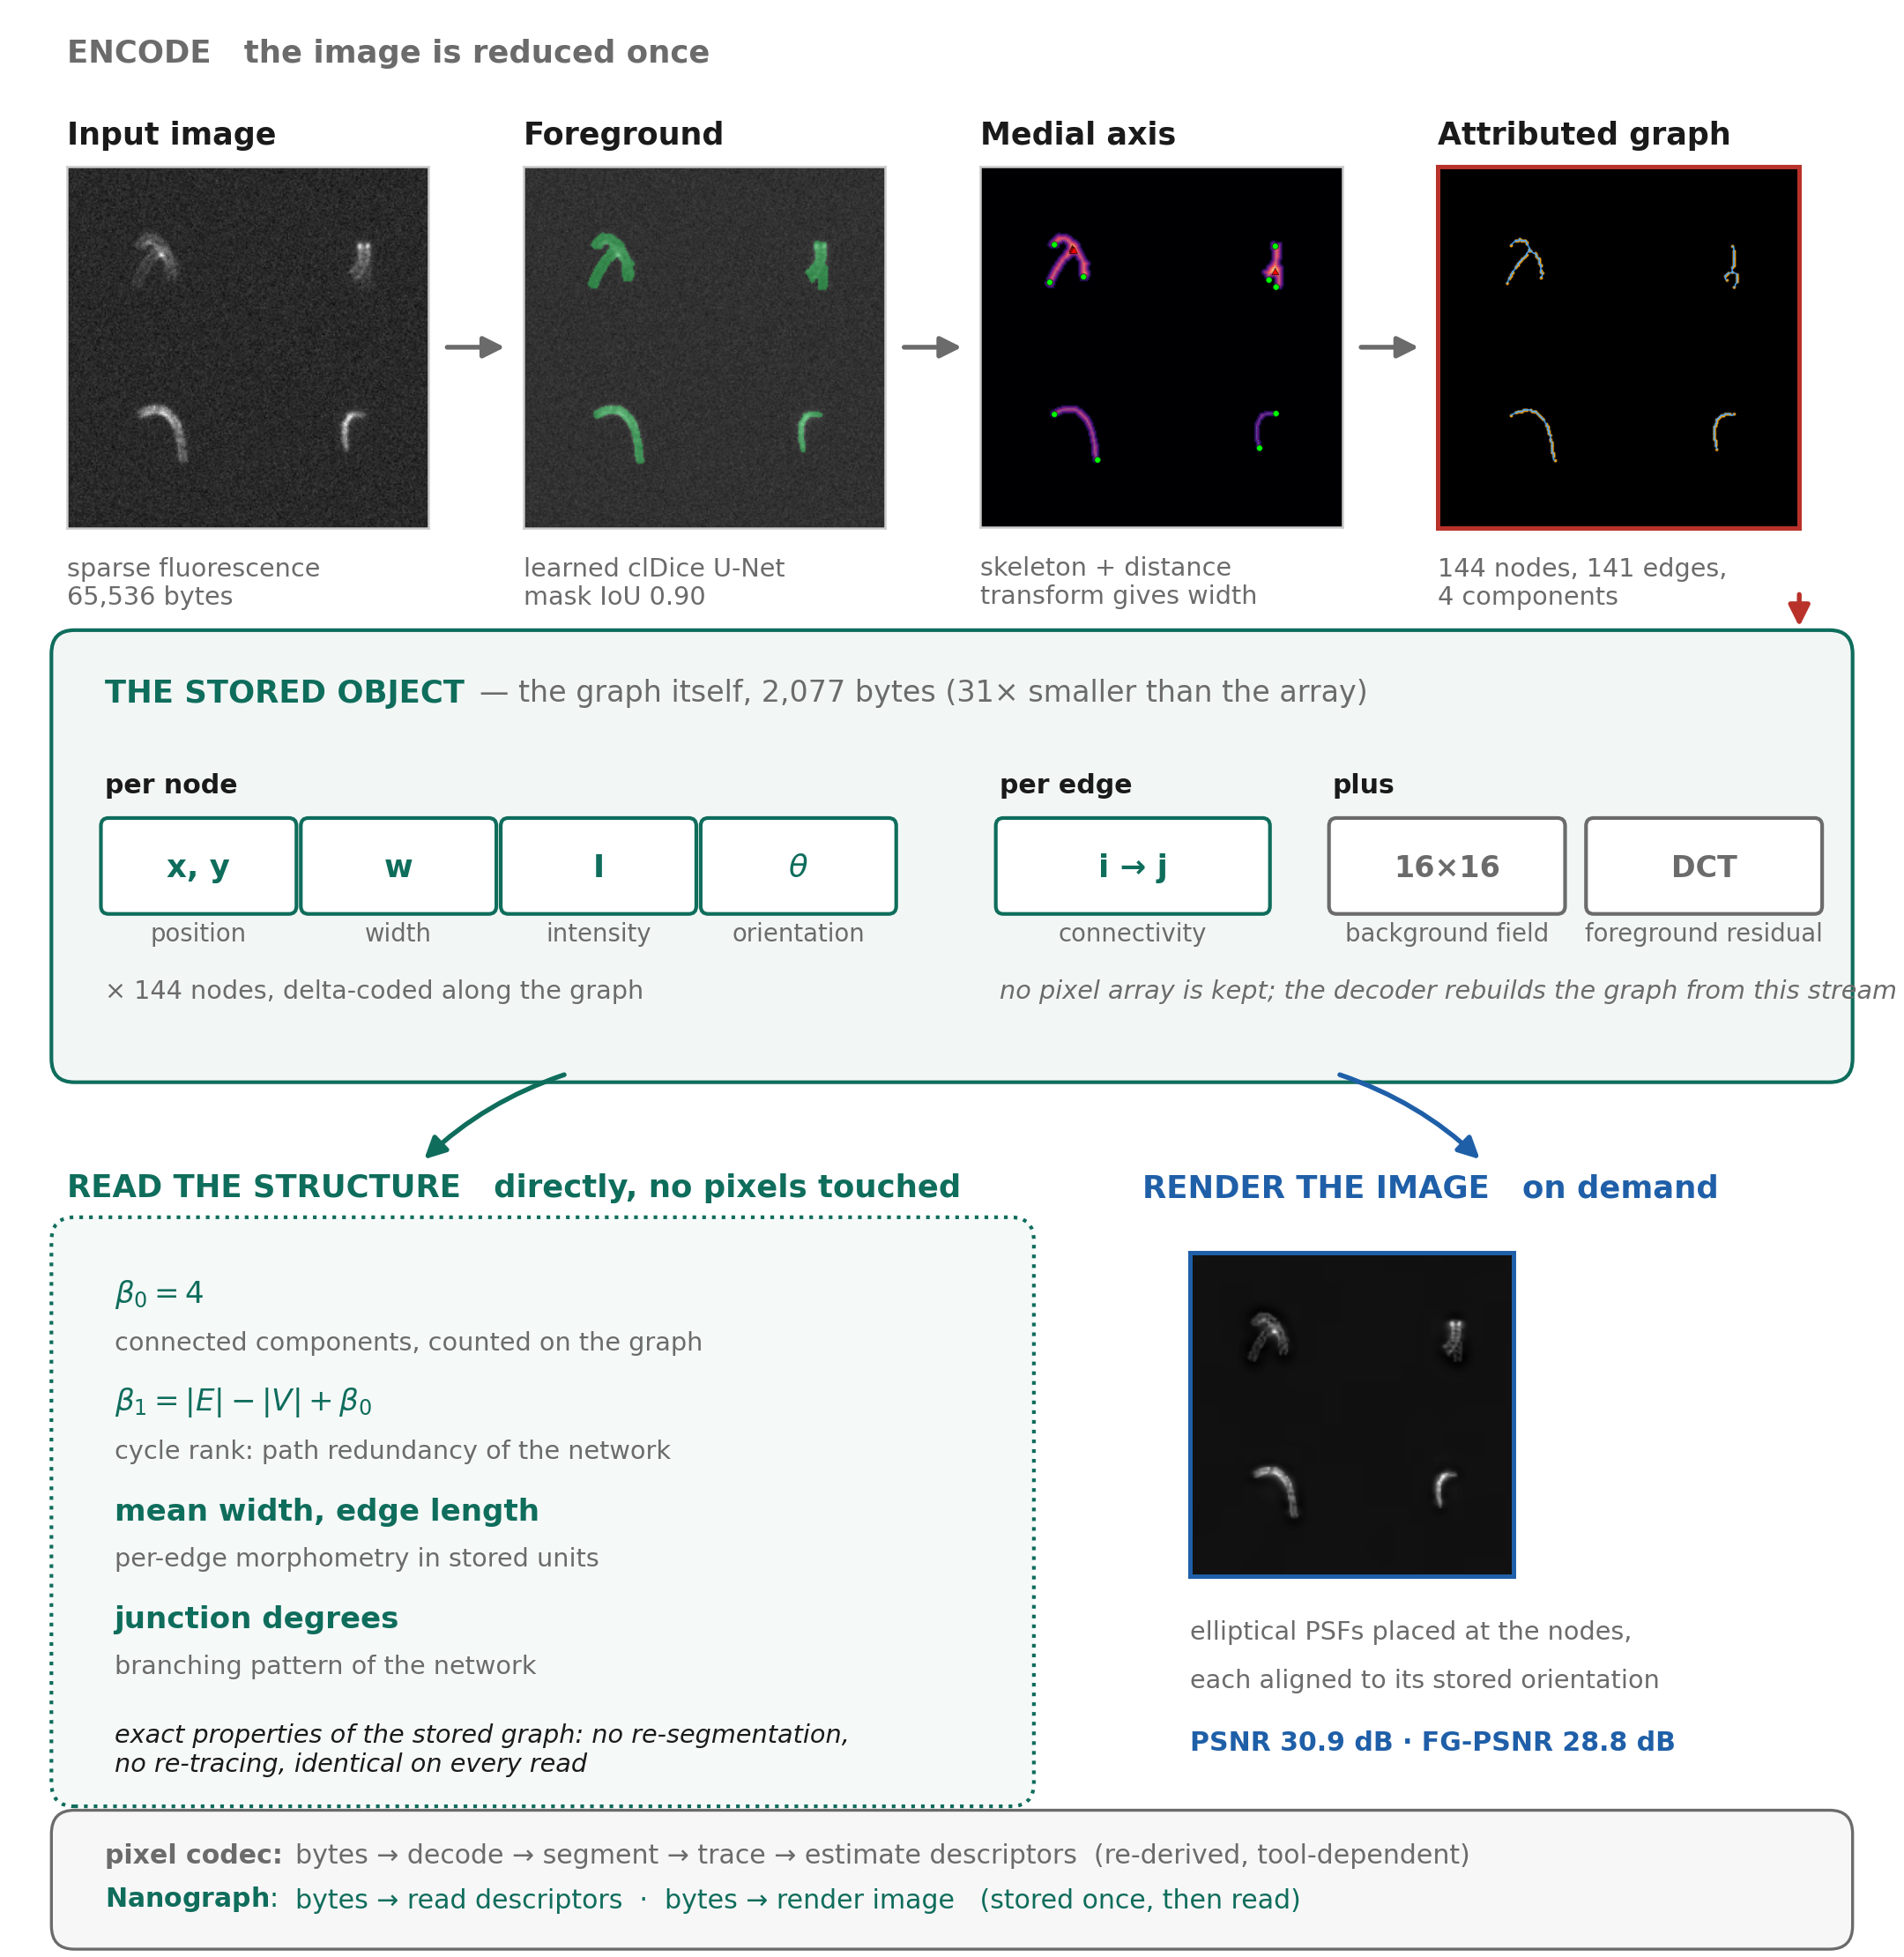
\includegraphics[width=0.92\textwidth]{figures/fig_pipeline.png}
\caption{\textbf{\method reduces a curvilinear image once, then reads the
result.} Top: the encode path, on a simulated fluorescence mitochondria image. Middle:
what is stored---the structure layer (branch polylines with width and path
length, junction nodes, connectivity) and the appearance layer (rendering
points with width, intensity and orientation, a coarse background field and
an optional foreground residual).
Bottom left: topology and morphometry are properties of that stored object
and are read from it without touching pixels. Bottom right: the image is
re-rendered on demand by placing orientation-aligned elliptical
point-spread functions at the nodes. A pixel codec must re-derive every
descriptor after decoding; \method stores them once.}
\label{fig:overview}
\end{figure}

\subsection{The structure layer is the analysis of the mask, at half its size}
\label{sec:layers}
The structure layer is designed to carry exactly what analysis needs. On the
726-image organelle set it takes $\StructBytesm$\,bytes per image, about
$\StructFracPct\%$ of the full payload ($\StructBytesm$ structure $+$
$\AppearBytesm$ appearance), and $\StructVsMaskX\times$ less than the same
segmentation mask stored losslessly as a bit-packed, zlib-compressed array
($\MaskLosslessBytesm$\,bytes; Fig.~\ref{fig:layers}). Splitting the payload
into two layers costs nothing: the appearance layer is the rendering stream
of the single-layer format, and the rendered images are identical.

What the structure layer stores is the analysis of the mask it encodes.
Built from a mask and decoded from its bytes, it reproduces the mask's
skeleton descriptors---components, branches, junctions, cycle rank, total
length and mean width---on every organelle image (Methods; a unit test
checks branch and junction counts against an independent skeleton analysis,
skan~\cite{skan}). Its topology agrees with the mask's own: the stored
component count equals the mask's $\beta_0$ on $\GraphCompEqPct\%$ of images,
and the stored cycle rank equals the mask's number of enclosed holes on
$\GraphCycEqPct\%$. An earlier builder that sampled nodes at fixed spacing
along skeleton pixels, which we keep as an ablation, matched on 95.6\% and
16\% of images: junction pixels produced spurious short cycles. A lossless
mask would carry the same information, but it must be re-skeletonised and
re-traced before every query. The structure layer is smaller, and the answer
is already in it.

\begin{figure}[t]
\centering
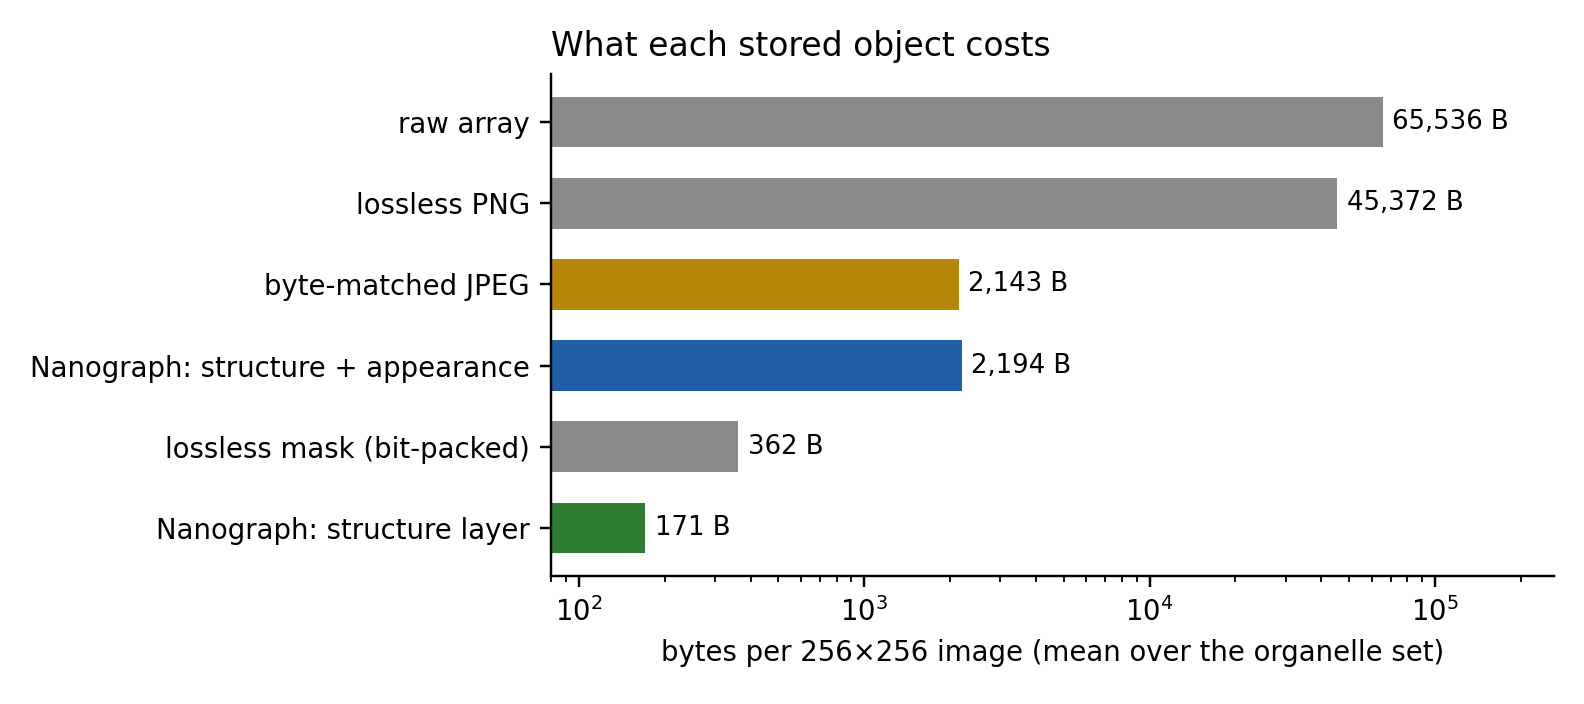
\includegraphics[width=0.8\textwidth]{figures/fig_layers.png}
\caption{\textbf{What each stored object costs} on the 726-image organelle
set (mean bytes per $256\times256$ image, log axis). The structure layer
alone supports every descriptor in this paper; the lossless mask carries the
same information but must be re-analysed before each query; the full
\method payload and a byte-matched JPEG are the two routes that also
regenerate the image.}
\label{fig:layers}
\end{figure}

\subsection{The graph costs the storage budget of an unstructured point set}
\label{sec:budget}
The storage cost of any key-point representation factorises as
\begin{equation}
\mathrm{BRR} \;=\; \underbrace{\mathrm{APRR}}_{\text{primitives per pixel}}
\times \underbrace{(\text{bytes per primitive})}_{\text{richness of each primitive}} ,
\label{eq:budget}
\end{equation}
where BRR is stored bytes per raw byte and APRR stored primitives per
pixel. Both are resolution-normalised, so they can be compared across the
compact-representation line even though the earlier systems were evaluated
on a different mitochondrial dataset~\cite{sekh2021}. Every earlier system,
and the classical skeleton, edge and boundary baselines, lands near
$\mathrm{BRR}\approx0.04$ with 1--4-byte coordinates (Table~\ref{tab:prior},
Fig.~\ref{fig:prior}). \method reaches the same band by the opposite route:
it stores \DFewerX$\times$ fewer primitives than GU-Net/GU-Net++, each
\DRicherX$\times$ richer ($\mathrm{BRR}=\DBRR$ vs.\ $0.0365$). The additional
bytes per primitive are what turn an unstructured point set into a queryable
structure, and they are paid for by storing fewer, better-placed
primitives.

\begin{table}[t]
\centering
\caption{\textbf{Storage across the compact-representation line.} APRR and
BRR are resolution-normalised. Prior-work values are as reported on
UiTMito~\cite{sekh2021} ($1024\times1024$); \method on the 726-image
organelle set ($256\times256$). Bytes per primitive is
$\mathrm{BRR}/\mathrm{APRR}$ (Eq.~\ref{eq:budget}).}
\label{tab:prior}
\footnotesize
\begin{adjustbox}{max width=\linewidth}
\begin{tabular}{llccc}
\toprule
System & Stored primitive & APRR $\downarrow$ & BRR $\downarrow$ & Bytes/prim.\\
\midrule
Skeleton~\cite{banerjee2024gunetpp}     & pixel coordinate & 0.0161 & 0.0321 & 2.0\\
Canny edge~\cite{banerjee2024gunetpp}   & pixel coordinate & 0.0203 & 0.0406 & 2.0\\
Boundary~\cite{banerjee2024gunetpp}     & pixel coordinate & 0.0295 & 0.0391 & 1.3\\
GA-CIR~\cite{malakar2025eaai}           & pixel coordinate & 0.0100 & 0.0400 & 4.0\\
GU-Net~\cite{banerjee2023acpr} / GU-Net++~\cite{banerjee2024gunetpp}
                                        & pixel coordinate & 0.0183 & 0.0365 & 2.0\\
\midrule
\method (this work) & graph node + width, intensity,
                                        & \textbf{\DAPRR} & \DBRR & \DBPP\\
                    & \quad orientation, edges & & & \\
\bottomrule
\end{tabular}
\end{adjustbox}
\end{table}

\begin{figure}[t]
\centering
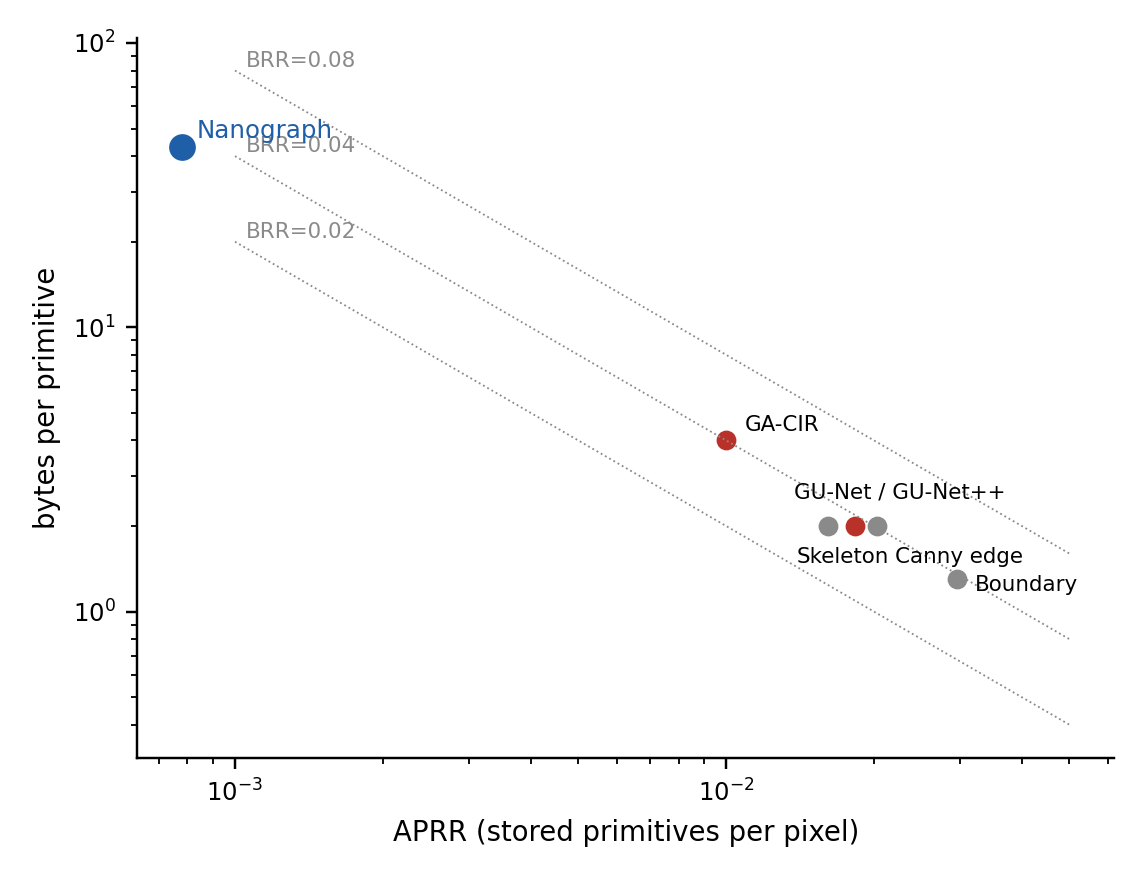
\includegraphics[width=0.62\textwidth]{figures/fig_prior_positioning.png}
\caption{\textbf{Same budget, spent differently.} Storage decomposes into how
many primitives are stored (APRR) and how rich each one is
(Eq.~\ref{eq:budget}); dotted lines are equal-storage contours. Our earlier
systems (red) and classical baselines (grey) sit near
$\mathrm{BRR}\approx0.04$ with 1--4-byte coordinates; \method (blue) stores
far fewer, far richer primitives.}
\label{fig:prior}
\end{figure}

\subsection{The stored graph exposes topology and morphometry directly}
\label{sec:yields}
On the 726-image organelle set each image is stored in
$\DBytesm$\,bytes, $\DVsRawm\times$ smaller than the raw array and
$\DVsPNGm\times$ smaller than lossless PNG (Table~\ref{tab:nmi}). The same
object answers structural queries directly: $\beta_0=\DBetaZero$
components, a cycle rank of $\DCycles$ (matching the mask's
$\beta_1=\DBetaOne$ enclosed holes), mean width $\DWidth$\,px and total
length (Fig.~\ref{fig:topology}), with no segmentation or tracing of pixels
at analysis time. The simulated tubes in this set are unbranched, so its
junctions and cycles arise only where tubes cross in projection; we show
branching-network statistics on real mitochondria below. Inside the
foreground the regenerated image is faithful (FG-SSIM $\DFGSSIM$;
GT-FG-SSIM $\DGTFGSSIM$ inside the simulator's ground-truth mask).
Full-image SSIM ($\DFullSSIMm$) reflects a deliberate design choice: the
noisy background of these sparse fields is summarised by a 256-byte field
rather than stored. Replacing the classical cascade by the learned front end
(Methods) raises Seg-IoU from $\CSegIoUm$ to $\DSegIoUm$ and produces
markedly cleaner graphs (cycle rank $\CCyclesm\to\DCyclesm$, mean width
$\CWidthm\to\DWidthm$\,px) at a smaller payload
($\CBytesm\to\DBytesm$\,bytes).

\begin{table}[t]
\centering
\caption{\textbf{\method on 726 organelle images} (mean$\pm$s.d.), with the
classical cascade and with the default learned front end. Metric
definitions are given in Methods.}
\label{tab:nmi}
\footnotesize
\begin{adjustbox}{max width=\linewidth}
\begin{tabular}{llcc}
\toprule
 & Quantity & Classical cascade & Default (learned front end)\\
\midrule
Storage   & Payload (bytes) & $\CBytes$ & $\DBytes$\\
          & Nodes / edges & $\CNodesm$ / $\CEdgesm$ & $\DNodesm$ / $\DEdgesm$\\
          & Reduction vs.\ raw / PNG ($\times$) & $\CVsRawm$ / $\CVsPNGm$ & $\DVsRawm$ / $\DVsPNGm$\\
          & Encode time (ms) & $\CTime$ & $\DTime$\\
\midrule
Segmentation & Seg-IoU (mask vs.\ GT) & $\CSegIoU$ & $\DSegIoU$\\
          & Precision / recall & $\CSegPrecm$ / $\CSegRecm$ & $\DSegPrecm$ / $\DSegRecm$\\
\midrule
Fidelity  & FG-PSNR (dB) / FG-SSIM & $\CFGPSNRm$ / $\CFGSSIMm$ & $\DFGPSNRm$ / $\DFGSSIMm$\\
          & GT-FG-PSNR (dB) / GT-FG-SSIM & $\CGTFGPSNRm$ / $\CGTFGSSIMm$ & $\DGTFGPSNRm$ / $\DGTFGSSIMm$\\
          & GT-IoU (reconstruction vs.\ GT) & $\CGTIoU$ & $\DGTIoU$\\
          & Full PSNR (dB) / SSIM & $\CFullPSNRm$ / $\CFullSSIMm$ & $\DFullPSNRm$ / $\DFullSSIMm$\\
\midrule
Structure & $\beta_0$ (components) & $\CBetaZero$ & $\DBetaZero$\\
          & $\beta_1$ (enclosed holes) & $\CBetaOne$ & $\DBetaOne$\\
          & Stored-graph cycle rank & $\CCycles$ & $\DCycles$\\
          & Mean width (px) & $\CWidth$ & $\DWidth$\\
\bottomrule
\end{tabular}
\end{adjustbox}
\end{table}

\begin{figure}[t]
\centering
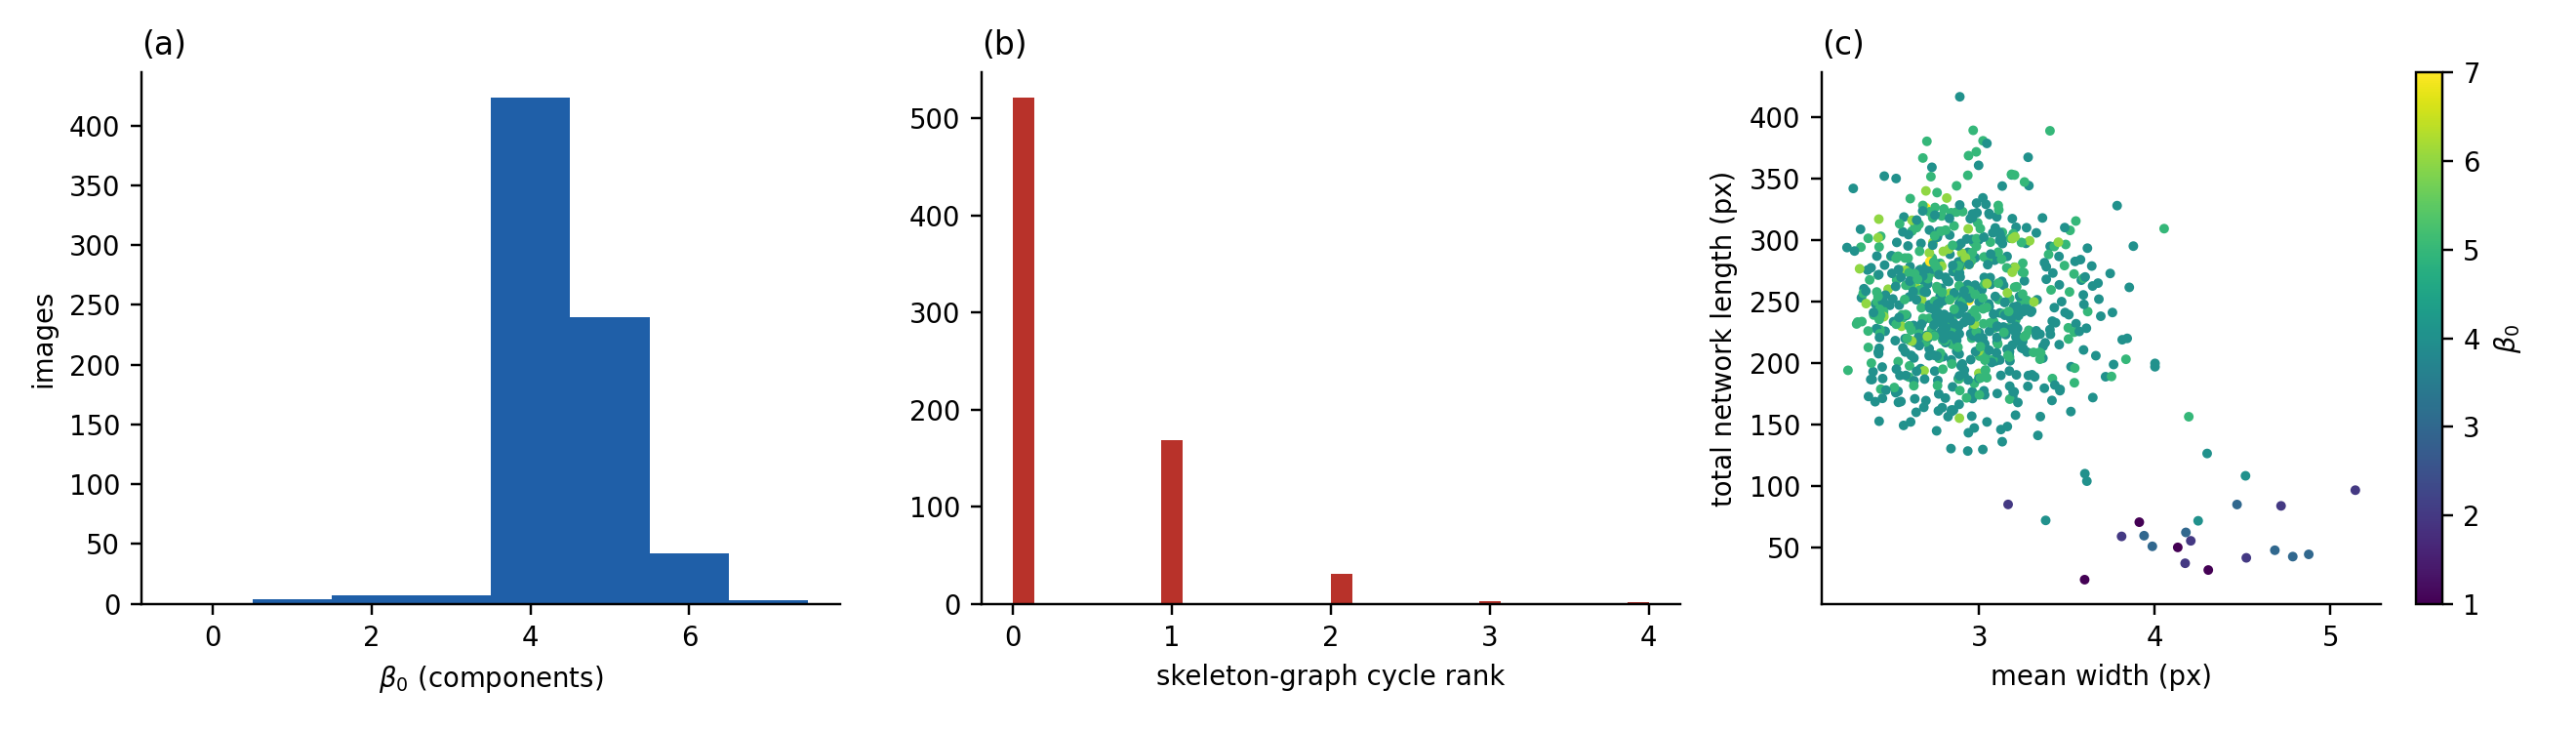
\includegraphics[width=\textwidth]{figures/fig_topology.png}
\caption{\textbf{Structural descriptors read directly from the stored
graph.} (a)~Components $\beta_0$. (b)~Cycle rank of the stored graph
(Methods); on these unbranched simulated tubes, cycles arise where tubes
cross in projection. (c)~Total length against mean width, coloured by
$\beta_0$.}
\label{fig:topology}
\end{figure}

\begin{figure}[t]
\centering
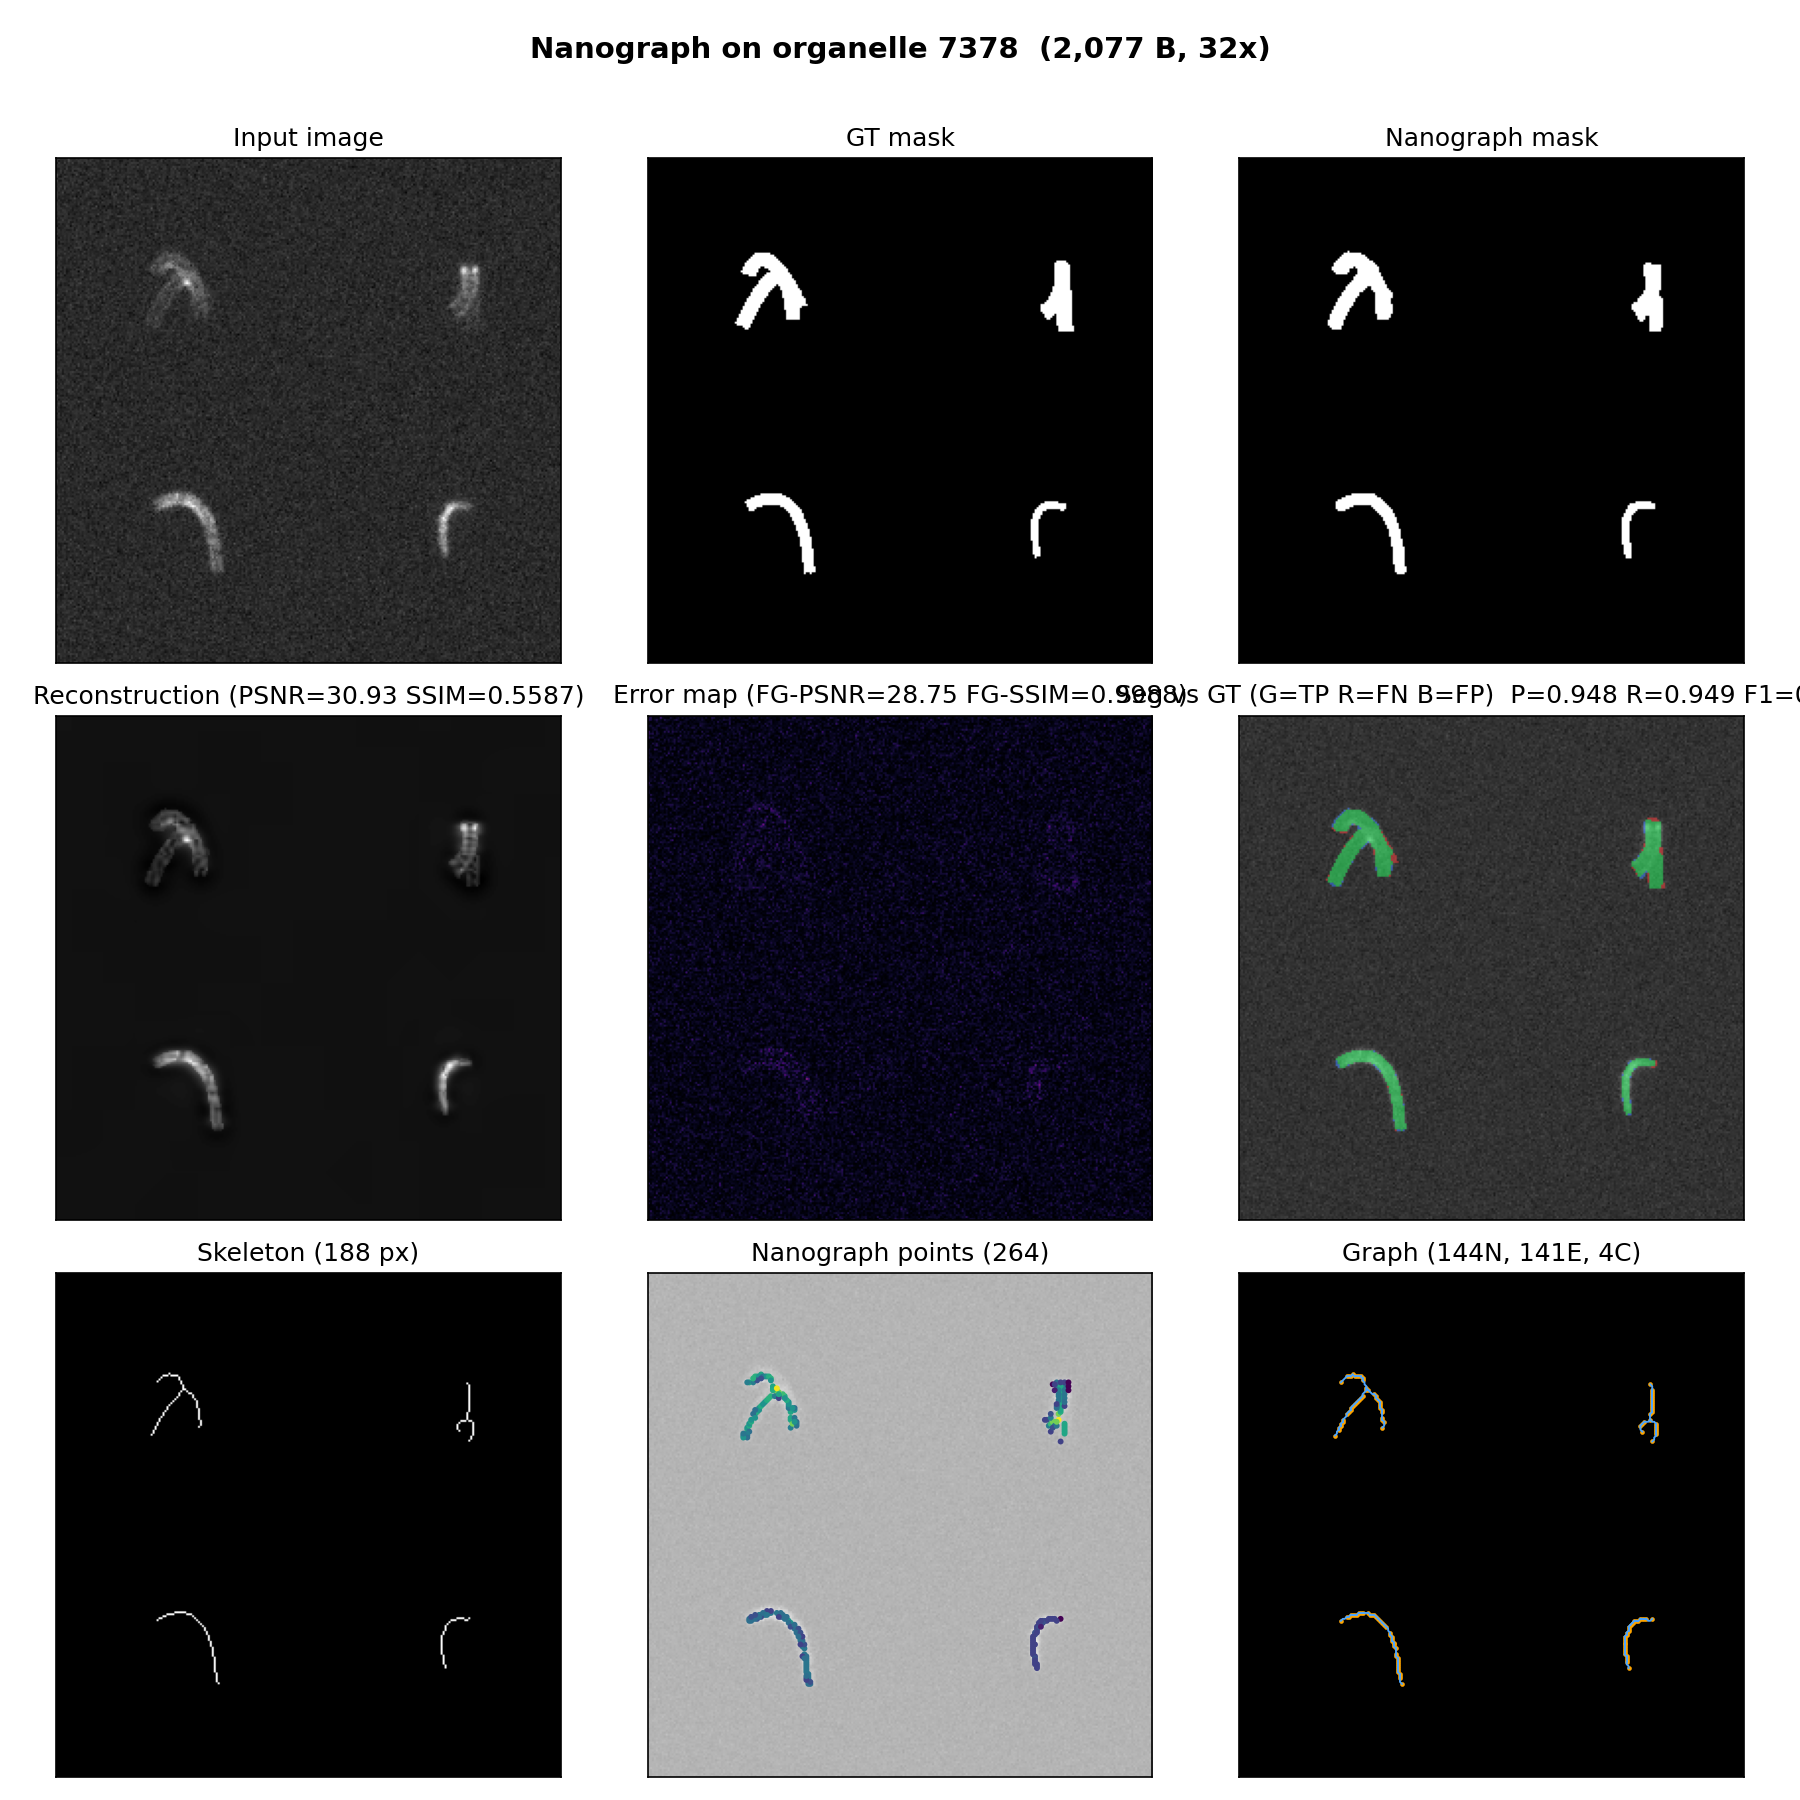
\includegraphics[width=0.92\textwidth]{figures/fig_qualitative_organelle.png}
\caption{\textbf{End-to-end example} on a held-out organelle image. Top row: input,
the segmentation mask selected by the cascade, and the simulator's
ground-truth mask. Middle row: oriented-PSF reconstruction from the graph,
absolute error map, and segmentation-vs-ground-truth overlay (green true
positive, red false negative, blue false positive). Bottom row: skeleton,
sampled graph nodes (red endpoints, blue junctions), and the final attributed
graph. The blue halo in the overlay is
the systematic over-prediction of the classical cascade quantified in
Fig.~\ref{fig:segbottleneck} (here precision 0.492 at recall 0.951).}
\label{fig:qualitative}
\end{figure}

\begin{figure}[t]
\centering
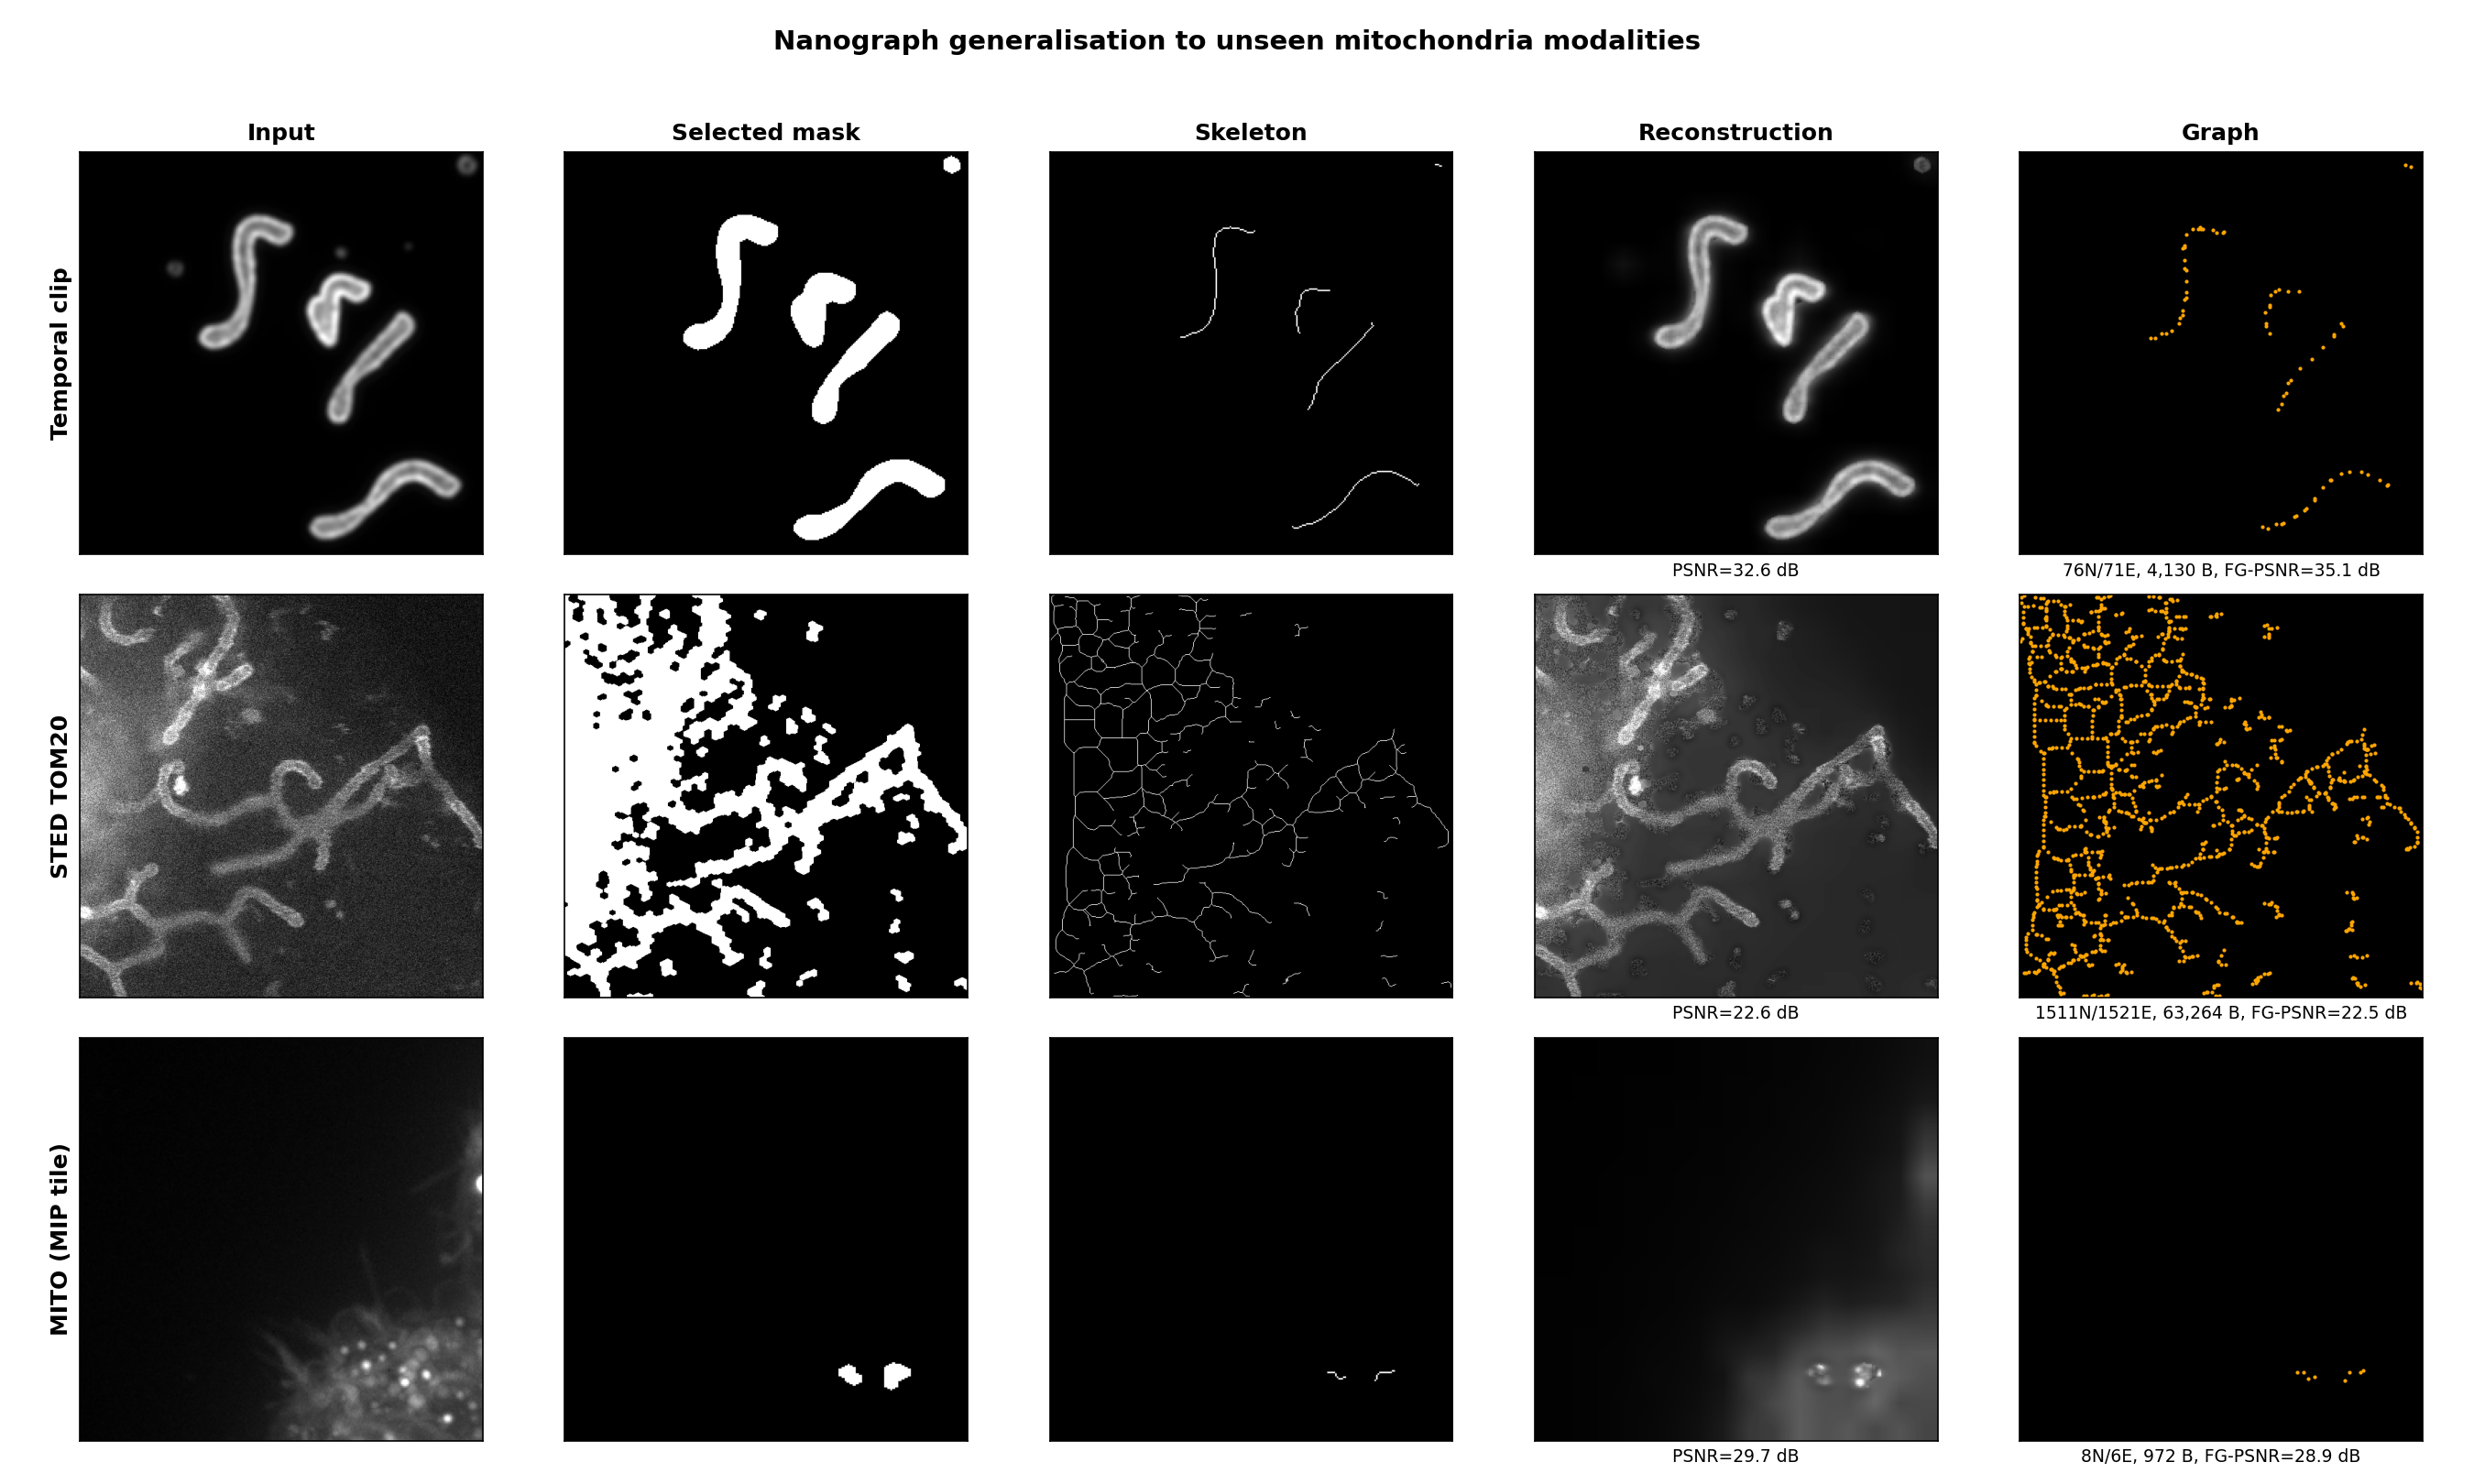
\includegraphics[width=\textwidth]{figures/fig_mito_generalisation.png}
\caption{\textbf{The same stages on three further mitochondrial
acquisitions} (input, selected mask, skeleton, reconstruction, graph nodes),
as a counterpart to Fig.~\ref{fig:qualitative}; the results are given in
Table~\ref{tab:mitogen} and discussed in the transfer section. Top: simulated temporal clip (four unbranched mitochondria in elastic motion; a separate dynamic simulator).
Middle: public live-cell STED (TOM20)~\cite{balakrishnan2024sted} with the
learned mask forced (\texttt{learned\_mode='replace'}); the outer-membrane
label makes tubes hollow, which the graph traces as parallel filaments.
Bottom: public confocal MITO dataset~\cite{zhanghao2023mito}, where the
selected mask covers less of the expert annotation.}
\label{fig:mitogen}
\end{figure}

\subsection{Analysis is read from the stored object}
\label{sec:downstream}
We next asked whether analysis read from the structure layer agrees with
analysis of the reference mask, and compared it with the route a pixel
archive offers: decode a byte-matched JPEG of the full payload, segment it
with the same learned segmenter, and analyse the result
(Table~\ref{tab:downstream}, Fig.~\ref{fig:downstream}; Methods). Every arm
passes through one descriptor definition and one cleanup rule. Terminal
branches and isolated fragments shorter than one mean structure diameter are
removed (the \emph{one-diameter rule}). The rule was fixed before any
comparison with the simulated ground truth, has no free parameter, and is
applied at analysis time, so the stored payload is unchanged. Fixed lengths
of 0, 2, 5 and 10\,px are reported in the Supplement.

Across \DsN{} organelle images the stored graph agrees with the reference
mask more closely than the byte-matched JPEG route on every descriptor
(Table~\ref{tab:downstream}). The difference is largest for the counts.
Re-segmenting a JPEG fragments thin tubes at block boundaries, which adds
components and short branches (components $\DsPJpegNComponentsBiasPct\%$,
CCC $\DsPJpegNComponentsCCC$). The stored graph inherits only the
segmenter's own error on the original image (components
$\DsPGraphNComponentsBiasPct\%$, CCC $\DsPGraphNComponentsCCC$). The
branch-length distribution is also closer to the reference (mean
Wasserstein distance $\DsPWassGraph$ vs.\ $\DsPWassJpeg$\,px). Reading the
descriptors takes $\DsTimeGraph$\,ms per image from the payload, against
$\DsTimeRef$\,ms to re-analyse a stored mask and $\DsTimeJpeg$\,ms to
decode, segment and skeletonise a JPEG (single thread; Methods).

\begin{table}[t]
\centering
\caption{\textbf{Descriptors read from the stored graph vs.\ a byte-matched
JPEG route}, each compared with the same descriptors of the reference mask
(726 organelle images, one-diameter rule in every arm). CCC: Lin's
concordance; MdAPE: median absolute percentage error; bias: mean relative
error. Last column: images on which the stored graph is closer to the
reference than JPEG, with paired Wilcoxon $p$.}
\label{tab:downstream}
\footnotesize
\setlength{\tabcolsep}{3.5pt}
\begin{adjustbox}{max width=\linewidth}
\begin{tabular}{lccccccc}
\toprule
 & \multicolumn{3}{c}{\method structure layer} & \multicolumn{3}{c}{byte-matched JPEG} & \\
\cmidrule(lr){2-4}\cmidrule(lr){5-7}
Descriptor & CCC & MdAPE (\%) & Bias (\%) & CCC & MdAPE (\%) & Bias (\%) & Graph closer\\
\midrule
Components & $\DsPGraphNComponentsCCC$ & $\DsPGraphNComponentsMdAPE$ & $\DsPGraphNComponentsBiasPct$ & $\DsPJpegNComponentsCCC$ & $\DsPJpegNComponentsMdAPE$ & $\DsPJpegNComponentsBiasPct$ & \DsPWinsNComponents ($p=\DsPWinsPNComponents$)\\
Total length & $\DsPGraphTotalLengthCCC$ & $\DsPGraphTotalLengthMdAPE$ & $\DsPGraphTotalLengthBiasPct$ & $\DsPJpegTotalLengthCCC$ & $\DsPJpegTotalLengthMdAPE$ & $\DsPJpegTotalLengthBiasPct$ & \DsPWinsTotalLength ($p=\DsPWinsPTotalLength$)\\
Mean width & $\DsPGraphMeanWidthCCC$ & $\DsPGraphMeanWidthMdAPE$ & $\DsPGraphMeanWidthBiasPct$ & $\DsPJpegMeanWidthCCC$ & $\DsPJpegMeanWidthMdAPE$ & $\DsPJpegMeanWidthBiasPct$ & \DsPWinsMeanWidth ($p=\DsPWinsPMeanWidth$)\\
Branches & $\DsPGraphNBranchesCCC$ & $\DsPGraphNBranchesMdAPE$ & $\DsPGraphNBranchesBiasPct$ & $\DsPJpegNBranchesCCC$ & $\DsPJpegNBranchesMdAPE$ & $\DsPJpegNBranchesBiasPct$ & \DsPWinsNBranches ($p=\DsPWinsPNBranches$)\\
Junctions & $\DsPGraphNJunctionsCCC$ & $\DsPGraphNJunctionsMdAPE$ & $\DsPGraphNJunctionsBiasPct$ & $\DsPJpegNJunctionsCCC$ & $\DsPJpegNJunctionsMdAPE$ & $\DsPJpegNJunctionsBiasPct$ & \DsPWinsNJunctions ($p=\DsPWinsPNJunctions$)\\
Cycle rank & $\DsPGraphCycleRankCCC$ & $\DsPGraphCycleRankMdAPE$ & $\DsPGraphCycleRankBiasPct$ & $\DsPJpegCycleRankCCC$ & $\DsPJpegCycleRankMdAPE$ & $\DsPJpegCycleRankBiasPct$ & \DsPWinsCycleRank ($p=\DsPWinsPCycleRank$)\\
\bottomrule
\end{tabular}
\end{adjustbox}
\end{table}

\begin{figure}[t]
\centering
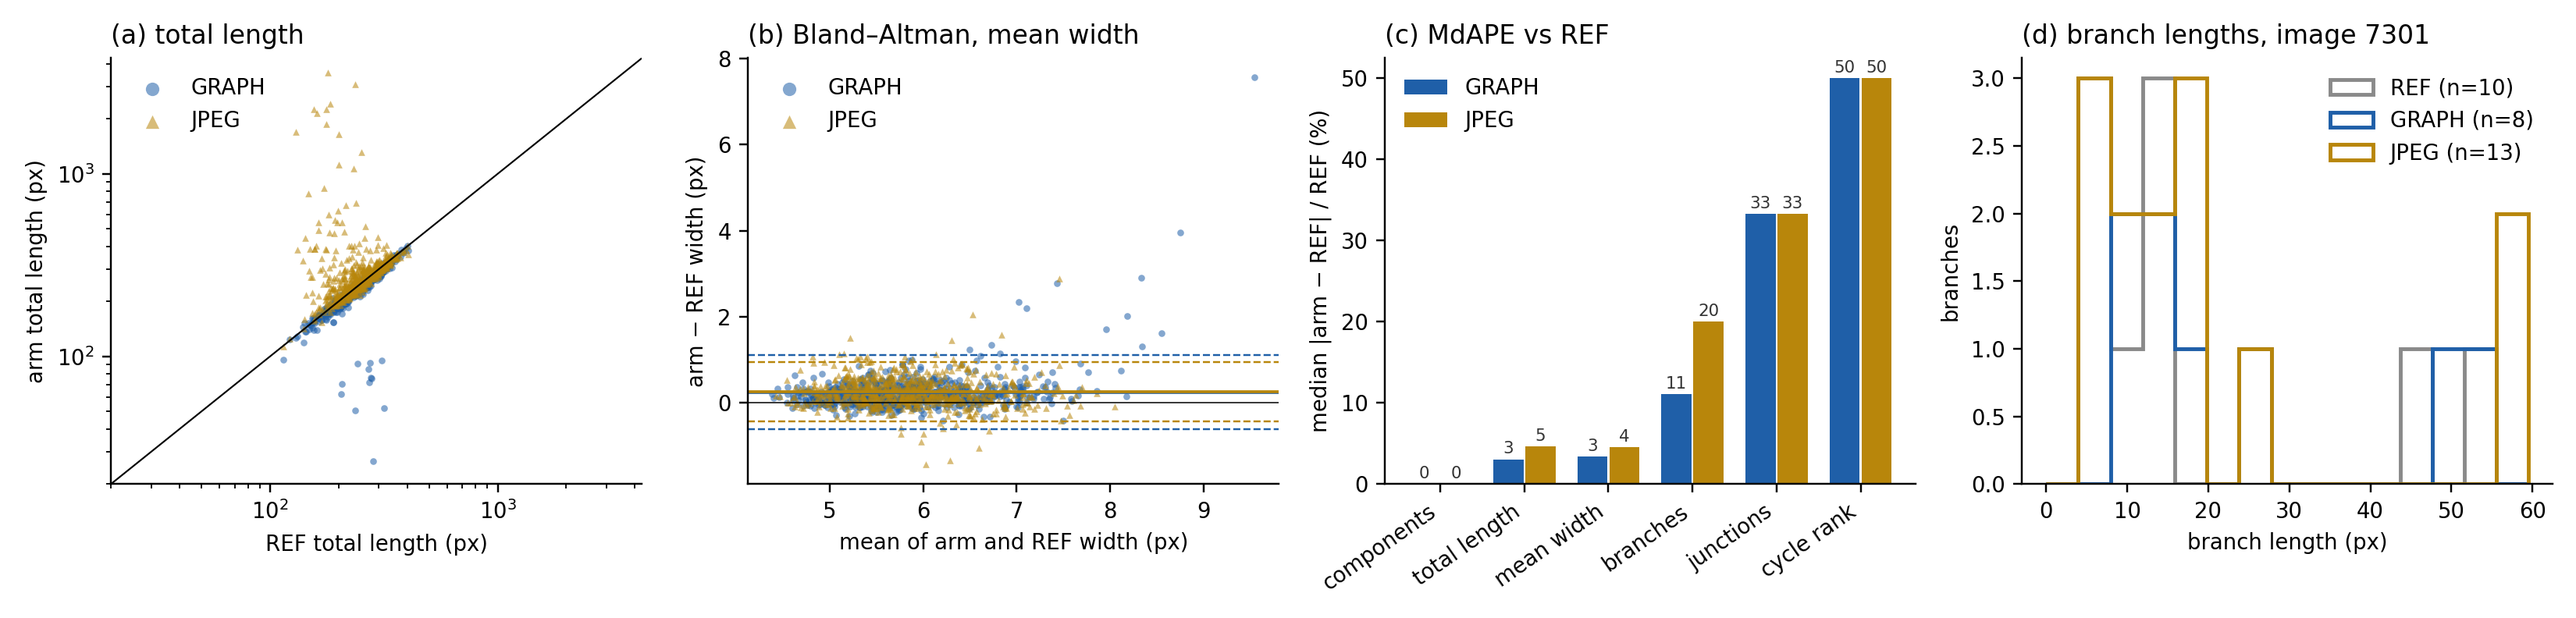
\includegraphics[width=\textwidth]{figures/fig_downstream.png}
\caption{\textbf{Descriptors read from the stored graph (GRAPH) and from a
re-segmented byte-matched JPEG, against the reference mask (REF).}
(a)~Total length per image (log axes). (b)~Bland--Altman plot of mean
width. (c)~Median absolute percentage error per descriptor. (d)~Branch-length
distributions on the image with the median GRAPH--REF Wasserstein distance.
One-diameter rule in every arm.}
\label{fig:downstream}
\end{figure}

\subsection{Against the true geometry}
\label{sec:truth}
A reference mask is itself a measurement. Simulation lets us compare every
route with the geometry that generated the image. We regenerated
\TruthN{} organelle-like images with the same simulator and settings,
keeping each tube's centreline and diameter (on average \TruthTubesm{}
tubes, \TruthCompm{} connected structures and \TruthJuncm{} projected
crossings per image; Methods), and measured three routes against it: the
simulator's own mask, the \method structure layer, and the byte-matched JPEG
route (Fig.~\ref{fig:truth}).

No 2-D route recovers the true geometry without bias, the simulator's own
mask included. At 42\,nm pixels, tubes of 20--300\,nm diameter are blurred
into structures of a few pixels, so the mask loses
$\TruthRefLenBias\%$ of the length and overstates width by
$\TruthRefWidthBias\%$; the stored graph inherits these biases
(length $\TruthGraphLenBias\%$, width $\TruthGraphWidthBias\%$).
JPEG's mean length bias ($\TruthJpegLenBias\%$) looks better, but it comes
from two errors cancelling: fragmentation adds length and merging removes
it, and its per-image concordance with the truth is low (CCC
$\TruthJpegLenCCC$ vs.\ $\TruthGraphLenCCC$). A consistent bias can be
calibrated out, and a random error cannot. After a two-fold cross-validated
linear calibration against the truth, the stored graph is as close to the
true geometry as the simulator's own mask. It is closer than the JPEG route
on components ($\CalGraphComp$ vs.\ $\CalJpegComp\%$ median error), length
($\CalGraphLen$ vs.\ $\CalJpegLen\%$), branches ($\CalGraphBr$ vs.\
$\CalJpegBr\%$) and junctions ($\CalGraphJunc$ vs.\ $\CalJpegJunc\%$;
Fig.~\ref{fig:truth}b).

The simulated temporal clip (73 frames, four unbranched mitochondria in
elastic motion, per-frame ground-truth skeletons~\cite{cods}) shows the
failure mode the one-diameter rule addresses (Fig.~\ref{fig:clip}). As the
mitochondria move and thin, segmentation leaves small fragments that a
count reads as extra mitochondria: without cleanup the stored graph
overcounts components by $\ClipTruthCompZero\%$, and with the one-diameter
rule by $\ClipTruthCompAuto\%$. Length is under-estimated by
$\ClipTruthLenAuto\%$ in the late frames, where the tubes approach the
optical limit.

\begin{figure}[t]
\centering
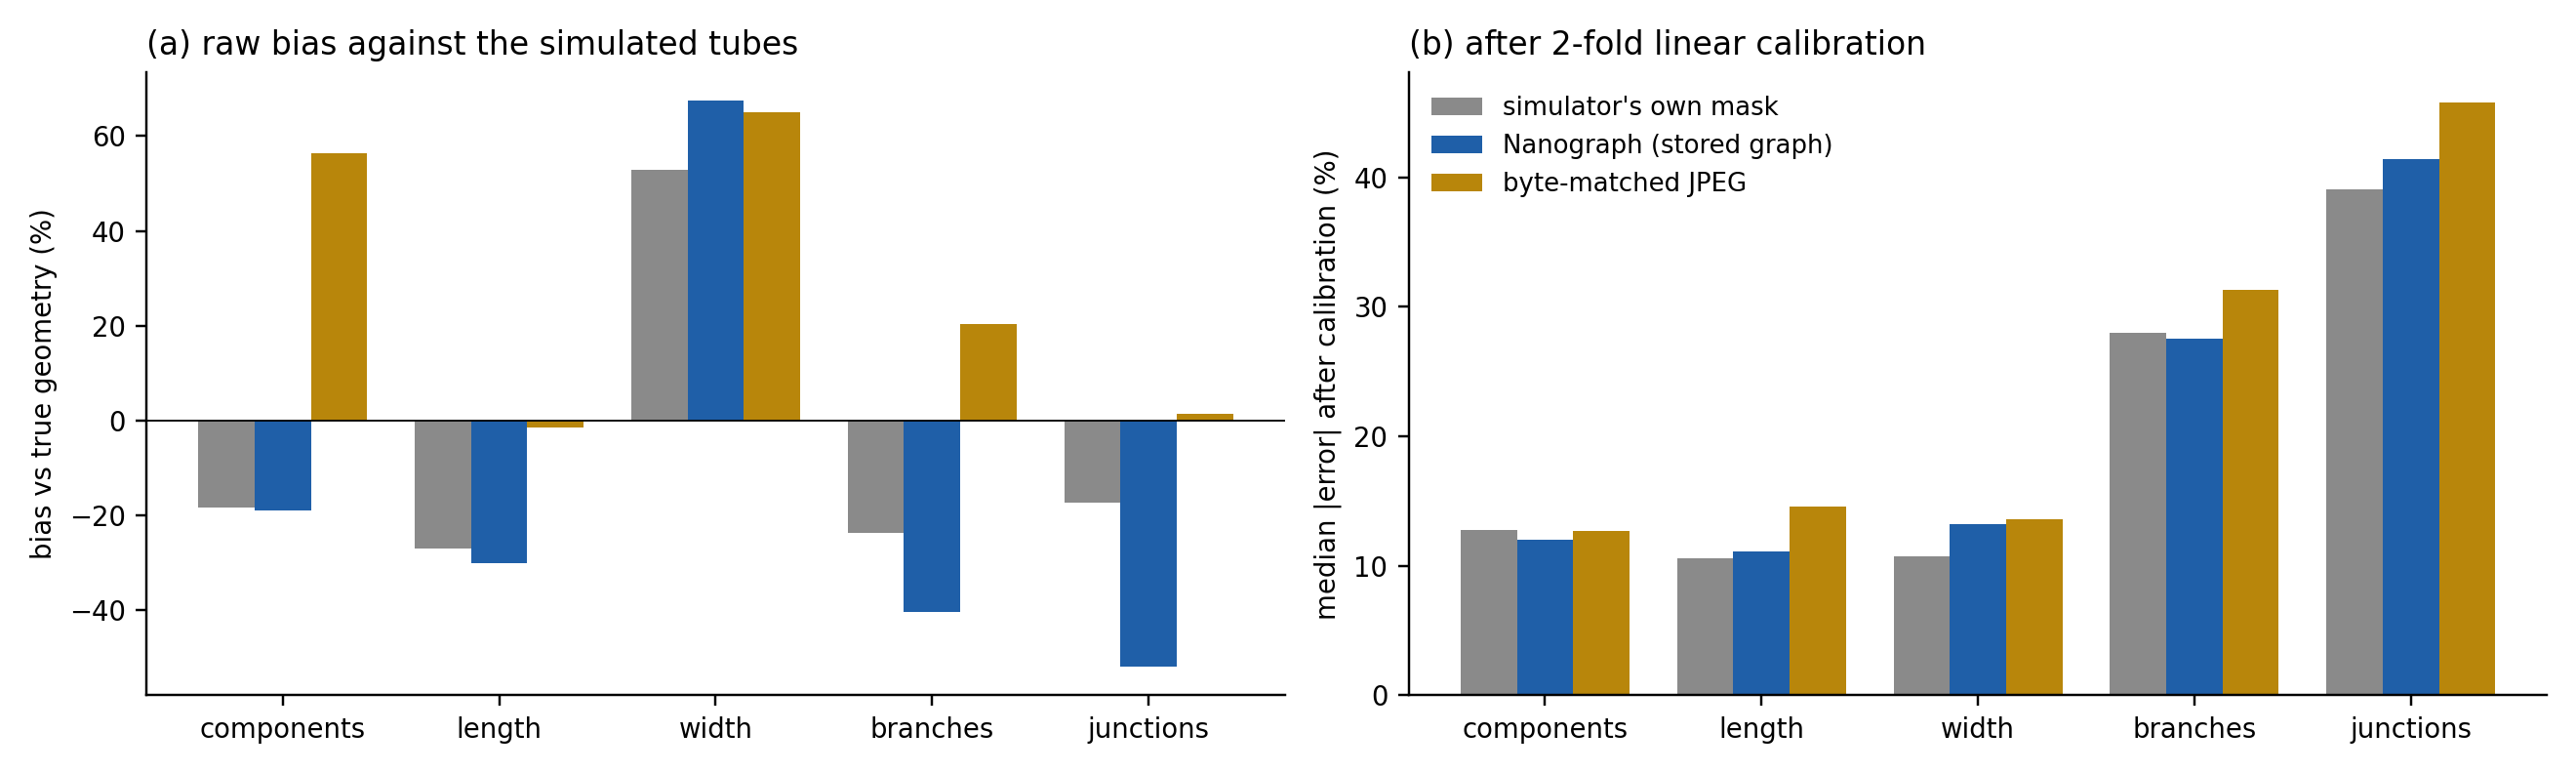
\includegraphics[width=\textwidth]{figures/fig_truth.png}
\caption{\textbf{Against the true simulated geometry} (\TruthN{} images).
(a)~Mean relative bias of each descriptor for the simulator's own mask, the
\method structure layer and the byte-matched JPEG route. (b)~Median absolute
error after two-fold cross-validated linear calibration against the truth.}
\label{fig:truth}
\end{figure}

\begin{figure}[t]
\centering
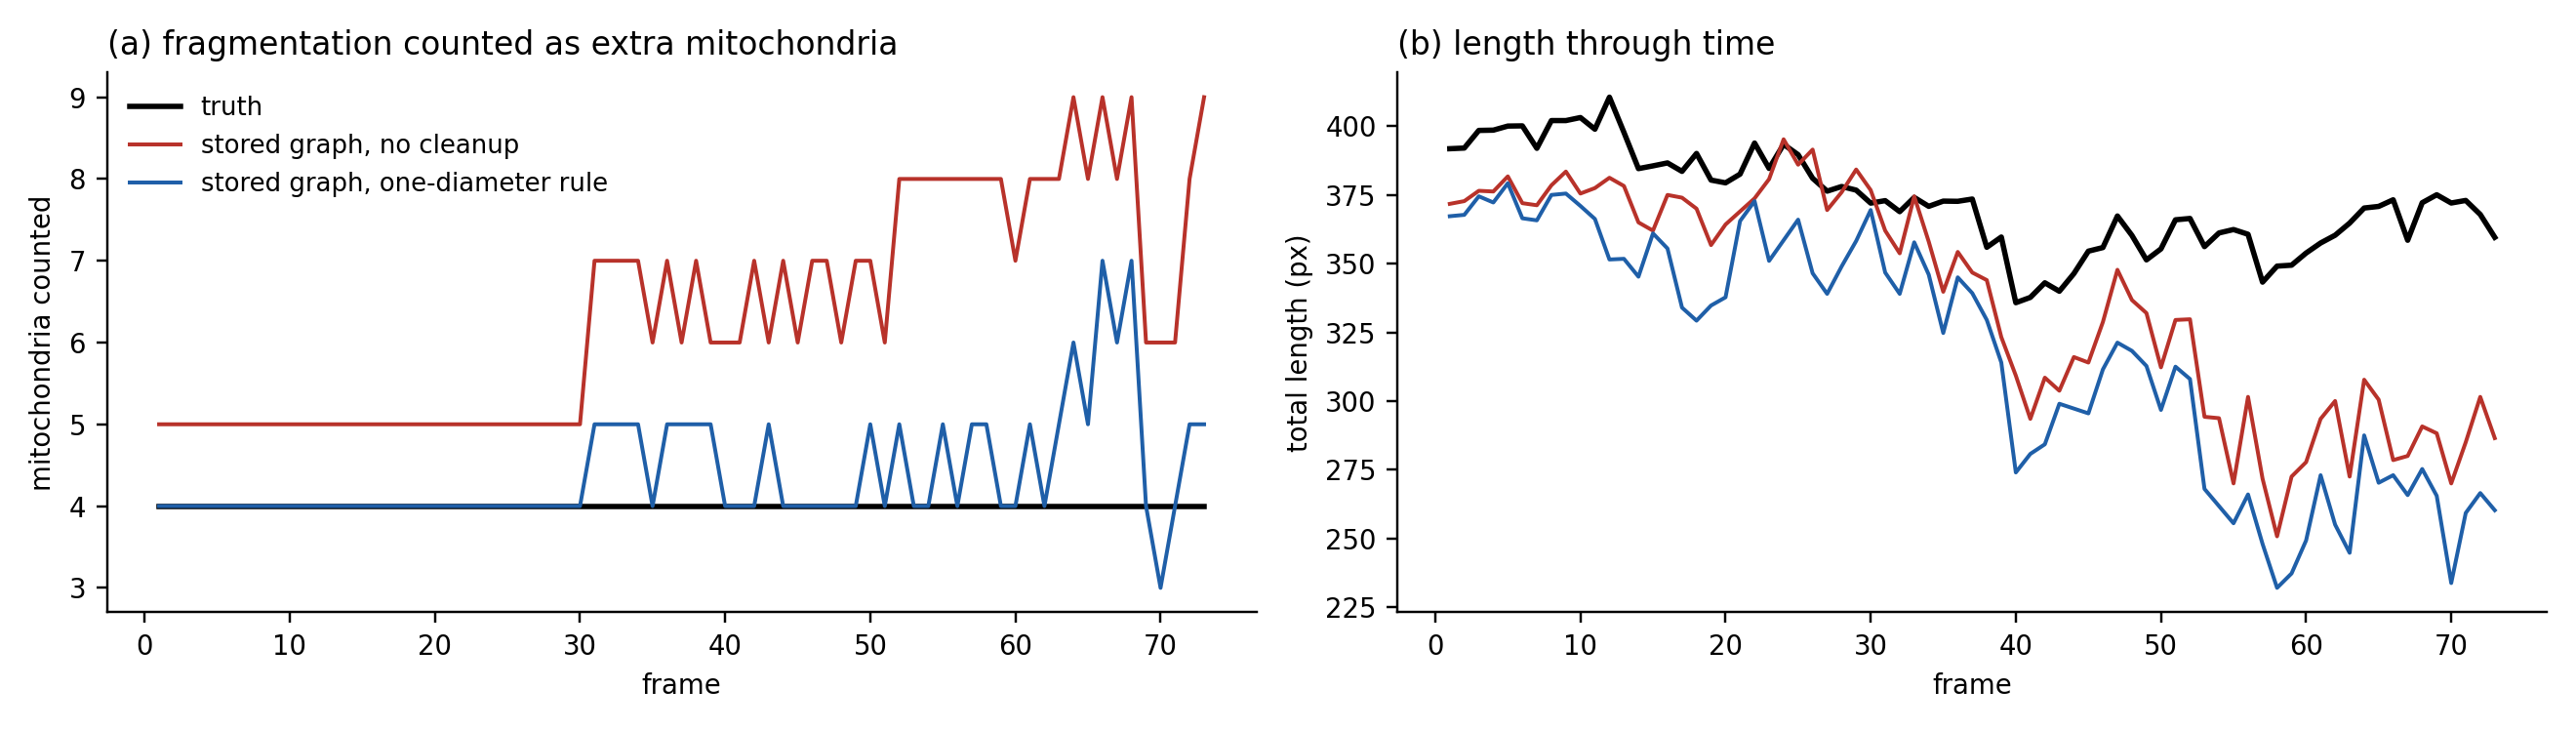
\includegraphics[width=\textwidth]{figures/fig_clip.png}
\caption{\textbf{The simulated temporal clip against its ground-truth
skeletons.} (a)~Number of mitochondria counted per frame from the stored
graph, without cleanup and with the one-diameter rule. (b)~Total length per
frame.}
\label{fig:clip}
\end{figure}

\subsection{Real mitochondria}
\label{sec:real}
We evaluated four real, expert-annotated mitochondrial datasets: UiT rat cells
(EP1-UiT-Rat, epifluorescence), CBMI~\cite{cbmi},
MITO~\cite{zhanghao2023mito} and UiT human cells (EP-UiT-Human), split by
frame or cell and never by tile (Methods). The organelle segmenter, trained
only on simulations, transfers poorly: in-pipeline Seg-IoU is
$\RealSegIoUSimUit$, $\RealSegIoUSimCbmi$, $\RealSegIoUSimMito$ and
$\RealSegIoUSimHuman$. We retrained it on the real training splits in
three ways---from scratch, fine-tuned from the simulation network, and jointly
with the simulations---with three seeds each, and additionally left each
dataset out of training in turn (36 networks; Table~\ref{tab:realseg}). The
joint network, which we ship as the \texttt{real-mito} preset, raises
in-pipeline Seg-IoU to $\RealSegIoURealUit$, $\RealSegIoURealCbmi$,
$\RealSegIoURealMito$ and $\RealSegIoURealHuman$ (Fig.~\ref{fig:real}a).
EP-UiT-Human was never used for training or model selection. On it, real
training mostly fixes topology: the branch-count bias falls from
$\RealHumanBrBiasSim\%$ to $\RealHumanBrBiasReal\%$ and its concordance
rises from $\RealHumanBrCCCSim$ to $\RealHumanBrCCCReal$. Transfer between
microscopes is limited. A network that has not seen a dataset's microscope
gains little on it (last row of Table~\ref{tab:realseg}), and on CBMI no
real-trained network improves on the simulation network by more than a few
points of IoU. Each new acquisition
type should therefore contribute training data.

On these data the structure layer takes
$\RealStructBytesMin$--$\RealStructBytesMax$\,bytes per $256\times256$ tile
(Fig.~\ref{fig:real}b). To support analysis from a pixel archive instead, a
JPEG must be decoded and re-segmented with the same network. Even the
smallest JPEG (quality 1, $\RealJpegQoneBytesUit$\,bytes on UiT) is
markedly worse. Branch-count concordance with the expert masks is
$\RealJpegQoneBrCCCUit$ vs.\ $\RealBrCCCUit$ for the structure layer on UiT,
and $\RealJpegQoneBrCCCHuman$ vs.\ $\RealBrCCCHuman$ on EP-UiT-Human.
At quality 20, which costs $\RealJpegRatioMin$--$\RealJpegRatioMax\times$
the bytes of the structure layer, JPEG reaches the structure layer's
concordance on CBMI and MITO, where every route is limited by segmentation
(branch CCC $\RealBrCCCCbmi$ and $\RealBrCCCMito$), and still falls short on
UiT and EP-UiT-Human. When JPEG is
instead given the full \method payload (4--6.5\,kB on these data, structure
plus appearance), it is close to lossless. Its analysis then matches
analysis of the original image, and the two routes tie within noise. At
that budget the structure layer reaches the same analysis from about a
tenth of the bytes, and needs no re-segmentation.

\begin{table}[t]
\centering
\caption{\textbf{Standalone segmentation of real mitochondria} (test-set
IoU against expert masks, mean over three seeds). EP-UiT-Human was used
neither for training nor for model selection; the last two columns give the
branch-count bias and concordance on it. Last row: each dataset's IoU from
the joint network trained without that dataset.}
\label{tab:realseg}
\footnotesize
\setlength{\tabcolsep}{4pt}
\begin{adjustbox}{max width=\linewidth}
\begin{tabular}{lcccccc}
\toprule
Training & UiT rat & CBMI & MITO & UiT human & Human branch bias & Human branch CCC\\
\midrule
\tabinput{tables/tab_realseg_body.tex}
\bottomrule
\end{tabular}
\end{adjustbox}
\end{table}

\begin{figure}[t]
\centering
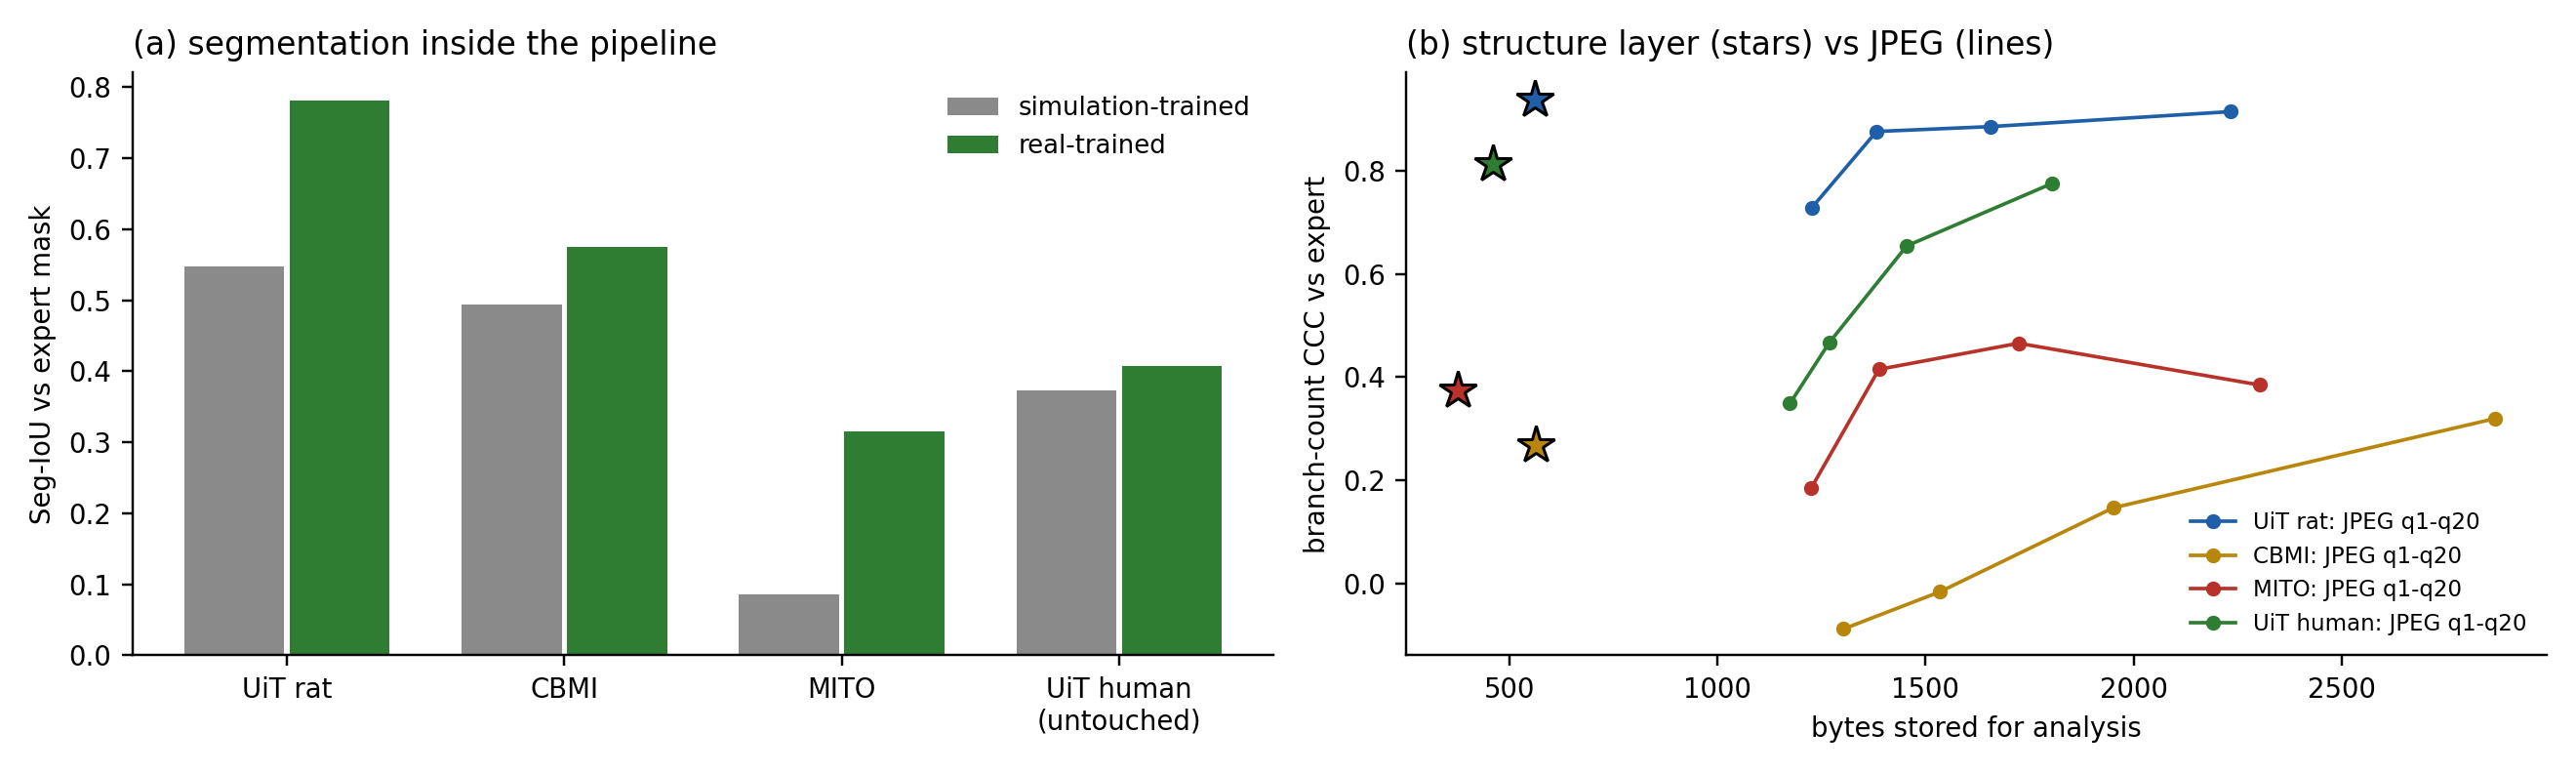
\includegraphics[width=\textwidth]{figures/fig_real.png}
\caption{\textbf{Real mitochondria.} (a)~In-pipeline Seg-IoU against the
expert masks with the simulation-trained and the real-trained
(\texttt{real-mito}) front end; EP-UiT-Human was untouched by training.
(b)~Branch-count concordance with the expert masks against bytes stored for
analysis: the \method structure layer (stars) and JPEG at quality 1--20,
decoded and re-segmented with the same network (lines).}
\label{fig:real}
\end{figure}

\subsection{Background-field and residual coding carry most of the foreground fidelity}
\label{sec:ablation}
Beyond node-level PSF placement, reconstruction includes a $16\times16$
background field and an optional DCT foreground residual. Encoding every
organelle image with and without both components shows that together they
add $\AblFGPSNRDeltam$\,dB FG-PSNR ($\AblFGPSNRWithoutm\to\AblFGPSNRWithm$\,dB,
improved on \AblImproved{} images), raise FG-SSIM from $\AblFGSSIMWithoutm$ to
$\AblFGSSIMWithm$ and full-image PSNR by $\AblFullPSNRDeltam$\,dB, at
$\AblBytesRatio\times$ the payload (Table~\ref{tab:ablation}). This is the
largest fidelity contribution of any single component.

\begin{table}[t]
\centering
\caption{\textbf{Background-field and residual coding} over the 726-image
organelle set (mean$\pm$s.d.; paired encodes differing only in the two
components).}
\label{tab:ablation}
\footnotesize
\begin{tabular}{lccc}
\toprule
 & Without & With & Paired $\Delta$\\
\midrule
FG-PSNR (dB)   & $\AblFGPSNRWithout$ & $\AblFGPSNRWith$ & $\AblFGPSNRDelta$\\
FG-SSIM        & $\AblFGSSIMWithout$ & $\AblFGSSIMWith$ & $\AblFGSSIMDeltam$\\
Full PSNR (dB) & $\AblFullPSNRWithout$ & $\AblFullPSNRWith$ & $\AblFullPSNRDelta$\\
Bytes          & $\AblBytesWithout$ & $\AblBytesWith$ & $\AblBytesRatio\times$\\
\bottomrule
\end{tabular}
\end{table}

\subsection{The same encoder transfers across five modalities}
\label{sec:cross}
Applied unchanged to Cells3D membrane and nuclei, retinal vessels and
fluorescence cells, the encoder keeps foreground fidelity high (FG-SSIM
0.97--0.99; Table~\ref{tab:cross}). Full-image fidelity is higher than on
organelles because these images have simpler backgrounds, which the
background field captures well. Payload scales with the structure rather
than with the frame: pooled over five modalities, bytes track skeleton-graph
cycle rank across two orders of magnitude (Fig.~\ref{fig:scaling}a), the
defining property of a structure-proportional representation.

\begin{table}[t]
\centering
\caption{\textbf{One encoder, five modalities} (mean$\pm$s.d.). The four
additional datasets are unannotated library images; fidelity is
therefore measured inside the pipeline's own mask. The fluorescence-cell
column has five images.}
\label{tab:cross}
\footnotesize
\setlength{\tabcolsep}{3pt}
\begin{adjustbox}{max width=\linewidth}
\begin{tabular}{lccccc}
\toprule
\tabinput{tables/tab_cross_body.tex}
\bottomrule
\end{tabular}
\end{adjustbox}
\end{table}

\begin{figure}[t]
\centering
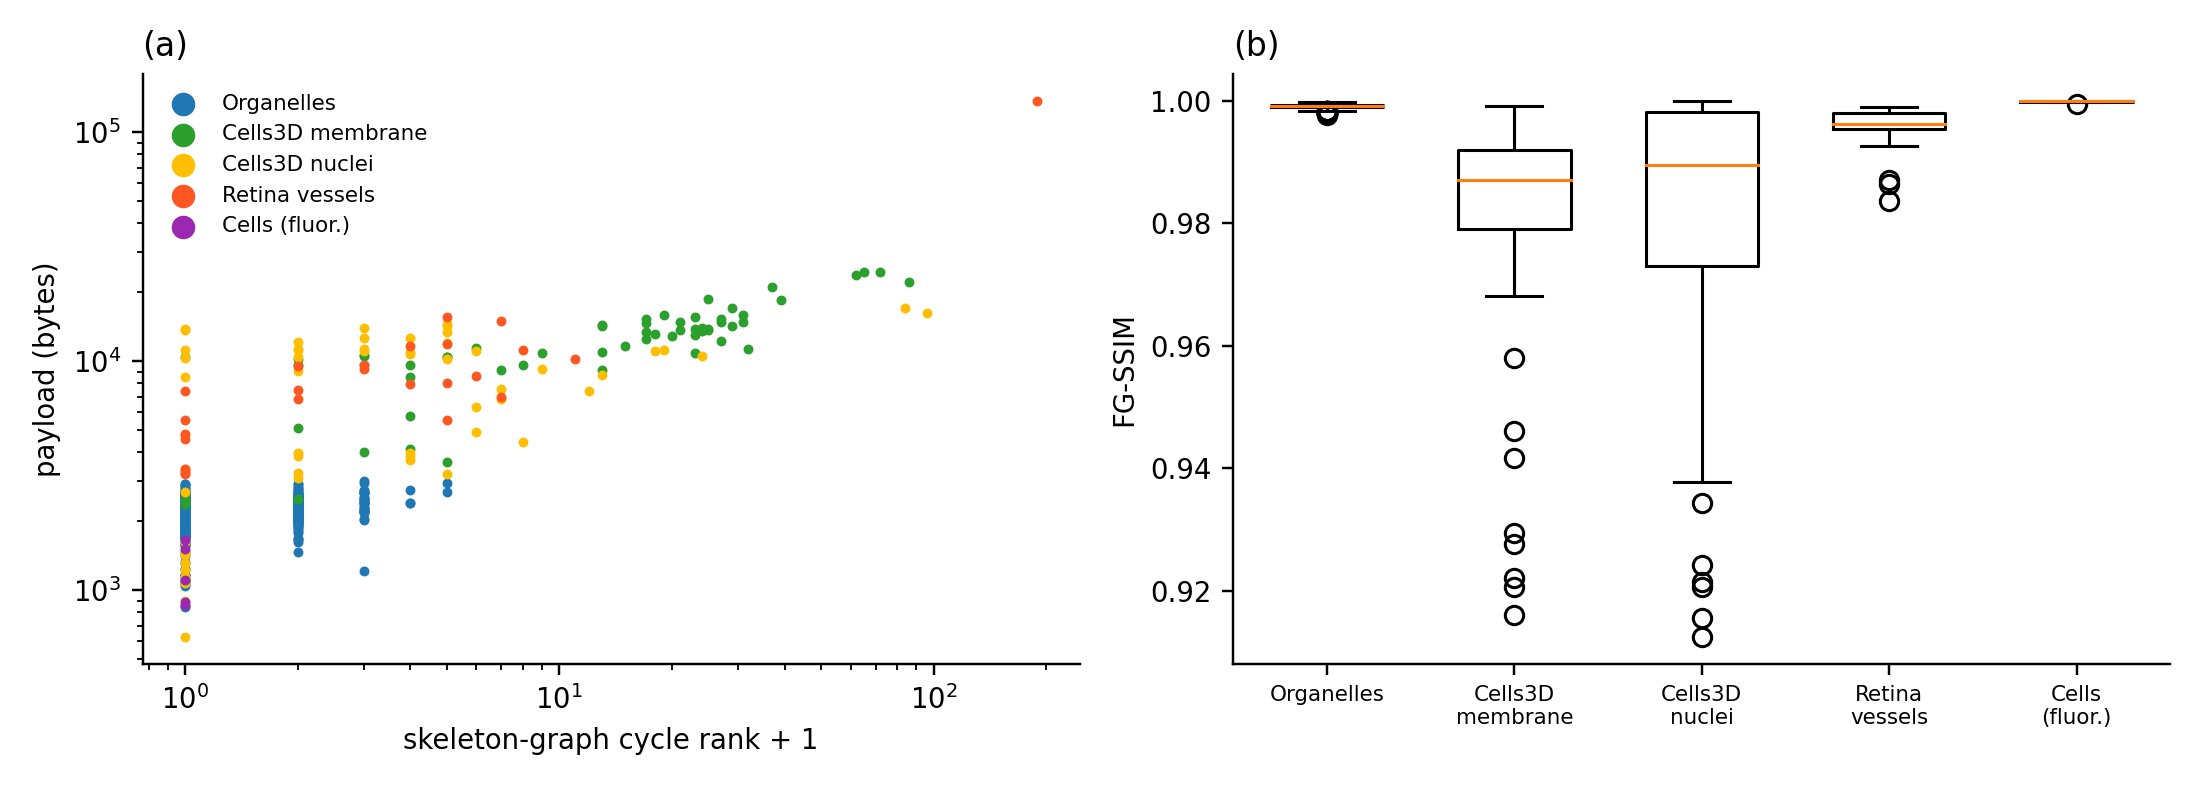
\includegraphics[width=\textwidth]{figures/fig_modality_scaling.png}
\caption{\textbf{Structure-proportional storage.} (a)~Payload against
skeleton-graph cycle rank across five modalities (log axes).
(b)~Foreground fidelity per modality.}
\label{fig:scaling}
\end{figure}

\begin{figure}[t]
\centering

\includegraphics[width=0.9\textwidth]{figures/cross_dataset_comparison.png}
\caption{\textbf{Cross-modality summary} (mean$\pm$s.d.): foreground and
full-image fidelity, payload, graph components and cycle rank for all five
modalities with the same encoder and configuration.}
\label{fig:cross}
\end{figure}

\subsection{A learned front end removes the segmentation bottleneck}
\label{sec:seg}
The foreground mask sets how faithfully $G$ describes the specimen. The
classical cascade finds the structure reliably but over-dilates it (recall
$\CSegRecm$, precision $\CSegPrecm$; Fig.~\ref{fig:segbottleneck}a).
The decoder partly compensates: because node widths drive the PSF shape,
the reconstruction's GT-IoU exceeds the mask's Seg-IoU on most images
(Fig.~\ref{fig:segbottleneck}b). A compact U-Net trained with a clDice
centreline loss~\cite{cldice} removes the bottleneck. As a standalone
segmenter it raises IoU on a seed-fixed validation split from 0.381 to
0.875, with precision and recall both near 0.93 (Table~\ref{tab:seg}).
Inside the pipeline it is added as a candidate that competes with the
classical segmenters under a plausibility gate, and with it the default
configuration reaches Seg-IoU $\DSegIoU$; forcing the learned mask on every
image gives $\LSegIoU$, and $\LHeldSegIoU$ on the $\LHeldN$ images the
network was not trained on, matching the standalone figure
(Fig.~\ref{fig:segbottleneck}c).

\begin{figure}[t]
\centering
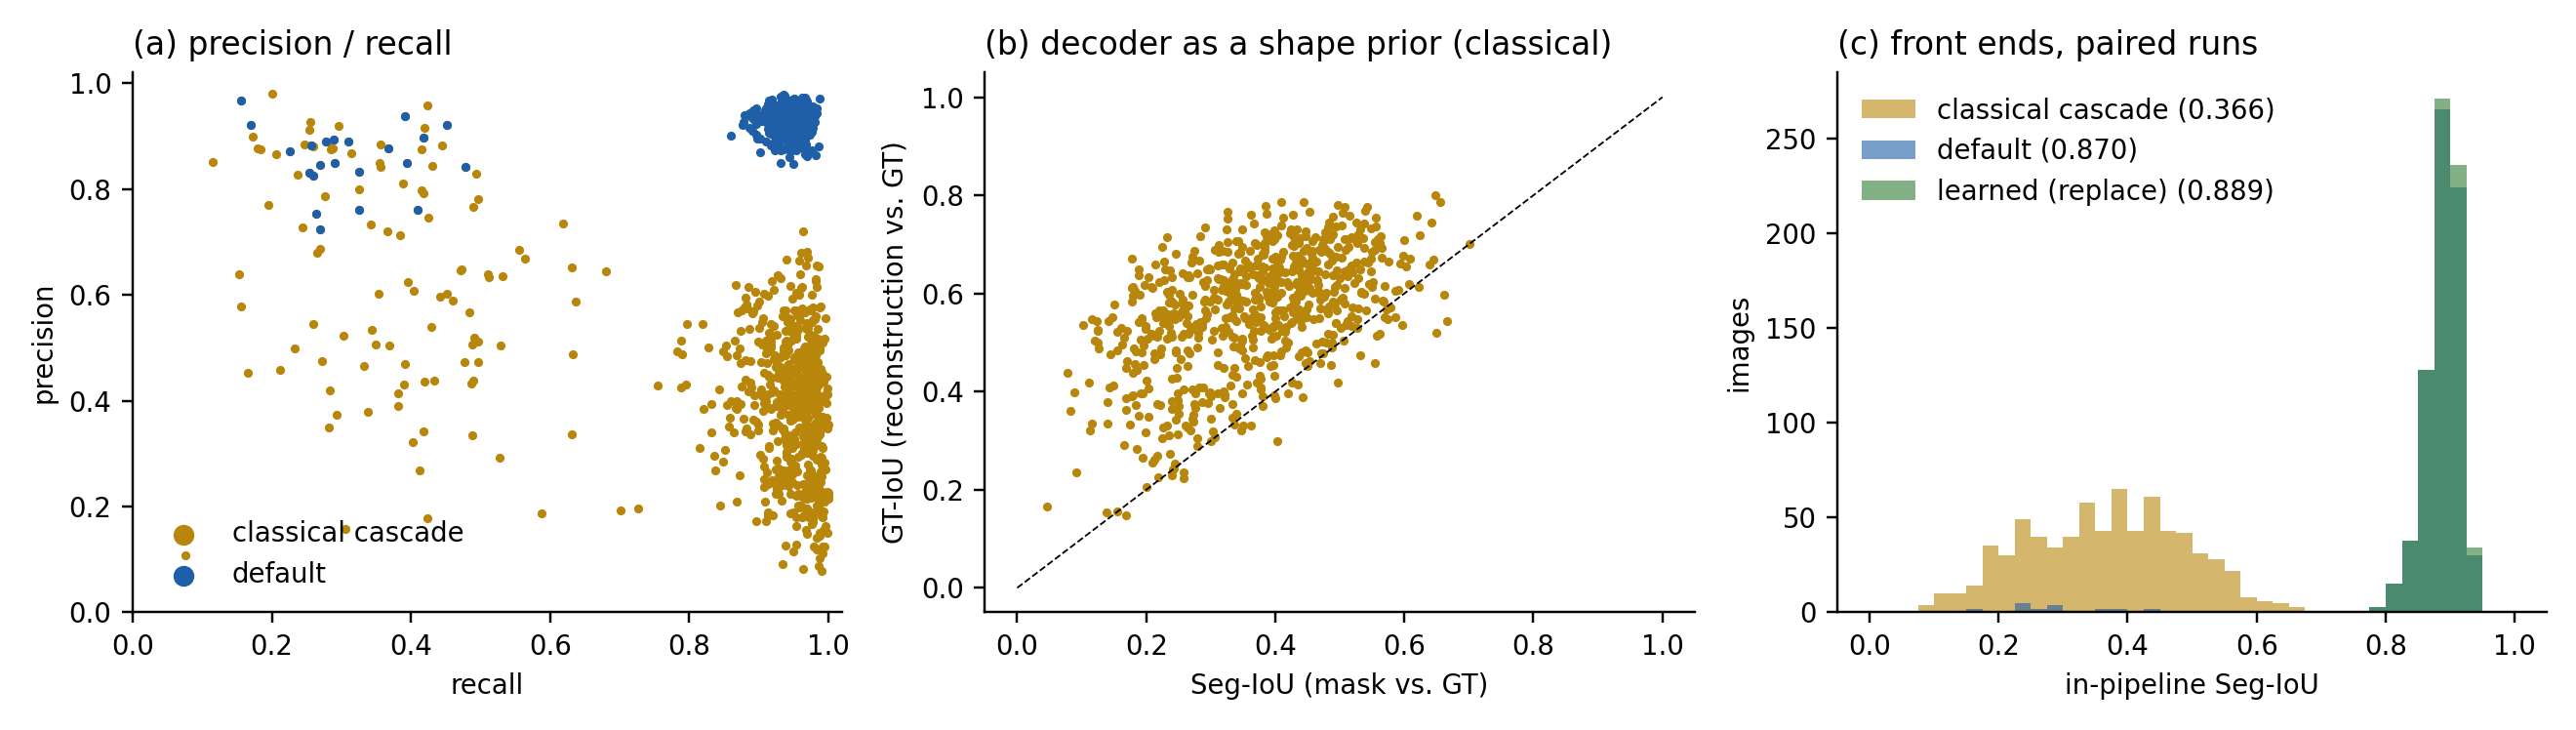
\includegraphics[width=\textwidth]{figures/fig_seg_bottleneck.png}
\caption{\textbf{Segmentation front ends on the organelle set.} (a)~The
classical cascade saturates recall at roughly half precision; the default
learned front end sits near the top-right corner. (b)~With the classical
cascade the decoder acts as a shape prior: GT-IoU exceeds Seg-IoU on most
images. (c)~In-pipeline Seg-IoU for the classical cascade, the default
configuration and the learned mask forced on every image, from paired runs
over the same 726 images.}
\label{fig:segbottleneck}
\end{figure}

\begin{table}[t]
\centering
\caption{\textbf{Standalone segmentation on organelles} (seed-fixed
validation split).}
\label{tab:seg}
\setlength{\tabcolsep}{7pt}
\begin{tabular}{lcccc}
\toprule
Front end & IoU & Precision & Recall & F1\\
\midrule
Classical cascade      & 0.381 & 0.440 & 0.850 & 0.540\\
clDice U-Net (learned) & \textbf{0.875} & 0.933 & 0.931 & 0.929\\
\bottomrule
\end{tabular}
\end{table}

\subsection{Polarity-agnostic retraining carries the representation to new modalities}
\label{sec:retrain}

A network trained only on bright-on-dark organelles transfers poorly to other
curvilinear modalities. On four external datasets---STARE and DRIVE retinal
vessels~\cite{stare,drive}, EPFL/Lucchi EM mitochondria~\cite{lucchi}, and IRM
microtubules---the whole pipeline collapses (Table~\ref{tab:retrain}, "old'').
We trace this to three compounding causes: (i)~\emph{polarity}---external
structures are dark-on-bright, the opposite of fluorescent organelles, so
vesselness filters and the organelle network respond to background;
(ii)~the organelle-calibrated quality score cannot \emph{rank} candidate
masks on these modalities; and (iii)~EM mitochondria are filled objects in
dense neuropil, not separable by any threshold or ridge filter (an oracle
dark-ridge Frangi reaches only 0.076 IoU).
Fig.~\ref{fig:oodfail} traces this collapse through the whole pipeline on an
EPFL EM slice and shows why the failure is total rather than graceful: the
segmentation stage floods 28\% of the frame, so skeletonisation returns the
medial axis of the \emph{background} lattice between organelles, the graph
inflates to 8676 nodes across 53 components, and the decoder faithfully
reconstructs that structure. Every downstream stage behaves
correctly given its input; the representation is only as meaningful as the
mask it is built from.

\begin{figure}[t]
\centering
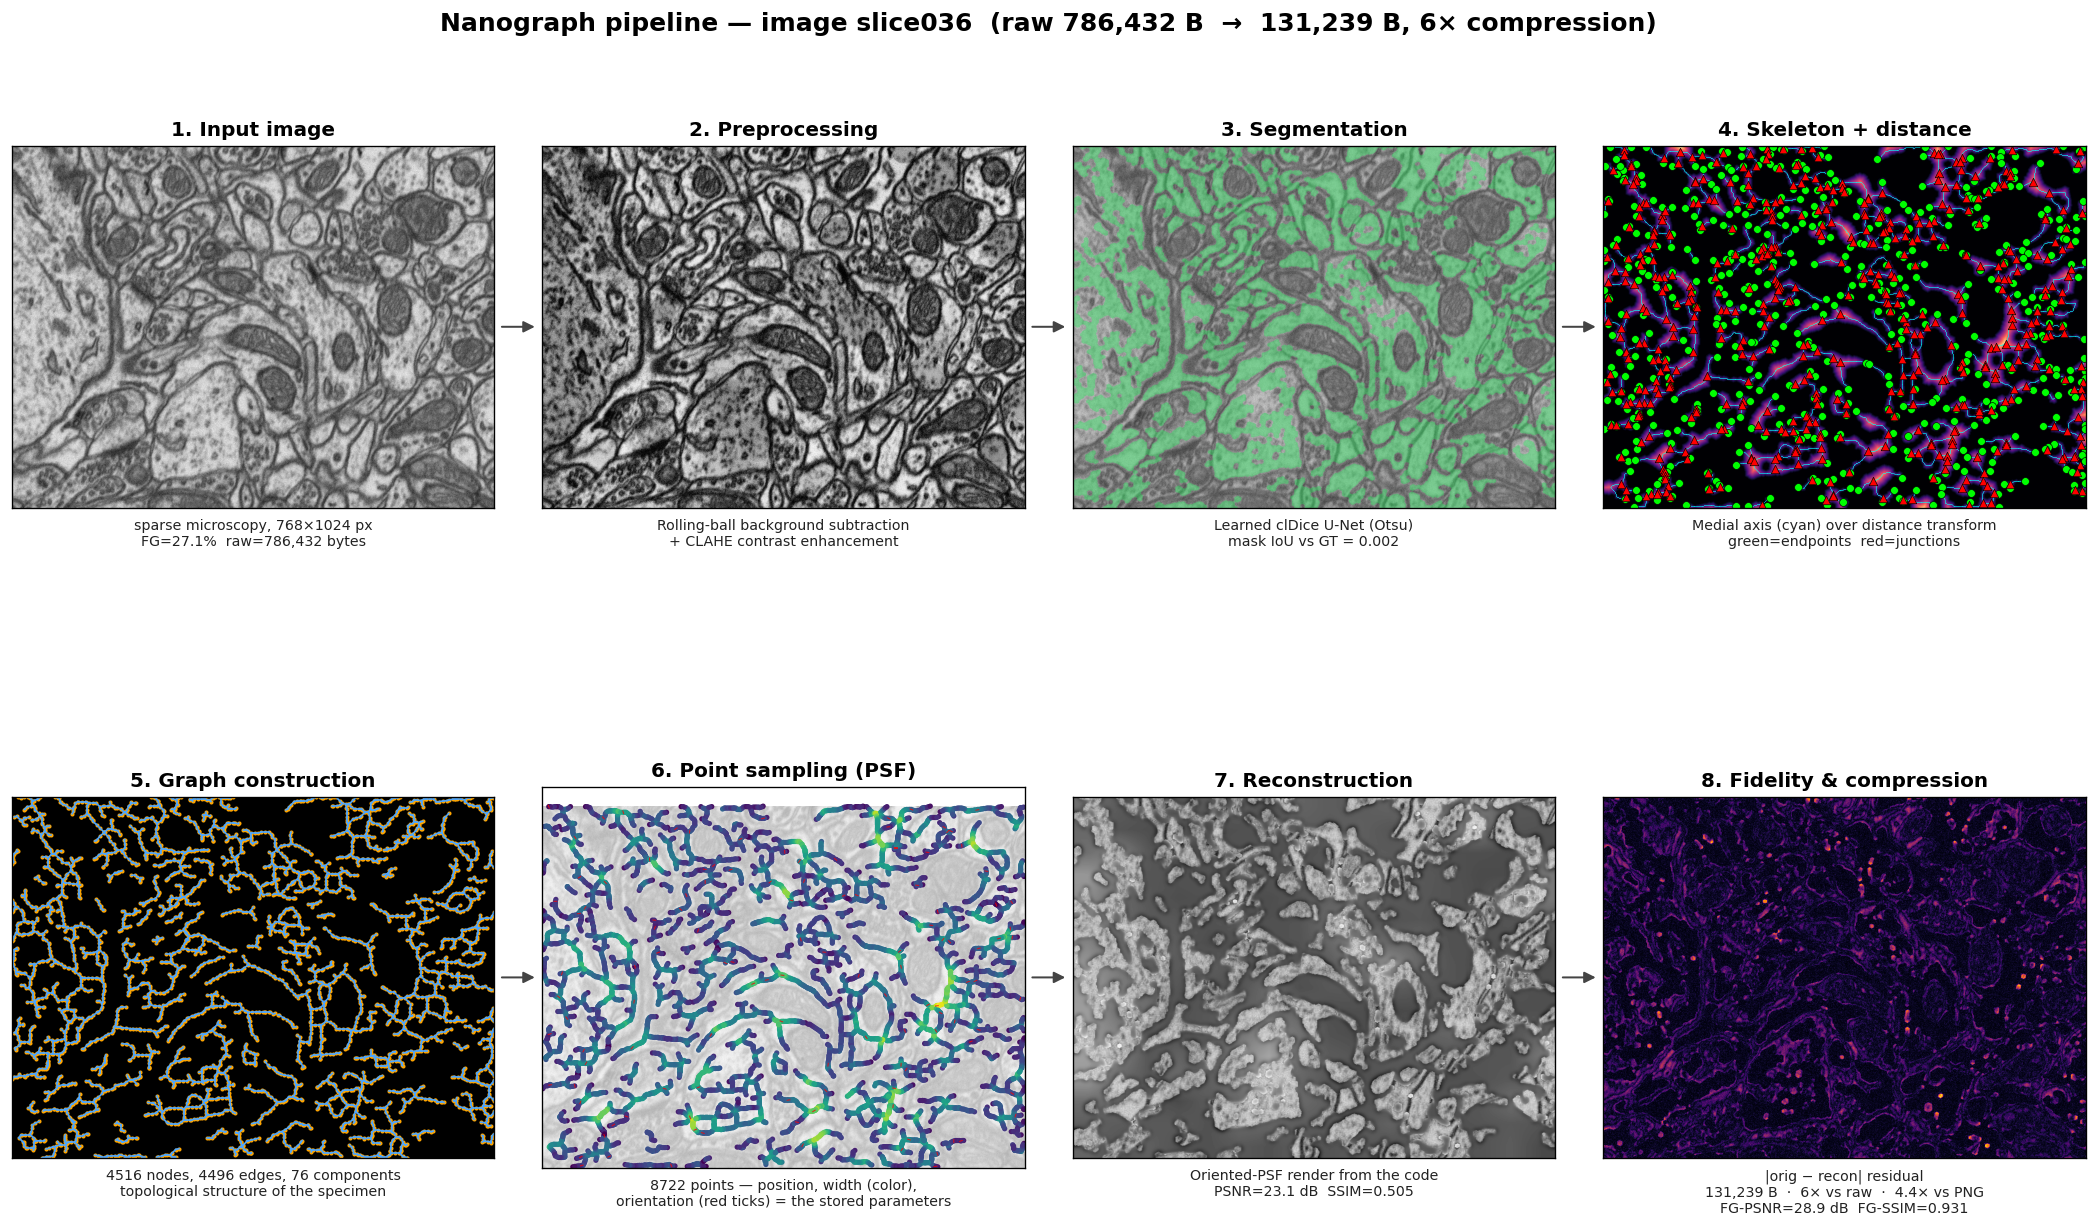
\includegraphics[width=\textwidth]{figures/fig_ood_failure.png}
\caption{Out-of-domain collapse on a held-out EPFL/Lucchi EM
mitochondria slice, using the organelle-domain front end. Stage~3
segments 28.1\% of the frame at 0.000 IoU against ground truth; stage~4
consequently skeletonises the background lattice rather than the
organelles; stage~5 yields an 8676-node, 53-component graph of that
lattice; and stages~6--8 reconstruct it faithfully. The pipeline does not
fail loudly---it produces a well-formed graph of the wrong structure,
which is precisely why the segmentation front end warrants the treatment
in this work.}
\label{fig:oodfail}
\end{figure}

We retrain a single clDice U-Net on the four datasets jointly with a
random-inversion augmentation that presents every structure in both
polarities, so the network needs no inference-time polarity detector.
Splits are leakage-free: independent images for vessels and filaments, and a
contiguous slice block with a guard gap for the EM volume. Validation IoU
rises to 0.64 (STARE), 0.56 (DRIVE) and 0.60 (microtubules), and to
\textbf{0.82} on EM mitochondria, from 0.001 (Table~\ref{tab:retrain},
Figs.~\ref{fig:drive}--\ref{fig:epfl}). The weights enter the pipeline as a
\texttt{for\_curvilinear} preset that uses the learned mask directly. The
network is genuinely polarity-agnostic: feeding images as-is matches an
oracle that picks the better polarity per image using ground truth
(Table~\ref{tab:polarity}).

\begin{table}[t]
\centering
\caption{\textbf{Segmentation IoU on four out-of-domain curvilinear
datasets}: classical/in-domain pipeline vs.\ the polarity-agnostic
multi-domain retraining (validation splits).}
\label{tab:retrain}
\setlength{\tabcolsep}{7pt}
\begin{tabular}{lcccc}
\toprule
 & STARE & DRIVE & Microtubules & EPFL mito (EM)\\
\midrule
Classical / in-domain & 0.056 & 0.100 & 0.021 & 0.001\\
Retrained             & \textbf{0.643} & \textbf{0.564} & \textbf{0.599} & \textbf{0.822}\\
\bottomrule
\end{tabular}
\end{table}

\begin{table}[t]
\centering
\caption{\textbf{Polarity-agnosticity.} IoU with images fed as-is vs.\ a
ground-truth oracle choosing the better of the two polarities per image.}
\label{tab:polarity}
\setlength{\tabcolsep}{7pt}
\begin{tabular}{lcccc}
\toprule
 & STARE & DRIVE & Microtubules & EPFL mito (EM)\\
\midrule
As-is             & \PolStareAsIs & \PolDriveAsIs & \PolMtAsIs & \PolEpflAsIs\\
Best-of-2 oracle  & \PolStareOracle & \PolDriveOracle & \PolMtOracle & \PolEpflOracle\\
\bottomrule
\end{tabular}
\end{table}

\begin{figure}[t]
\centering
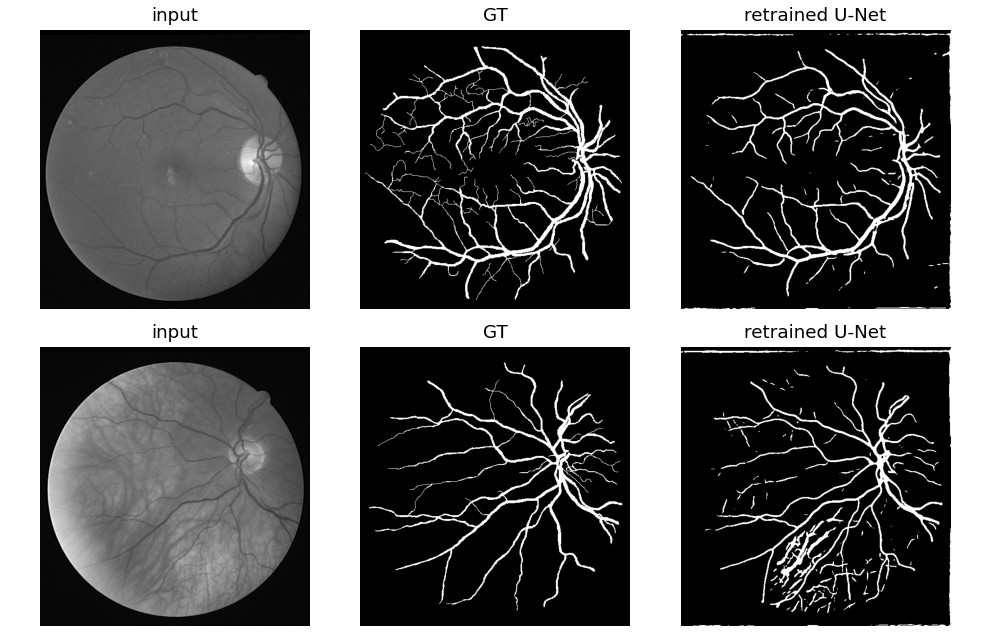
\includegraphics[width=0.8\textwidth]{figures/ext_drive.png}
\caption{\textbf{DRIVE retinal vessels}: input, ground truth and the
retrained segmentation used by the encoder, on two validation images.}
\label{fig:drive}
\end{figure}

\begin{figure}[t]
\centering
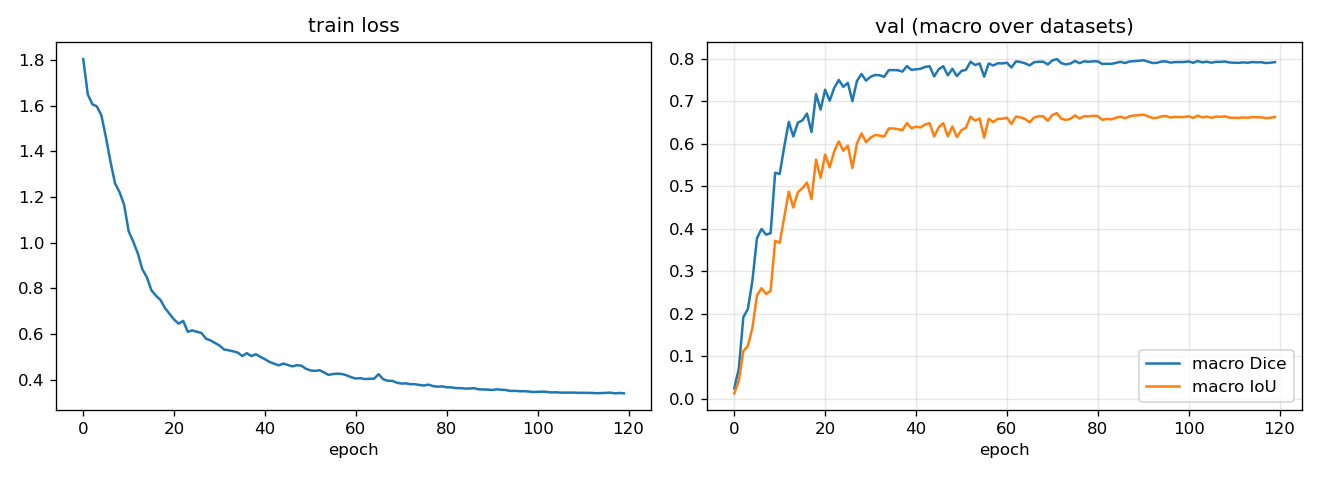
\includegraphics[width=0.62\textwidth]{figures/retrain_curves.png}
\caption{\textbf{Multi-domain retraining}: training loss and
macro-averaged validation Dice and IoU across the four datasets over 120
epochs.}
\label{fig:retraincurves}
\end{figure}

\begin{figure}[t]
\centering
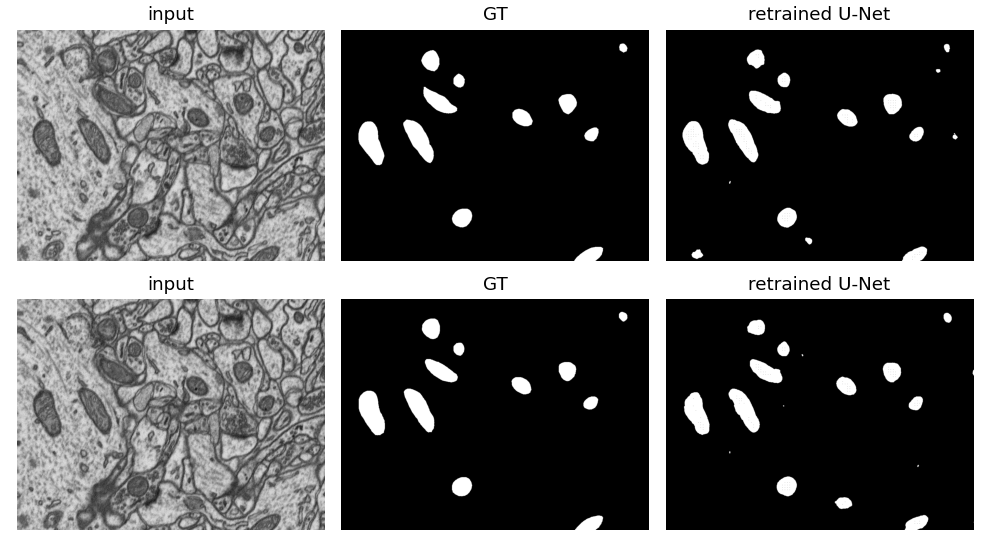
\includegraphics[width=0.8\textwidth]{figures/retrained_epfl.png}
\caption{\textbf{EPFL/Lucchi EM mitochondria}: input, ground truth and the
retrained segmentation on two slices from opposite ends of the guard-gapped
validation block.}
\label{fig:epfl}
\end{figure}

\subsection{The perturbation study maps how segmentation error reaches each stored invariant}
\label{sec:seg-perturb}
Graph-exactness guarantees that the stored invariants describe $G$; it says
nothing about how well $G$ describes the specimen when the mask is wrong. We
measure that dependence directly. For each of the 726 organelle images we
take the mask selected by the default configuration (mean Seg-IoU
$\PertBaseSegIoU$), degrade it in four controlled ways---morphological dilation and
erosion at radii 1--5\,px (over- and under-segmentation), random removal of
5--40\% of connected components (missed detections) and random flips within
a 1--3\,px boundary band (noisy edges)---and rebuild the structure layer from each
degraded mask with the pipeline's own construction ($\PertN$ rebuilt
graphs). We record the change in each invariant relative to the graph of
the unperturbed mask, indexed by the degraded mask's Seg-IoU against ground
truth (Fig.~\ref{fig:segperturb}). The unperturbed graphs have a median of
$\PertBaseComp$ components and $\PertBaseCyc$ cycles.

The four error types affect the invariants very differently, and a single
Seg-IoU threshold does not summarise them.
\emph{Over-segmentation} leaves the component count largely intact: after
1\,px of dilation $\beta_0$ changes on $\PertDilOneBz\%$ of images, and after 5\,px (Seg-IoU
$\PertDilFiveSeg$) on $\PertDilFiveBz\%$, through merging of neighbouring structures. Mean width,
however, is biased immediately and in proportion ($\PertDilOneW\%$ at 1\,px, $\PertDilFiveW\%$ at
5\,px), and the cycle rank shifts by a median of $\PertDilCycLo$--$\PertDilCycHi$ cycles.
\emph{Under-segmentation} is benign at 1\,px ($\beta_0$ changes on $\PertEroOneBz\%$ of
images) but fragments structures at 2\,px and beyond ($\beta_0$ changes on
$\PertEroBzLo$--$\PertEroBzHi\%$ of images) while width changes by $\PertEroWLo$ to $\PertEroWHi\%$.
\emph{Boundary noise} is the most damaging error for topology: a 1\,px band of
flipped pixels changes $\beta_0$ on $\PertNoiseOneBz\%$ of images and adds a median of $\PertNoiseOneCyc$
spurious cycles, rising to $\PertNoiseThreeCyc$ at 3\,px, while width changes by about $\PertNoiseW\%$.
\emph{Missed detections} behave locally: removing components changes $\beta_0$
by construction but moves mean width by at most $\PertDropW\%$ and the cycle rank of the
remaining structures by at most a median of $\PertDropCyc$, i.e.\ losing a structure removes
its subgraph without corrupting the invariants of the structures that
remain.

Two practical consequences follow. First, the error mode matters more than
the IoU. The classical cascade's characteristic error is over-segmentation
(precision $\approx0.5$ at recall $\approx0.98$); under that error the stored
component count survives, but stored widths are biased upward and cycle
counts drift, which is why moving to the learned front end matters for
morphometry even where it barely changes $\beta_0$. Second, the cycle rank
should be compared only between graphs built from masks of the same
provenance: any process that roughens mask boundaries inflates it by orders
of magnitude.

\begin{figure}[t]
\centering
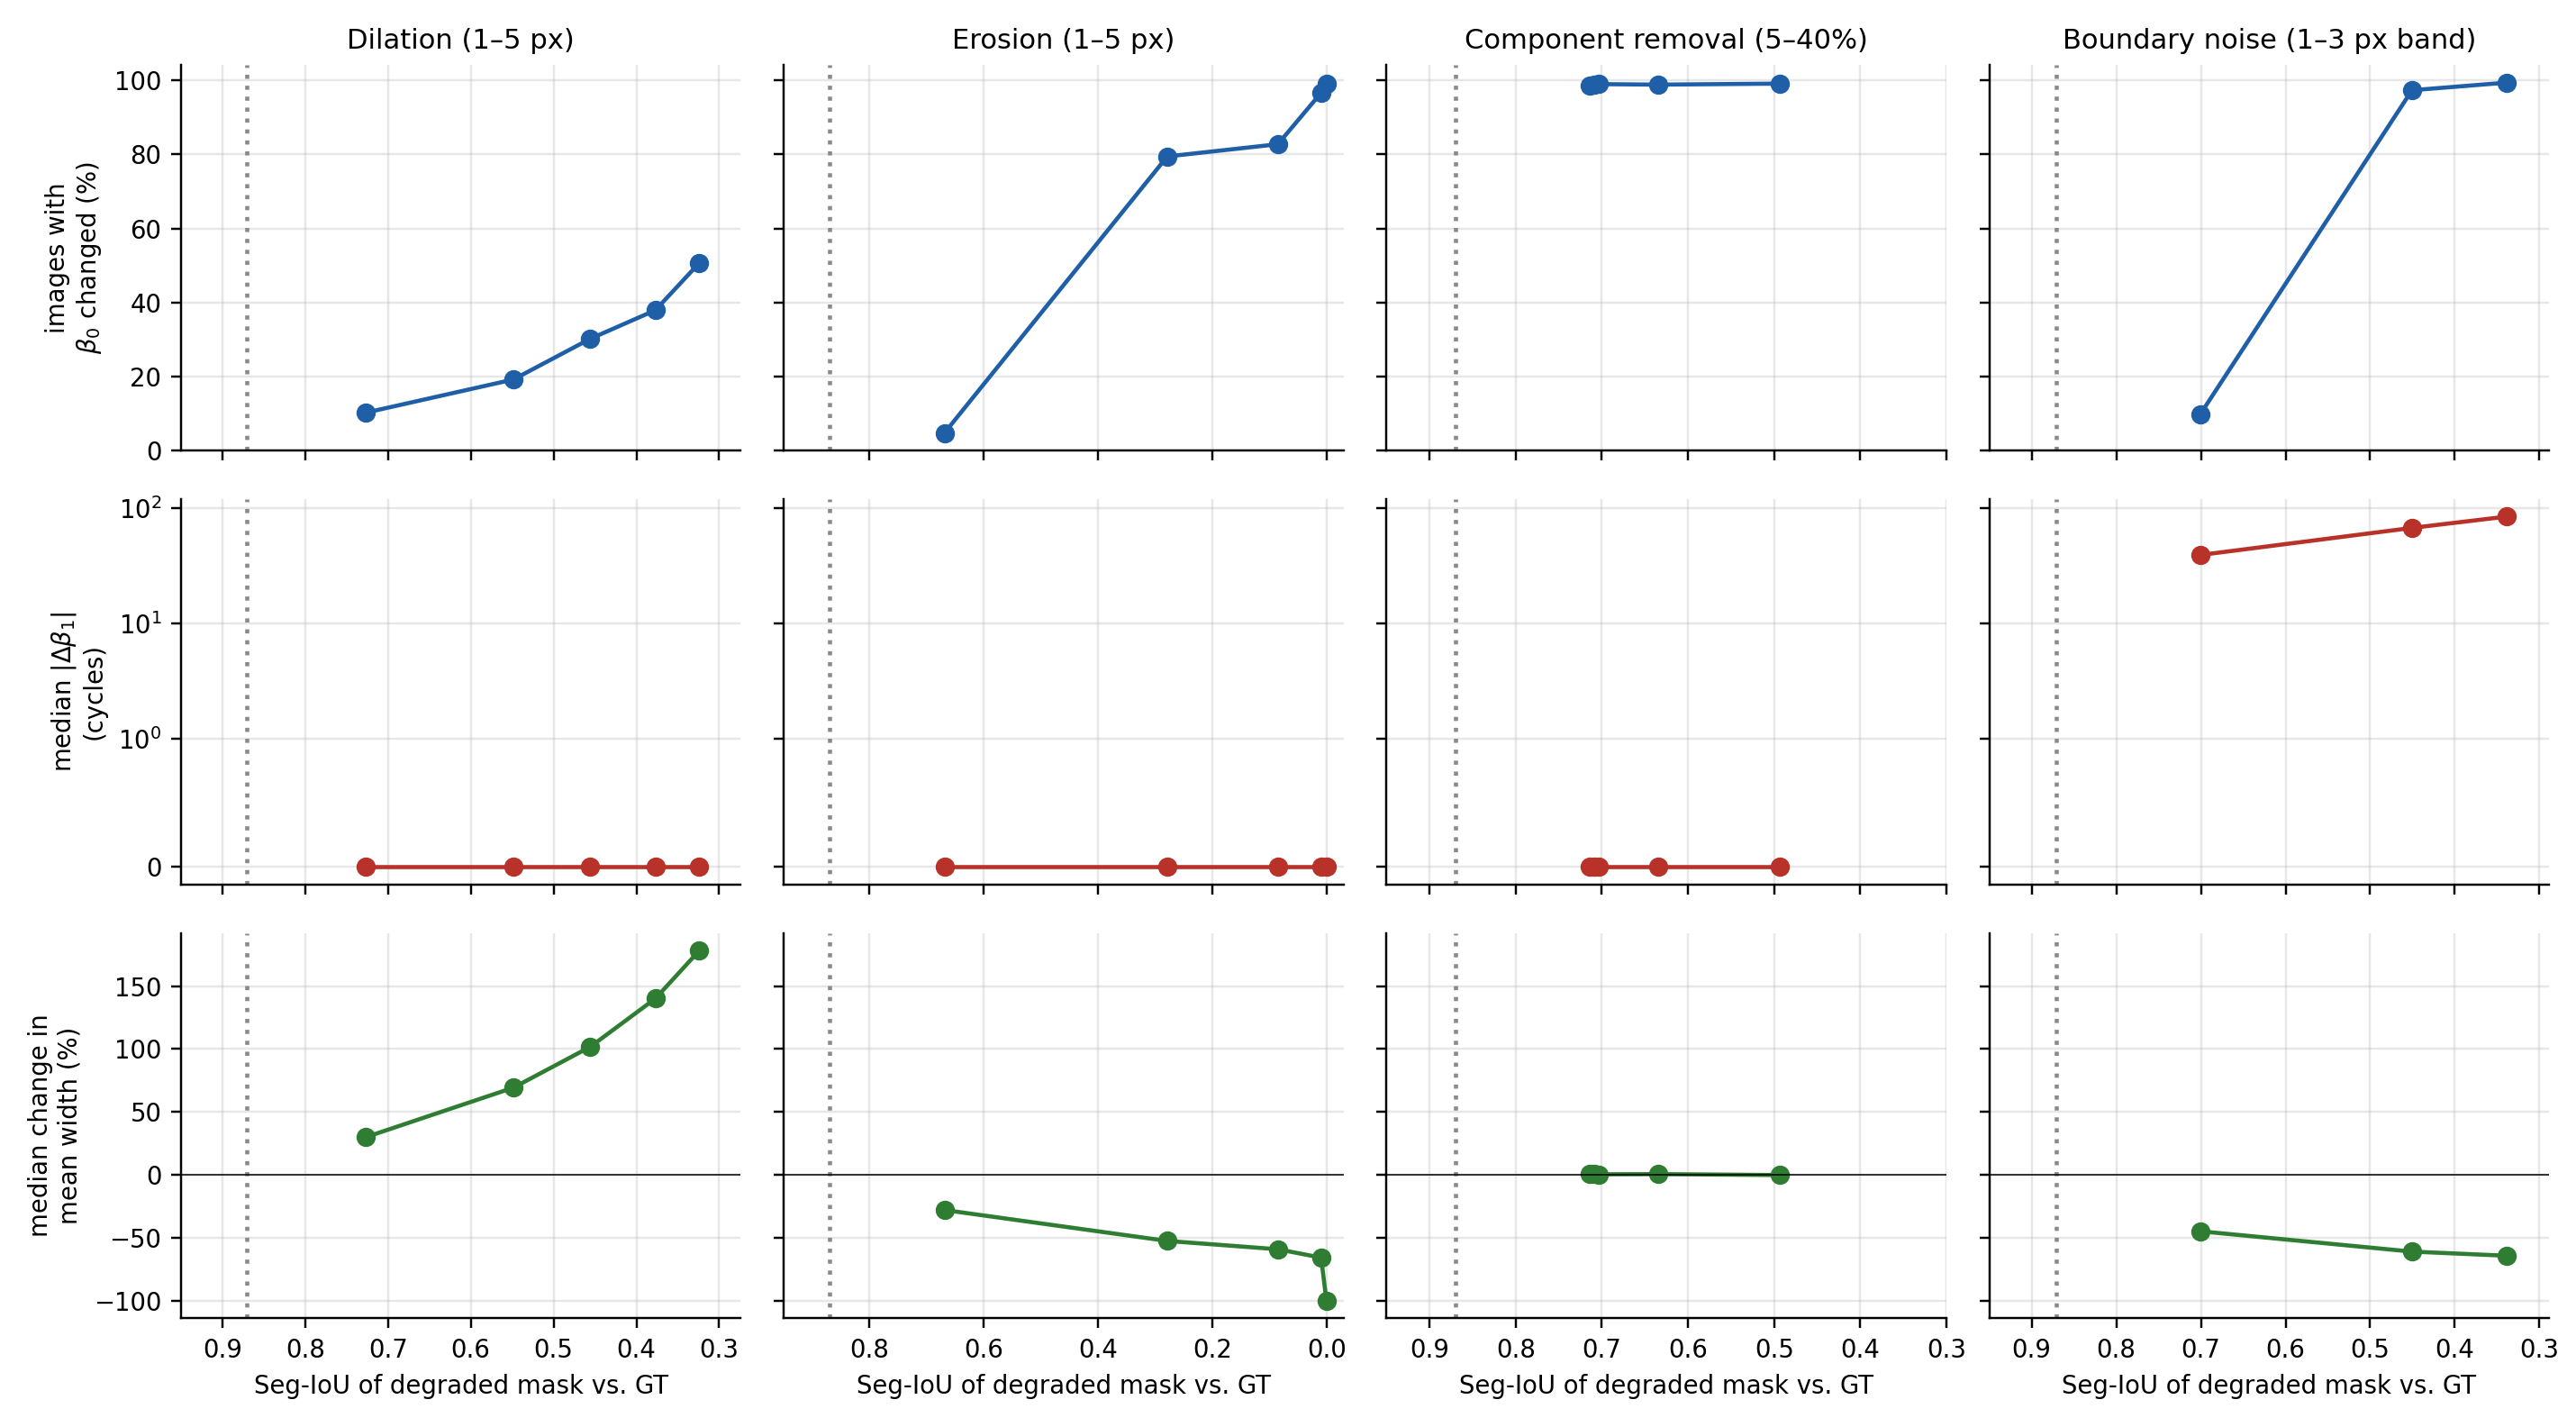
\includegraphics[width=\textwidth]{figures/fig_seg_perturb.png}
\caption{Propagation of segmentation error into the stored invariants on the
726-image organelle set. Each column degrades the mask selected by
the default configuration in one controlled way; the x-axis is the degraded
mask's Seg-IoU against ground truth (reversed), and the dotted line marks
the unperturbed operating point ($\PertBaseSegIoU$). Rows: fraction of images whose
component count $\beta_0$ changes; median absolute change in cycle rank
$\beta_1$ (symlog); median relative change in mean width. Over-segmentation
preserves $\beta_0$ but biases width; boundary noise inflates the cycle
rank by hundreds; component removal changes $\beta_0$ by construction while
leaving the other invariants intact.}
\label{fig:segperturb}
\end{figure}

\subsection{The representation transfers to further mitochondrial acquisitions}
\label{sec:mito-gen}
We applied the default pipeline, unchanged, to three further mitochondrial
sources (Table~\ref{tab:mitogen}, Fig.~\ref{fig:mitogen}; Methods). On the
73-frame simulated temporal clip (four unbranched mitochondria in elastic
motion, from a separate dynamic simulator~\cite{cods}), segmentation holds
up across frames (Seg-IoU $\ClipSegIoUm$, GT-IoU $\ClipGTIoUm$; with the
learned mask forced, Seg-IoU $\ClipLSegIoUm$). This is simulated evidence;
its ground truth is used against the stored graph in
Section~\ref{sec:truth}. On an independent live-cell STED
dataset~\cite{balakrishnan2024sted}, the organelle network, applied
zero-shot, produces clean masks and graphs where the classical cascade is
confounded by background haze; the outer-membrane label makes each tubule
appear as two parallel walls, which the graph traces as paired filaments
(about $\StedNodesm$ nodes and $\StedBytesm$\,kB per $600\times600$ frame).
On an independent confocal dataset with per-slice expert
masks~\cite{zhanghao2023mito}, the simulation-trained front end agrees
poorly with the annotation (Seg-IoU $\MitoSegIoUm$, precision $\MitoPrec$ at
recall $\MitoRec$): much of the predicted foreground lies outside the
annotated structures. This dataset is one of the four used to train the
real-data front end in Section~\ref{sec:real}.

\begin{table}[t]
\centering
\caption{\textbf{Further mitochondrial acquisitions} (mean$\pm$s.d.).
Temporal clip: 73 correlated frames of one simulated field of view. STED: no segmentation annotation is available. MITO:
$256\times256$ tiles of per-slice max-intensity projections.}
\label{tab:mitogen}
\footnotesize
\setlength{\tabcolsep}{4pt}
\begin{adjustbox}{max width=\linewidth}
\begin{tabular}{lcccc}
\toprule
 & $n$ & Seg-IoU & FG-PSNR (dB) & Bytes\\
\midrule
\tabinput{tables/tab_mitogen_body.tex}
\bottomrule
\end{tabular}
\end{adjustbox}
\end{table}


\subsection{Where pixel codecs are the better tool}
\label{sec:codec}
For completeness we compared the full \method payload with JPEG, WebP and
JPEG~2000 at matched bytes, as image codecs (Table~\ref{tab:codec},
Fig.~\ref{fig:codec}; Methods). By that criterion the codecs win. Photometric fidelity inside the
simulator's ground-truth mask (GT-FG-PSNR $\DGTFGPSNRm$ vs.\
$\DJpegGTFGPSNRm$\,dB) and over the full image favours them, because they
spend their bits on texture and background that \method deliberately
summarises. Foreground localisation from the regenerated image is at parity
with JPEG: GT-IoU is higher for \method on \DGTIoUWins{} images, with a
paired 95\% confidence interval of the mean difference of $\DGTIoUWinsCI$.
It follows segmentation quality: with the classical cascade, JPEG is ahead
(\method higher on \CGTIoUWins{} images). Pixel codecs are the right choice
when the image itself is the product. The comparison that matters for
\method is the analysis comparison of Sections~\ref{sec:downstream}
and~\ref{sec:real}.

On the annotated out-of-domain datasets (Methods), the pipeline reproduces
the retrained segmenter's accuracy inside the encoder (Seg-IoU
$\CgStareSegIoUm$/$\CgDriveSegIoUm$/$\CgEpflSegIoUm$/$\CgMtSegIoUm$ on
STARE/DRIVE/EM/microtubules). There, dense vasculature raises the
structure-proportional payload to about $\CgStareBytesm$\,kB per image, a
budget at which JPEG is near-transparent and leads on GT-FG-PSNR
($\CgStareJpegGTFGPSNRm$ vs.\ $\CgStareGTFGPSNRm$\,dB on STARE). Conversely, on
sparse filaments and EM the graph is often smaller than the smallest file
JPEG can produce at any quality (\CgMtNoJpeg{} microtubule and
\CgEpflNoJpeg{} EM images), a regime in which no byte-matched pixel codec
exists.

\begin{table}[t]
\centering
\caption{\textbf{Byte-matched codec comparison} on 726 organelle images,
default configuration (mean$\pm$s.d.). Codec quality is chosen by binary
search to match \method's payload; achieved bytes are reported because
JPEG~2000's rate control is coarse. Self-IoU wins compare each
reconstruction against \method's own mask.}
\label{tab:codec}
\footnotesize
\setlength{\tabcolsep}{4pt}
\begin{adjustbox}{max width=\linewidth}
\begin{tabular}{lccccc}
\toprule
 & Bytes & Full PSNR & Full SSIM & FG-PSNR & Self-IoU (\method wins)\\
\midrule
\method    & $\DBytes$ & $\DFullPSNR$ & $\DFullSSIM$ & $\DFGPSNR$ & --\\
JPEG       & $\DJpegBytes$ & $\DJpegFullPSNR$ & $\DJpegFullSSIM$ & $\DJpegFGPSNR$ & \DSelfIoUWinsJpeg{} ($\DSelfIoUWinsJpegPct\%$)\\
WebP       & $\DWebpBytes$ & $\DWebpFullPSNR$ & $\DWebpFullSSIM$ & $\DWebpFGPSNR$ & \DSelfIoUWinsWebp{} ($\DSelfIoUWinsWebpPct\%$)\\
JPEG~2000  & $\DJtwoBytes$ & $\DJtwoFullPSNR$ & $\DJtwoFullSSIM$ & $\DJtwoFGPSNR$ & \DSelfIoUWinsJtwo{} ($\DSelfIoUWinsJtwoPct\%$)\\
\bottomrule
\end{tabular}
\end{adjustbox}
\end{table}


\begin{figure}[t]
\centering
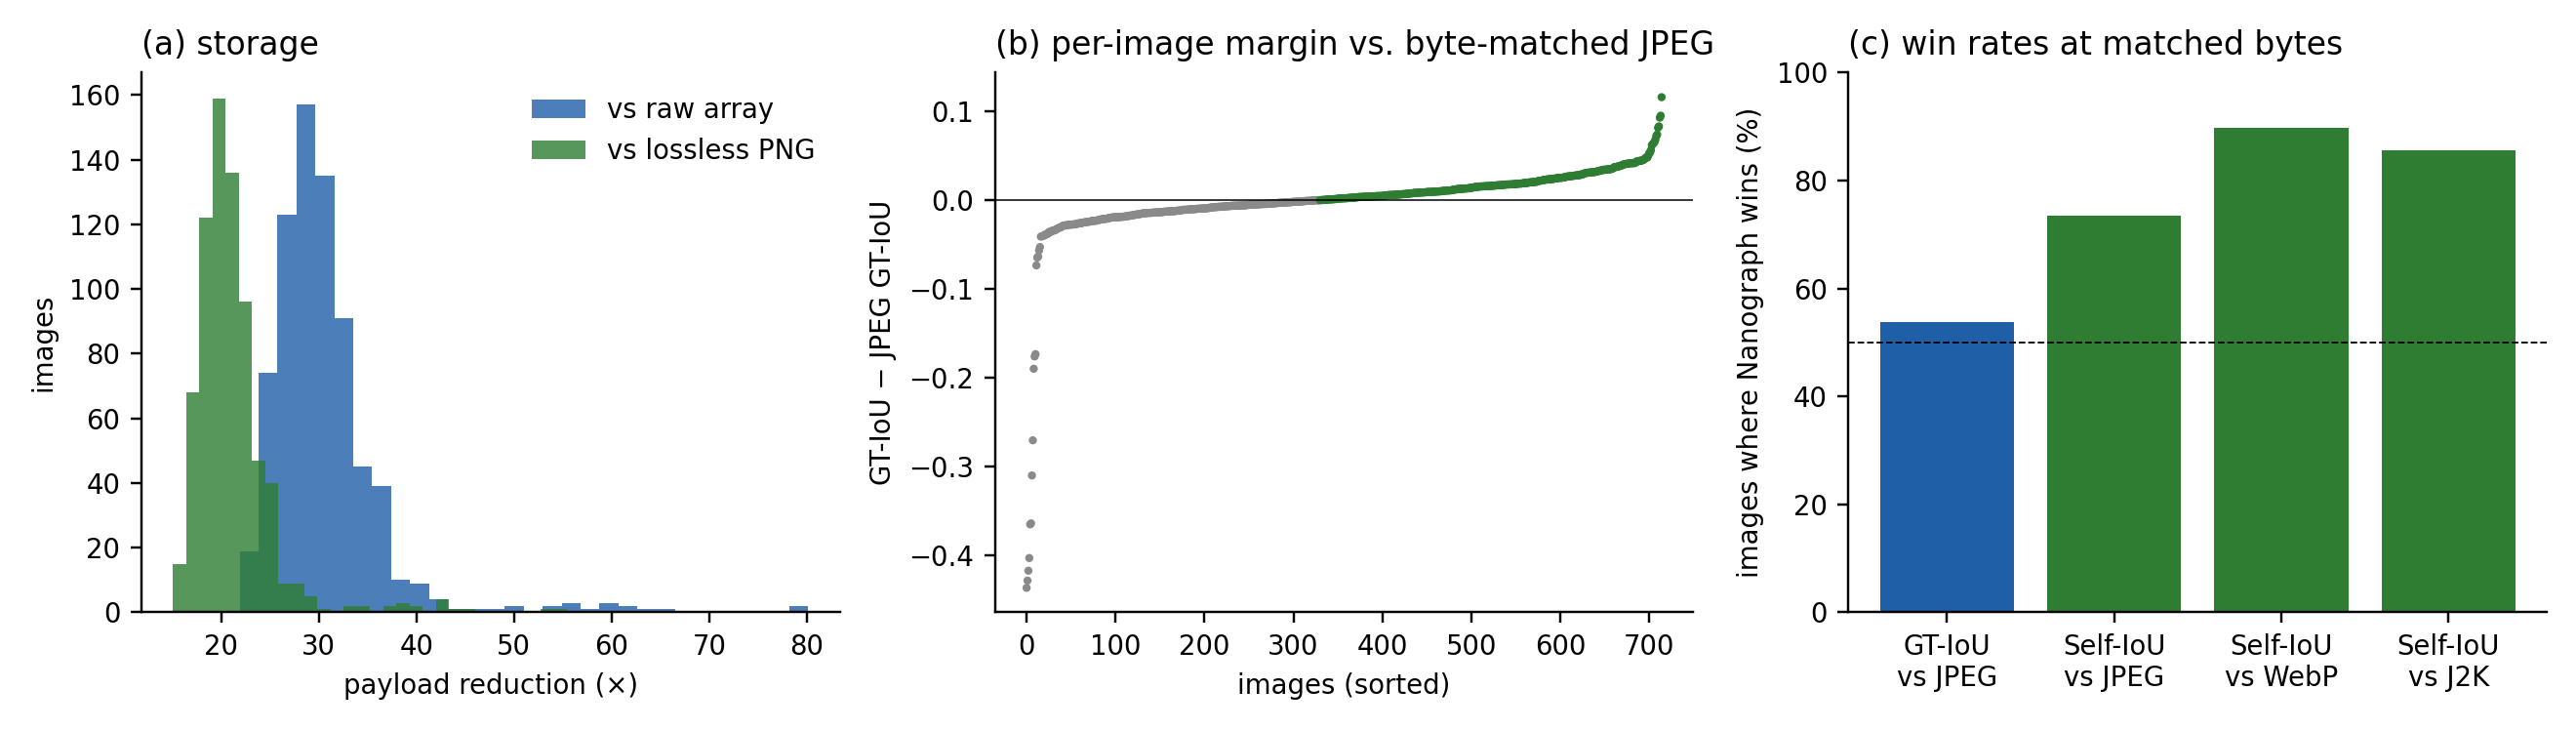
\includegraphics[width=\textwidth]{figures/fig_codec_rd.png}
\caption{\textbf{Compression behaviour on the organelle set.} (a)~Payload
reduction relative to the raw array and to lossless PNG. (b)~Per-image
GT-IoU margin over byte-matched JPEG (green: \method ahead). (c)~Win rates
at matched bytes against independent ground truth (blue) and against
\method's own mask (green).}
\label{fig:codec}
\end{figure}

% =====================================================================
\section{Discussion}
% =====================================================================
\method makes the geometry of a curvilinear image a stored, queryable
object. Its structure layer is the analysis of the segmentation it encodes,
costs about half the bytes of that segmentation stored losslessly, and is read
in about a millisecond. Against a pixel archive, analysis read from it
agrees better with the reference on simulated organelles, and on real
annotated mitochondria a JPEG must be several times larger to support the
same analysis. Against the true simulated geometry it is as informative as
the simulator's own mask. The appearance layer regenerates the image when
it is needed.

We do not claim that \method is a better image codec. When the image is
the product---for display, for photometric measurement, or for analyses
not yet defined---a pixel codec at the same budget reproduces it better,
and given the several kilobytes of the full payload, a JPEG is nearly
lossless and supports the same analysis as the original. The two formats
are built for different jobs. \method is for archives whose purpose is the
structure. There, storage, analysis and reconstruction become reads of one
object, and the analysis is done once, at encoding, with a declared
segmenter and a declared cleanup rule, rather than repeated inconsistently
by every user of the data.

The work also turns segmentation, the limitation named by every earlier
system in this line, into a studied and retrainable component: a
centreline-aware front end for simulated organelles, a front end trained on
four real mitochondrial datasets, a polarity-agnostic retraining that
carries the representation to vessels, filaments and EM, and a
perturbation map that tells users which stored invariants to trust under
which kind of mask error.

\subsection{Towards temporal tracking and event detection}
The representation established here is intended as the substrate for a further
question: whether morphological \emph{events} inside living cells can be
detected by monitoring how a structure's graph changes between timepoints,
rather than by tracking pixels. Because \method already exposes connectivity,
$\beta_0$/$\beta_1$ and per-branch morphometry as stored attributes, a
divergence between the graphs of the same structure at two instants is
directly computable on the representation---no re-segmentation, no
re-tracing. Realising this requires a correspondence between graphs across
time, which is where the module below begins.

An unevaluated but functionally complete temporal-tracking module
(\texttt{track.py}, $\sim$550 lines) already exists in the codebase, going
beyond the "scaffolded'' description we previously gave it. It replaces
per-frame skeletonisation---which is degenerate at sub-PSF self-contacts,
where a folded filament's two arms fuse into one blob and the medial axis
collapses to a single short line---with a single arc-length-parameterised 1D
curve per structure, seeded from the best-resolved frame (via graph-diameter
longest-path extraction~\cite{hagberg2008networkx}) and propagated frame-to-frame by optical-flow
advection~\cite{farneback2003} with an inextensibility-constrained snake
refinement, plus a "hybrid geodesic'' selector that falls back to the
propagated curve only when the single-frame skeleton geodesic looks
collapsed. The module is
implemented but unvalidated engineering, and is documented as such in the
released code; its systematic evaluation (ideally against
manually-tracked ground truth on a live-imaging time series) is deferred to
future work.

\subsection{Limitations}
The stored graph is exactly as good as the mask it is built from. Its
branch and junction under-counts relative to reference masks come from
segmentation, not storage, and each new acquisition type should contribute
training data: transfer between microscopes was limited in our
leave-one-dataset-out experiments. Near the optical limit, 2-D width is a
resolution-limited quantity; every 2-D route we evaluated overstates it,
including the simulator's own mask. The real test sets are small
(33--133 tiles), and tiles from one frame are correlated. The simulated
evaluation set was regenerated with the organelle simulator's settings; it
matches the original set closely but not exactly. The out-of-domain
datasets are small and their figures are validation estimates, and the EM
result comes from one volume with a guard-gap split. Payload grows with
structural complexity, so on dense vasculature the full payload reaches a
budget at which a pixel codec is near-transparent.

\subsection{Outlook}
Natural extensions are 3-D graphs; systematic validation of the temporal
module against ground-truth trajectories, for which mitochondrial network
tracking provides a protocol~\cite{wang2023mitotnt}; further real
acquisitions for the segmentation front end; and graph-native downstream
models that operate on the structure layer directly.

% =====================================================================
\section{Methods}\label{sec:method}
% =====================================================================
\begin{figure}[t]
\centering
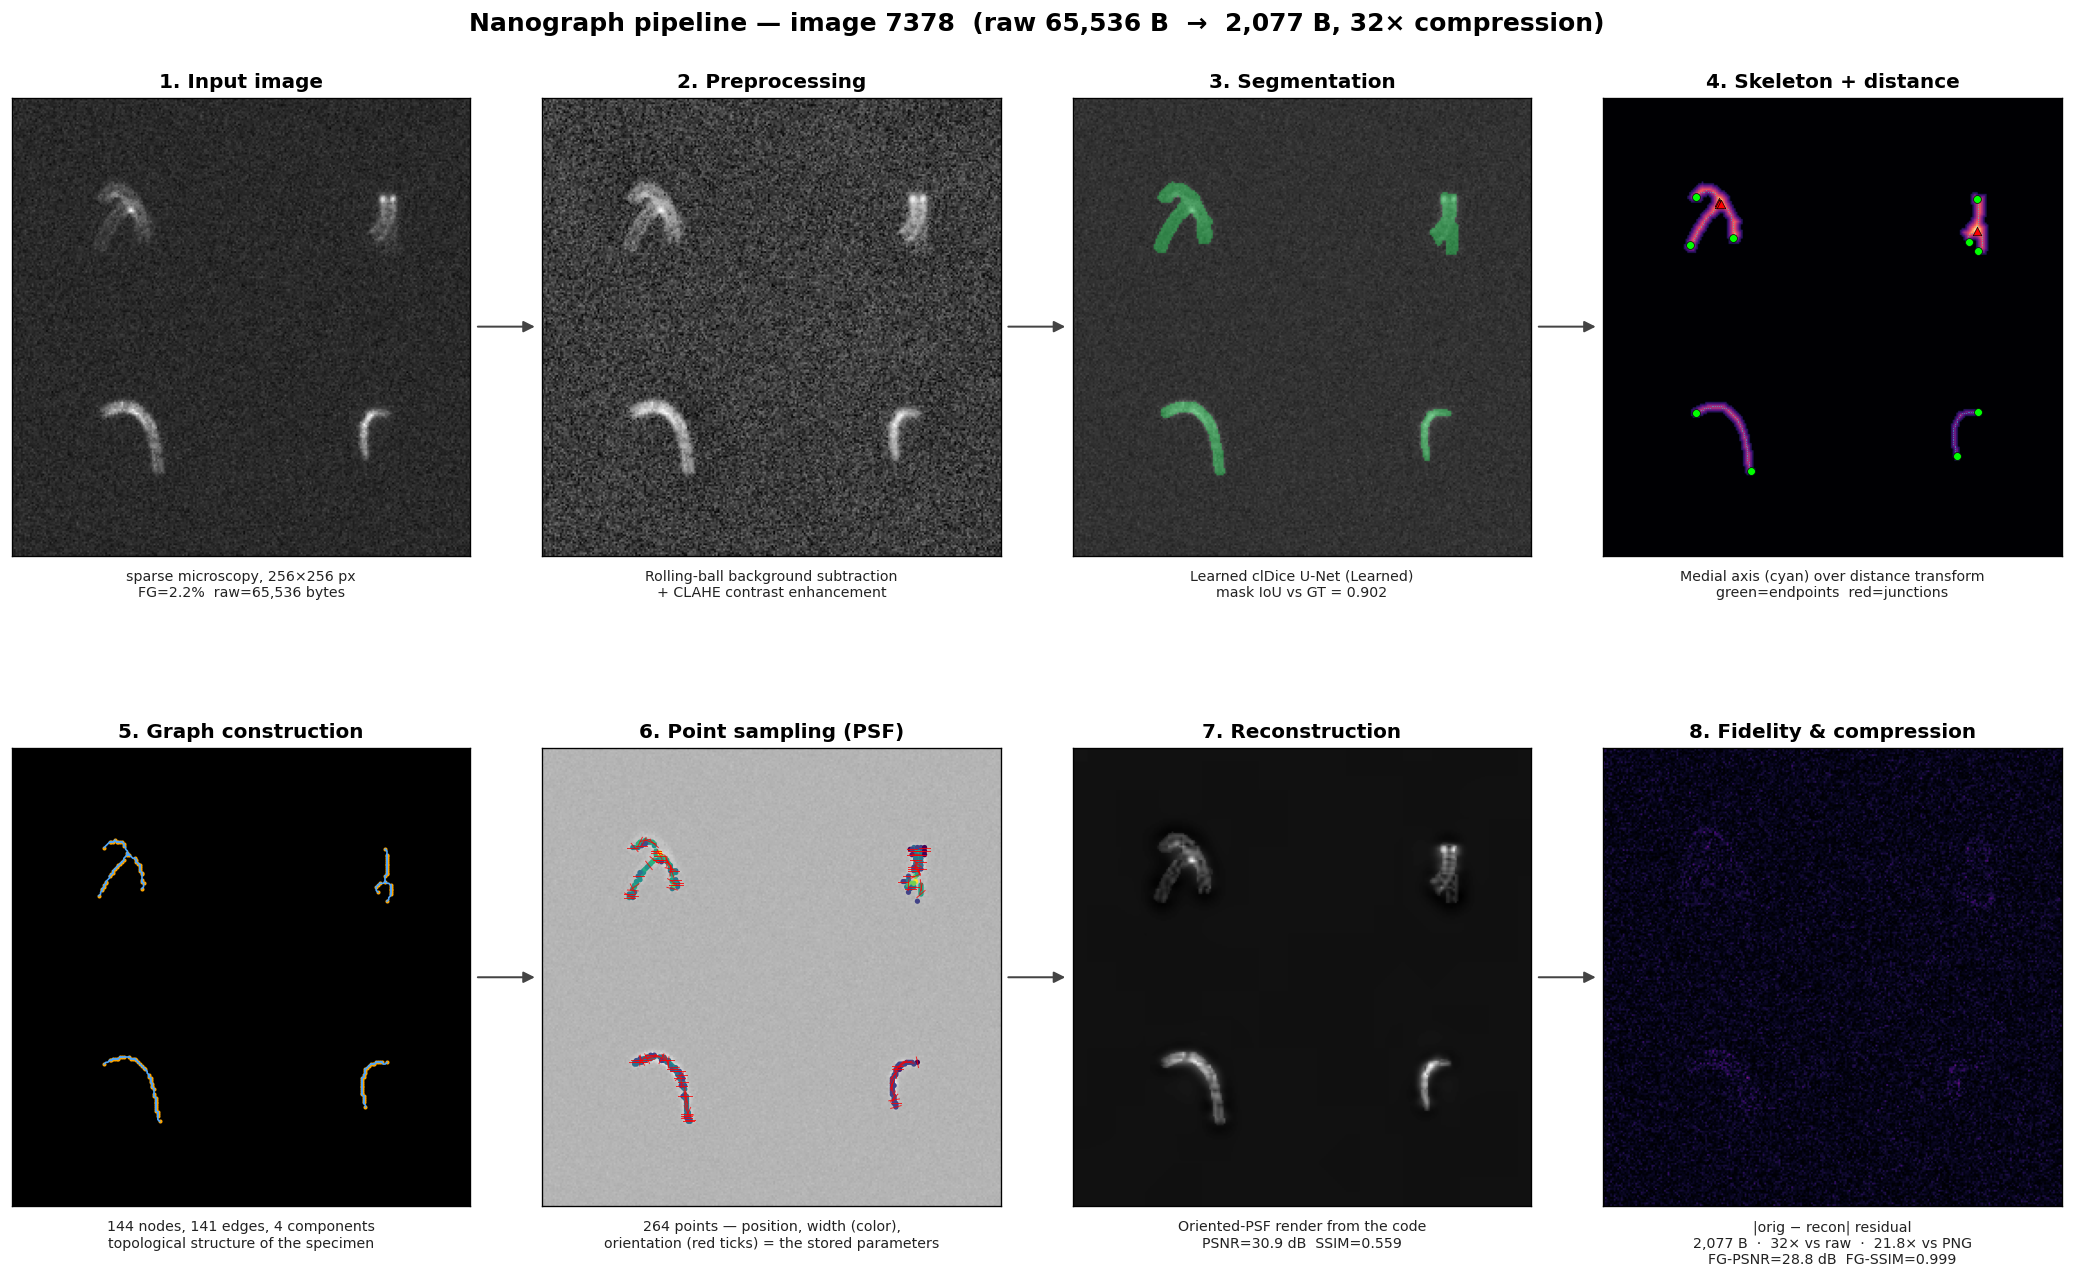
\includegraphics[width=\textwidth]{figures/pipeline_overview.png}
\caption{\textbf{The eight encode stages} on one organelle image:
input, preprocessing, foreground segmentation, skeleton with distance
transform, graph construction, oriented-PSF point sampling, reconstruction
and the reconstruction residual.}
\label{fig:stages}
\end{figure}

% =====================================================================
\subsection{Preprocessing and polarity normalisation}
The image is background-subtracted with a rolling-ball estimator~\cite{ballpark}
and locally contrast-normalised (CLAHE). Because curvilinear structures of
interest can appear either bright-on-dark (fluorescence organelles) or
dark-on-bright (brightfield/absorption imagery such as retinal fundus
photographs or EM), preprocessing first estimates image \emph{polarity} via a
morphological black-/white-top-hat ratio (structuring-element size 15\,px,
inversion threshold 1.3) and inverts the image when the structure of interest
is dark. This runs automatically (\texttt{polarity='auto'}) unless overridden.

\subsection{Cascading foreground segmentation}
Foreground is extracted by a cascade of cheap segmenters---Otsu thresholding
and the Frangi~\cite{frangi} and Meijering~\cite{meijering} vesselness
filters---each scored by a weighted combination of six terms (contrast 0.30,
foreground coverage 0.10, boundary coherence 0.15, skeleton quality 0.15,
edge sharpness 0.15, expected-shape match 0.15) with early exit. An optional Segment Anything~\cite{sam} fallback is
invoked only when the best cheap score falls below 0.65; it was not enabled
in the runs reported here. Because thresholding
tends to over-predict (high recall, low precision), we add a learned
candidate: a compact U-Net~\cite{unet} trained with a combined Dice+BCE and
clDice~\cite{cldice} centreline loss. The centreline term specifically
penalises breaks in thin structure that area-weighted Dice ignores. By
default the learned mask competes with the classical cascade
(\texttt{learned\_mode='candidate'}) under a \emph{plausibility gate} that
only lets it compete when its predicted foreground fraction falls within
$[0.25,1.75]\times$ the expected range for the image type---this blocks
empty or flooded masks a single-domain network can emit out-of-distribution,
but it also means the learned candidate
is not guaranteed to win even where it is more accurate. A dedicated
\texttt{for\_curvilinear()} preset instead sets
\texttt{learned\_mode='replace'}, bypassing the cascade entirely for
dark-on-bright curvilinear imagery (Table~\ref{tab:retrain}). A \texttt{for\_real\_mito()} preset
likewise uses, in \texttt{replace} mode, the network trained on real
mitochondria (Section~\ref{sec:real}).

\subsection{Skeletonisation and the structure layer}\label{sec:graph}
The selected foreground mask is skeletonised~\cite{lee} and its Euclidean
distance transform gives a per-pixel radius. The skeleton is decomposed into
branches with skan~\cite{skan}. Every connected cluster of junction pixels
becomes one junction vertex at the cluster's centroid, and every endpoint
becomes an end vertex. Each branch is stored as a polyline between its two
vertices, simplified with the Douglas--Peucker algorithm (tolerance
0.75\,px) and subdivided so that no chord exceeds 8\,px. A branch that joins
two junctions keeps at least one interior point, so that adjacent junctions
are never contracted into one. Each polyline point stores its position and
radius. Each branch also stores its path length, measured on the
full-resolution skeleton before simplification. Closed loops without a
vertex are stored as cycles on a single vertex. The resulting graph
$G=(V,E)$ exposes, without reprocessing pixels: connected components
($\beta_0$), cycle rank ($|E|-|V|+\beta_0$ on the branch graph), branch and
junction counts, junction degrees, branch lengths, total length, width
along every branch, spatial extent and induced subgraphs. Curvature can be
derived from the polylines. We call these properties \emph{graph-exact}.
The term is deliberately narrow: they are exact properties of $G$, not
guaranteed properties of the specimen. Any error in the foreground mask
propagates into $G$ and is then represented exactly, and the accuracy of the
representation with respect to the specimen remains bounded by the
segmentation, a bound we quantify in Fig.~\ref{fig:segperturb}.

The earlier builder, kept as an ablation (\texttt{graph.builder='pixel'}),
sampled nodes at fixed spacing along skeleton pixels, joined them greedily
and did not store path lengths. Junction clusters then produced spurious
short cycles. Its stored cycle rank matched the mask's enclosed holes on
16\% of organelle images, against $\GraphCycEqPct\%$ for the branch
builder.

\subsection{Appearance layer}
The appearance layer carries the points from which the image is rendered.
They are sampled along the skeleton at fixed spacing, after spur pruning
(5\,px), gap bridging of collinear endpoints (at most 12\,px apart, cosine
alignment $\geq0.6$ at both ends) and removal of components with fewer than
3 points; these steps affect the rendering only, not the structure layer.
Each point carries width, intensity and a tangent orientation estimated from
a smoothed structure tensor~\cite{bigun1987structuretensor}.

\subsection{Oriented-PSF reconstruction}
Filaments are anisotropic, so isotropic Gaussians waste energy perpendicular
to the structure. \method reconstructs by convolving each sampled node with an
\emph{elliptical} PSF whose major axis is aligned to the node orientation
(default aspect ratio 2.5) and whose scale follows the node width. Points are
grouped by (scale, orientation) bins for efficient FFT convolution. A
$16\times16$ bilinearly-upsampled background grid (256\,bytes) restores the
low-frequency field that a single mean value cannot, and an optional
$8\times8$-block DCT residual~\cite{ahmed1974dct} (quality 30, capped at 50\%
of the point-data budget) recovers fine foreground detail that node-level PSF
placement misses.

\subsection{Error-guided refinement}
\label{sec:optimizer}
After the skeleton points are placed, a refinement stage re-renders the
point set, forms a foreground-restricted error map, and adds rendering
points at high-residual locations (at most 30 per iteration, up to 20
iterations) until the foreground error plateaus. The added points belong to
the appearance layer only; the structure layer is unaffected.

\subsection{Serialisation}\label{sec:compression}
The payload is a one-byte version tag and the length of the structure layer,
followed by the two layers. The structure layer stores vertices sorted by
row as position deltas, their kinds (2 bits) and radii, then for every
branch its end vertices, its path length (quantised to 1/4\,px) and its
interior polyline points as position deltas with radii predicted from the
preceding point (radius quantised to 1/4\,px); all integers are variable-length
coded and the layer is zlib-compressed. The appearance layer stores quantised
point attributes---position (row-delta coded), width, intensity and a 1-byte
orientation (256 levels over $[0,\pi)$, quantisation error $<0.4^\circ$)---the
background field and the optional residual, with width and intensity coded
predictively from already-decoded neighbours, compressed with zlib at level
9. The structure layer can be read without decompressing the appearance
layer. Every fidelity figure in this paper is computed on the image
rendered from the decoded payload, and every descriptor attributed to
\method on the structure layer decoded from it.

\subsection{Configuration and image-type presets}
\label{sec:config}
Every stage above is controlled by one of 127 explicit parameters, organised
into nine dataclasses (preprocessing 12, segmentation 37, reconstruction 15,
refinement 10, compression 11, image-type detection 14,
classification 6, evaluation 8, graph construction 14). Presets adapt
this configuration to different imaging regimes without hand-tuning:
\texttt{for\_image\_type()} adjusts background-subtraction kernel size and
expected foreground-fraction bounds for sparse vs.\ dense structures;
\texttt{for\_curvilinear()} swaps in the polarity-agnostic
multi-domain segmenter in unconditional \texttt{replace} mode for dark-on-bright
vessel/EM/filament imagery; and \texttt{for\_real\_mito()} swaps in the
network trained on real mitochondria.

\subsection{Datasets}
The main evaluation set is 726 \emph{simulated} fluorescence images of
mitochondria generated with the physics-based simulator of Sekh et
al.~\cite{sekh2021} (Airyscan variant). Each $256\times256$ image is a
$2\times2$ mosaic of independent $128\times128$ simulations, each holding one
or two unbranched tubular mitochondria (spline centrelines, 20--300\,nm
diameter, 42\,nm pixels) rendered through a Gibson--Lanni point-spread
function with Poisson noise. Its foreground masks are the simulator's
ground truth (emitter positions on the pixel grid), not manual
annotations; because the simulated structures are unbranched, junctions
and cycles in these masks arise only where tubes overlap in projection.
The set is distinct from the real UiTMito data~\cite{sekh2021} used by our
earlier systems. Four
unannotated cross-modality sets are encoded unchanged: Cells3D membrane
($N{=}60$), Cells3D nuclei ($N{=}60$), retinal vessels ($N{=}25$) and
fluorescence cells ($N{=}5$). Four annotated out-of-domain curvilinear
datasets are used for retraining and ground-truth-referenced evaluation:
STARE~\cite{stare} and DRIVE~\cite{drive} retinal vessels, EPFL/Lucchi EM
mitochondria~\cite{lucchi} and IRM microtubules ($n=20/20/10/66$). Three
further mitochondrial sources test transfer within the nominal domain: a
simulated 73-frame temporal clip ($285\times285$) of four unbranched
mitochondria in elastic motion, from a separate dynamic simulator whose
per-frame ground-truth skeletons are available; a public
live-cell STED dataset (U2-OS, TOM20 label, 345
frames)~\cite{balakrishnan2024sted}; and a public confocal dataset with
per-slice expert masks~\cite{zhanghao2023mito}, evaluated as
$256\times256$ tiles of max-intensity projections ($n=228$).

\emph{Simulation with geometry.} For the truth evaluation we regenerated
organelle-like images with the same simulator, calling its own geometry and
point-spread-function code and keeping what the original pipeline discards:
each tube's centreline and diameter. Batch settings (lateral extent, number
of tubes per patch and noise range) were calibrated so that the regenerated
images match the organelle set in foreground fraction, structure size and
intensity statistics. The true skeleton is every centreline drawn
8-connected on the pixel grid, so crossings in projection become junctions
exactly as any 2-D analysis must see them; the true width is the tube's
diameter. The temporal clip's truth is its per-frame skeleton polylines and
the median surface-to-skeleton distance of each mitochondrion~\cite{cods}.

\emph{Real mitochondria.} Four expert-annotated datasets were tiled into
$256\times256$ tiles after a per-frame (0.5, 99.8) percentile contrast
stretch; tiles with less than 0.5\% foreground were dropped. Splits are by
frame or cell, never by tile. EP1-UiT-Rat: 32 epifluorescence frames
($1024\times1024$), shuffled into 24/4/4 training/validation/test frames
(277/44/45 tiles). CBMI~\cite{cbmi}: the provided splits (165/20/68 tiles).
MITO~\cite{zhanghao2023mito}: cell M1 for training (its last slices for
validation) and cell M2 for testing (143/33/133 tiles). EP-UiT-Human: four
epifluorescence frames ($1024\times1024$; 33 tiles; annotation maps
thresholded at 128), used only for testing.

\subsection{Metrics}\label{sec:metrics}
\emph{Seg-IoU} is the IoU between the pipeline's selected foreground mask
and the reference mask (the simulator's ground truth on the simulated sets,
the expert annotation elsewhere). \emph{GT-IoU} is the IoU between an Otsu
threshold of the reconstruction and the reference mask; because the decoder
imposes width-consistent shapes, it can exceed Seg-IoU. \emph{Self-IoU}
compares the thresholded reconstruction with the pipeline's own mask and
measures self-consistency. \emph{FG-PSNR/FG-SSIM} restrict PSNR/SSIM to the
pipeline's own mask; \emph{GT-FG-PSNR/GT-FG-SSIM} restrict them to the
reference mask. On the mask, $\beta_0$ counts connected components and
$\beta_1$ enclosed holes; on the stored graph, the cycle rank
$|E|-|V|+\beta_0$ counts independent cycles, which equals the mask's
$\beta_1$ when the skeleton preserves the mask's topology.

\subsection{Descriptors and analysis protocol}\label{sec:downstream-methods}
Every route is reduced to a node--edge graph and passed through one
descriptor definition. Pixel routes (reference mask, re-segmented JPEG,
true centrelines) use the 8-neighbour skeleton-pixel graph; \method uses the
decoded structure layer. Junction pixels that touch are contracted to one
vertex; a branch is a maximal chain between vertices of degree $\neq2$; the
cycle rank is $n_\text{branches}-n_\text{vertices}+n_\text{components}$ of
the branch graph. Width is the distance-transform diameter, averaged along
the branches with length weighting. Length is the branch path length (pixel routes: skeleton
path; \method: the stored path length). The \emph{one-diameter rule}
removes terminal branches and isolated components shorter than the
length-weighted mean diameter that the same route measures on the same
image, and is applied identically to every route.
It was declared before the truth evaluation was run. Agreement is reported
as Lin's concordance correlation coefficient (CCC), median absolute
percentage error (MdAPE) and mean relative bias; paired route comparisons
use two-sided Wilcoxon signed-rank tests on per-image absolute errors. In
the truth evaluation, each route's descriptors were additionally calibrated
against the truth with a linear fit on one half of the images and evaluated
on the other half, and vice versa (two-fold cross-validation). Query cost is
the median single-thread wall time per image, with no GPU: decoding the
structure layer and computing all descriptors (\method), skeletonising and
analysing a stored mask, and decoding, segmenting (U-Net, CPU) and analysing
a JPEG.

\subsection{Codec comparison}
For each image we encode with JPEG at the highest quality whose file does
not exceed \method's payload (binary search over quality 1--100), and apply
the same procedure to WebP~\cite{webp} and JPEG~2000~\cite{skodras2001jpeg2000};
achieved bytes are reported. Images on which a codec cannot reach the
budget at any quality are excluded from that comparison and counted.
Paired comparisons use two-sided sign tests and bootstrap confidence
intervals of the mean paired difference (10{,}000 resamples).

\subsection{Segmenter training}
The organelle clDice U-Net was trained on 618 of the 726 organelle images
with a seed-fixed 15\% validation split (108 images), using a combined
Dice, BCE and clDice loss. The multi-domain network was trained for 120
epochs on STARE, DRIVE, microtubules and EPFL EM with random-inversion
augmentation; vessels and filaments use random image-level splits, and the
EM volume a contiguous tail block with a four-slice guard gap. The
checkpoint with the best macro validation score was retained. The real-data networks
use the same architecture and loss. Three strategies were trained with
three seeds each: from scratch on the real training splits, fine-tuned from
the simulation network, and jointly on real tiles and the simulated
organelle images outside the held-out set. Each strategy was also trained
with each of UiT, CBMI and MITO left out (36 networks). Models were
selected on the validation splits by validation Dice plus centreline
sensitivity; test sets were used only for the reported evaluation. The
shipped \texttt{real-mito} network is the joint model of seed 0.

\subsection{Perturbation study}
For each organelle image the mask selected by the default configuration was
degraded by dilation and erosion (radii 1--5\,px), random removal of 5--40\%
of connected components, and random flips within a 1--3\,px boundary band;
the structure layer was rebuilt from each degraded mask with the
pipeline's own construction, and its descriptors (one-diameter rule) were
compared with those of the structure layer built from the unperturbed
mask.

% =====================================================================
\section*{Data availability}
STARE~\cite{stare}, DRIVE~\cite{drive}, the EPFL/Lucchi EM
volume~\cite{lucchi}, the STED dataset~\cite{balakrishnan2024sted} and the
MITO~\cite{zhanghao2023mito} and CBMI~\cite{cbmi} datasets are publicly
available. The EP1-UiT-Rat and EP-UiT-Human images and annotations are
available from the authors. The simulated
organelle images and temporal clip were produced with the simulators described
in Methods (the organelle simulator is public with Sekh et
al.~\cite{sekh2021}); the images, their ground truth and our regeneration
script are available from the authors and in the code repository.

\section*{Code availability}
The encoder/decoder, configuration presets, evaluation scripts, trained
weights and the scripts that generate every number, table and figure in this
paper are available at \url{https://github.com/NirwanUiT/Nanograph}. One script
(\texttt{experiments/run\_paper\_v3.sh}) regenerates every result at a
tagged commit.

\section*{Acknowledgements}
This work was supported by the Research Council of Norway Project (nanoAI,
Project ID: 325741), the H2020 Project (OrganVision, Project ID: 964800),
and the VirtualStain Project (UiT, Cristin Project ID: 2061348).

\section*{Author contributions}
N.B. conceived the method, wrote the software, performed the experiments
and wrote the manuscript. D.K.P. supervised the work, acquired funding and
edited the manuscript.

\section*{Competing interests}
The authors declare no competing interests.

\bibliographystyle{naturemag}
\bibliography{references}

\end{document}
